\chapter{Proof Repair Across Type Equivalences}
\label{chapt:pi}

This extension to the suite adds support for a broad class of changes in datatypes, handling a large class of practical repair scenarios.
What this tool (PUMPKIN Pi) does is, when datatypes change and this breaks a lot of proofs, it generalizes the change in datatype itself (possibly with some user input) so that it can automatically fix proofs broken by the change in datatype. 

So in other words, the information from those changes is carried in the difference between the old and new version of the changed datatype, possibly with some user input.

PUMPKIN Pi generalizes that information and applies it automatically.

The work saved is shown on a lot of case studies (see Table from PUMPKIN Pi).

\chapter{Motivating Proof Repair}

Proof repair tools automatically fix broken proofs in a proof assistant.
The proof assistant that I focus on in this thesis will be the Coq proof assistant,
since this is the proof assistant that \sysname is implemented for.
A discussion of how this work carries over to other proof assistants is in Section~\ref{sec:related}.
All examples that I show will be in the Coq proof assistant, accordingly.


Before we talk more about proof repair, it helps to know what it's like to develop and maintain proofs to begin with, and what happens under the hood when you do that. This chapter gives you that context, then explains the high-level approach to proof repair that builds on that.

\section{Proof Development}
\label{sec:mot-dev}

% TODO table with simplified theory languages and the implementation languages, plus a summary of some differences covered in implementation sections

I already briefly introduced the Coq workflow in the introduction.
Here I am going to go into a bit more detail on the example and talk about foundations as relevant to this thesis.
I am not going to teach you all of Coq in this thesis;
good sources for learning Coq from scratch include the books Certified Programming with Dependent Types~\cite{chlipala:cpdt}
and Software Foundations~\cite{software-foundations}.
More about this can also be found in the survey paper.

The introduction mentioned that proofs are written as proof scripts in a high-level language of tactics,
and that those proof scripts compile down to proof terms in a low-level language.
Technically, proofs can be written entirely as proof terms; tactics just make it easier to write proofs and offer abstraction.
We'll get to tactics soon (Section~\ref{sec:tactics}), but let's start with terms (Section~\ref{sec:mot-coq}).

\section{The Coq Proof Assistant}
\label{sec:mot-coq}

This thesis focuses on proof developments done in Coq.
I already briefly introduced the Coq workflow in the introduction.
Here I am going to go into a bit more detail and talk about foundations as relevant to this thesis.
I am not going to teach you all of Coq in this thesis;
good sources for learning Coq from scratch include the books Certified Programming with Dependent Types~\cite{chlipala:cpdt}
and Software Foundations~\cite{software-foundations}.

Workflow from intro, but with specific languages named (Ltac, Gallina); refer to a diagram

What tactics really are, and what compiling them means

Gallina and its foundations

CoC

\begin{figure}
   \lstinputlisting[firstline=1, lastline=3]{often/listswap.tex}
\caption{The \lstinline{list} datatype in Coq, from the Coq standard library.}
\label{fig:list}
\end{figure}

Inductive types, theory (CIC) and practice (Gallina); constructors and eliminators.
For example, a \lstinline{list} in Coq (Figure~\ref{fig:list}) is an inductive datatype that is 
either empty (the \lstinline{nil} constructor), or the result
of placing an element in front of another \lstinline{list} (the \lstinline{cons} constructor).
Mention the induction principle for \lstinline{list}.

\begin{figure}
\begin{lstlisting}
Definition length (T : Type) : list T $\rightarrow$ nat := fix length l :=
  match l with
   | nil => O
   | _ :: l' => S (length l')
  end.
\end{lstlisting}
\caption{The \lstinline{length} function for \lstinline{list} in Coq, from the Coq standard library.}
\label{fig:length}
\end{figure}

Once we have inductive types, we can write functions and proofs about them, like the \lstinline{length} function (Figure~\ref{fig:length}).
The \lstinline{length} of the empty list \lstinline{nil} is \lstinline{0}, and the length of any other list
is just the successor (\lstinline{S}) of the result of recursively calling \lstinline{length} on everything but the first element of the list.
Note we can also write this using eliminators (show), and in fact that reduces to pattern matching.
When we reason about theory we think about eliminators.

Conventions in this thesis, including using induction principles/eliminators instead of pattern matching, and assuming primitive.
Infinite universe hierarchy---mostly can ignore in this thesis, though matters in implementation.


\subsection{Tactics: Ltac}
\label{sec:tactics}

In Coq, those tactics are in a language called Ltac.
Each tactic is effectively a search procedure for a proof term, given the context and goals at each step of the proof.

Tactics can be used to write simple proofs and functions too.
So if we'd like, for example, we could write \lstinline{length} using tactics:

\begin{lstlisting}
TODO
\end{lstlisting}
But it's much more common to use this for proofs, since controlling the details of the term can be hard (important for functions),
but for a proof it may be enough to just have any term with the correct type.

Here is one possible proof of \lstinline{zip_preserves_length} using very simple tactics:
\begin{lstlisting}
Lemma zip_length : zip_preserves_length.
Proof.
   intros a b l1.
   induction l1 as [|_ _ IHtl1]; auto.
   induction l2 as [|_ _ IHtl2]; intros H; auto.
   simpl. rewrite IHtl1; auto.
Qed.
\end{lstlisting}
This compiles to the thing we saw before, which then type checks as expected.
But we never have to see the low-level proof term; we can reason about the high-level proof script instead.
% TODO save the better version for later so that we can show how good automation can get around some of the repair stuff

Mention decompiler, explain, tease implementation section.





\section{Proof Maintenance}
\label{sec:mot-mai}

What does it mean to \textit{maintain} a verified system?
Like all software systems, verified systems evolve over time.
The difference is that, for verified systems, the proofs must evolve alongside the rest of the system (Section~\ref{sec:changes}).
Proof engineers typically use development processes to make proofs less likely to break in the face of these changes (Section~\ref{sec:processes}).
Still, even with these development processes, breaking changes happen all the time, even for experts (Section~\ref{sec:irl}).
All of this points to a need for change-aware proof automation---that is, proof repair.

\subsection{Breaking Changes}
\label{sec:changes}

At its core, a verified system has three parts, corresponding to the workflow from Section~\ref{sec:mot-dev}:

\begin{enumerate}
\item programs,
\item specifications, and
\item proofs.
\end{enumerate}
As verified systems evolve over time, both programs and specifications can change.
Either of these changes can break existing proofs.

Consider the example from Section~\ref{sec:verif}.
We had two choices for the specification of \lstinline{zip_preserves_length}.
We chose the weaker specification on the left of Figure~\ref{fig:zip-pres}.
This gives us some freedom in how we implement our \lstinline{zip} function.
At some point, we may wish to change \lstinline{zip}, and update our proof so that it still holds.
Alternatively, we may wish to port our development to use the stronger specification on the right of Figure~\ref{fig:zip-pres}
We may even wish to use a datatype more expressive than \lstinline{list}, as we will see in Section~\ref{TODO}. % TODO
Any of these changes can break proofs in our proof development.

\paragraph{Changing our Program}

Our specification of \lstinline{zip_preserves_length} gives us some freedom to change how our \lstinline{zip} function from Figure~\ref{fig:zip} behaves on edge cases,
when the lengths of input lists are not equal.
Suppose we change our \lstinline{zip} function to always return \lstinline{nil} in those cases,
by just returning the old behavior when the lengths are equal, and otherwise returning \lstinline{nil}.
To do this, we rename our old \lstinline{zip} function to be \lstinline{zip_same_length}.
We then define a new \lstinline{zip} function that breaks into those two cases, calling \lstinline{zip_same_length}
when the lengths are equal, and otherwise returning \lstinline{nil}:

\begin{lstlisting}
zip {T$_1$} {T$_2$} (l$_1$ : list T$_1$) (l$_2$ : list T$_2$) : list (T$_1$ * T$_2$) :=
  sumbool_rect (fun _ => list (T$_1$ * T$_2$))
    (fun (_ : length l$_1$ = length l$_2$) =>
      zip_same_length l$_1$ l$_2$)
    (fun (_ : length l$_1$ <> length l$_2$) =>
      nil)
    (eq_dec (length l$_1$) (length l$_2$)).
\end{lstlisting}
where \lstinline{sumbool_rect} is an eliminator that lets us break into these two cases, and 
\lstinline{eq_dec} says that equality is decidable over natural numbers (that is, any two numbers are either equal or not equal).

% TODO we want this to work with PUMPKIN PATCH original, but will need some programming time for that to actually happen...

Our theorem \lstinline{zip_preserves_length} still holds, but after changing our program, the \textit{proof} that it holds breaks.
We can fix it by adding the \codediff{highlighted} tactics:

\begin{lstlisting}
Proof.
  (@\codediff{intros. unfold zip.}@)
  (@\codediff{induction (eq\_dec (length l$_1$) (length l$_2$)); try contradiction.}@)
  (@\codediff{simpl. revert a. revert H. revert l$_2$.}@)
  induction l$_1$ as [|t$_1$ tl$_1$ IHtl$_1$].
  - auto.
  - intros l$_2$. induction l$_2$ as [|t$_2$ tl$_2$ IHtl$_2$].
    + intros H. auto.
    + intros H. simpl. rewrite IHtl1; auto.
Defined.
\end{lstlisting}
If we have many proofs about \lstinline{zip}, they may break in similar ways, and require similar patchwork.

\paragraph{Changing our Specification}
Suppose we had instead chosen the stronger specficiation on the right of Figure~\ref{fig:zip-pres},
and kept our \lstinline{zip} function the same.
We can update our proof accordingly, but after changing this specification, other proofs may break.
For example, if we had written a lemma for the \lstinline{cons} case:

\begin{lstlisting}
Lemma zip_preserves_length_cons :
  $\forall$ {T$_1$ : Type} {T$_2$ : Type} (l$_1$ : list T$_1$) (l$_2$ : list T$_2$) (t$_1$ : T$_1$) (t$_2$ : T$_2$),
    length l$_1$ = length l$_2$ $\rightarrow$
    length (zip (cons t$_1$ l$_1$) (cons t$_2$ l$_2$)) = S (length l$_1$).
Proof.
  intros T$_1$ T$_2$ l$_1$ l$_2$ t$_1$ t$_2$ H.
  simpl. f_equal.
  rewrite zip_preserves_length; auto.
Defined.
\end{lstlisting}
that followed by \lstinline{zip_preserves_length},
then after the change, this proof would break.

We would have two choices to fix it. Either we could leave our specification alone,
and fix our proof.
In that case,
the proof would look like this instead (with the difference \codediff{highlighted}):

\begin{lstlisting}
Proof.
  intros T$_1$ T$_2$ l$_1$ l$_2$ t$_1$ t$_2$ H.
  simpl. f_equal.
  (@\codediff{rewrite $\leftarrow$ min\_id. rewrite H at 2.}@)
  apply zip_preserves_length; auto.
Defined.
\end{lstlisting}
The extra tactics correspond to an extra proof obligation:
we must now show that \lstinline{length l}$_1$\lstinline{ = min (length l}$_1$\lstinline{) (length l}$_2$\lstinline{)}.
This holds by the lemma \lstinline{min_id} from the Coq standard library, combined with the hypothesis that says that \lstinline{length l}$_1$\lstinline{= length l}$_2$.

Alternatively, we could strengthen the specification of that lemma as well, and leave the proof alone:

\begin{lstlisting}
Lemma zip_preserves_length_cons :
  $\forall$ {T$_1$ : Type} {T$_2$ : Type} (l$_1$ : list T$_1$) (l$_2$ : list T$_2$) (t$_1$ : T$_1$) (t$_2$ : T$_2$),
    length (zip (cons t$_1$ l$_1$) (cons t$_2$ l$_2$)) = S (min (length l$_1$) (length l$_2$)).
Proof.
  intros T$_1$ T$_2$ l$_1$ l$_2$ t$_1$ t$_2$.
  simpl. f_equal.
  apply zip_preserves_length_alt; auto.
Defined.
\end{lstlisting}
But this could continue to break other downstream proofs that depend on \lstinline{zip_preserves_length_cons},
causing a cascading effect of change.

\subsection{Building Robust Proofs}
\label{sec:processes}

TODO There are a lot of development processes people use to make proofs less likely to break to begin with (survey paper).

TODO two examples. First, affinity lemmas and reference to \lstinline{zip} example.
Second, better tactics like from CPDT and how could help is in \lstinline{zip} example.

TODO quick summary of some other ideas from survey paper.
For more, see the survey paper.

\iffalse
In that case, it may help us to define a more general \lstinline{patch} corresponding to the change:

\begin{lstlisting}
Lemma patch:
  forall {T$_1$} {T$_2$} (l$_1$ : list T$_1$) (l$_2$ : list T$_2$) (P : list (T$_1$ * T$_2$) $\rightarrow$ Type),
    length l$_1$ = length l$_2$ $\rightarrow$ 
    P (zip_same_length l$_1$ l$_2$) $\rightarrow$ 
    P (zip l$_1$ l$_2$).
Proof.
  intros. unfold zip.
  induction (eq_dec (length l$_1$) (length l$_2$)); simpl; auto.
  apply False_rect. auto.
Defined.
\end{lstlisting}
This says that it is possible to get between \textit{any} proof about \lstinline{zip_same_length}
and \textit{any} proof about \lstinline{zip}.
We can apply this in proofs about \lstinline{zip}:

\begin{lstlisting}
Proof.
  (@\codediff{intros. apply patch; auto.}@)
  (@\codediff{revert H. revert l$_2$.}@)
  induction l$_1$ as [|t$_1$ tl$_1$ IHtl$_1$].
  - auto.
  - intros l$_2$. induction l$_2$ as [|t$_2$ tl$_2$ IHtl$_2$].
    + intros H. auto.
    + intros H. simpl. rewrite IHtl1; auto.
Defined.
\end{lstlisting}
In Section~\ref{TODO}, I will show how \sysname can automatically extract patches like \lstinline{patch} % TODO would be great if it worked for this example
from example changes in proofs.
\fi

\subsection{Even Experts are Human}
\label{sec:irl}

% REPLICA text here (TODO do I cite it if it just contains excertps?)

Even with good development processes, proof engineers change programs and specifications all the time---and this does break proofs, even for experts.
To find evidence of this in the real world, I built a Coq plugin called \toolname 
(REPL Instrumentation for Coq Analysis) that listens to the Read Eval Print
Loop (REPL)---a simple loop that all user interaction with Coq passes through---to collect data that the proof engineer sends to Coq during development.
%This includes data difficult to obtain from other sources, like failed
%proof attempts and incremental changes to definitions.
I used \toolname to collect a month's worth of granular data on 
the proof developments of 8 intermediate to expert Coq users.
I visualized and analyzed this data to classify hundreds changes to programs and specifications,
and fixes to broken proofs.
The resulting data, analyses, and proof repair benchmarks are publicly available with the proof engineers' 
consent.\footnote{\url{http://github.com/uwplse/analytics-data}}

\begin{figure}
  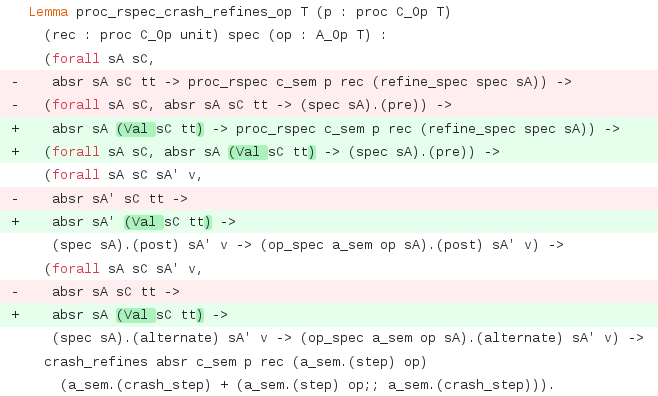
\includegraphics[width=1.0\textwidth]{maintenance/fig/patch.png}
  \caption{Patches to a lemma by an expert proof engineer.}
  \label{fig:patch}
\end{figure}

Changes to programs and specifications were often formulaic and repetitive.
For example, Figure~\ref{fig:patch} shows an example change by an expert proof engineer.
In this change, the proof engineer wraps two arguments into a single application of \lstinline{Val}
in three different hypotheses of a lemma.
This change did not occur in isolation: the proof engineer patched 10 other definitions or lemmas
in similarly, wrapping arguments into an application of
\lstinline{Val}.
%I suspect that this was due to a change in the definition of \lstinline{absr},
%but I was not able to confirm this since
%the change in question occurred before the beginning of the study.

Changes to programs and specifications did break proofs, even for expert proof engineers.
The proof engineers most often (75\% of the time) fixed broken proofs by stepping 
up above those proofs in the UI and fixing something else, like a specification.
That is, development and maintenance were in reality tightly coupled.

But sometimes, proof engineers did not successfully fix proofs broken by changes in programs and specifications.
For example, for the change in Figure~\ref{fig:patch},
the expert proof engineer admitted or aborted (that is, gave up on) the proofs of four of the five
broken lemmas after this change.
In other words, right now, even experts sometimes just give up in the face of change.

TODO: And it's an extra big problem when you have a large development and the changes are outside of your control.

TODO: Hence Social Processes.

TODO: Why automation breaks, even with good development processes.
In other words, even experts are human.
And automation doesn't understand how things change, so can't help the human out.
But proof repair---smarter proof automation---can.

% TODO for now, just a copy-paste of analytics original paper, including the bib---will change soon

%\section{Introduction}

%Proof assistants allow programmers to verify everything from distributed systems~\cite{wilcox:verdi} and compilers~\cite{leroy:compcert} to
%formalizations of mathematics~\cite{DBLP:journals/corr/BauerGLSSS16}. 

Proof automation makes verification more accessible to programmers, but it is often intractable
without programmer guidance. In \textit{interactive theorem proving} (ITP), the programmer guides the 
proof search process. The guidance reduces the search space to make proof automation more tractable.
This in turns helps the programmer, who does not have to manually verify the entire system.

%Interactive theorem provers allow programmers to guide proof search and interactively 
%verify everything from distributed systems~\cite{wilcox:verdi} and compilers~\cite{leroy:compcert} to
%formalizations of mathematics~\cite{DBLP:journals/corr/BauerGLSSS16}. In many of these theorem provers, programmers use

%In these languages, programmers write precise specifications of programs
%and prove implementations correct with respect to the specifications.

Despite automation, programming in these proof assistants is brittle: Even a minor change to a definition or theorem
can break many dependent proofs. This is a major source of development inefficiency in proof assistants
based on dependent type theory~\cite{proof-eng, Aydemir2008, Delaware2013ICFP}.

Traditional proof automation does not consider how proofs, definitions, and theorems change over time.
Instead, it is driven by the state of the current proof, sometimes with supplementary
information from other proofs, definitions, and theorems (as in hint databases~\cite{hints} and rippling~\cite{rippling}).
This puts the burden of dealing with brittleness on the programmer. 

We present a new approach to proof automation that accounts for breaking changes. %:
%searching the difference in versions of a proof, definition, or theorem. 
%We reimagine the problem of proof reuse~\cite{Boite2004, Mulhern06proofweaving} 
%in the context of traditional automation for ITP. 
In our approach, the programmer guides proof search 
by providing an \textit{example} of how to adapt proofs to changes in definitions or theorems.
A tool then generalizes the example adaptation into a \textit{reusable patch} that the programmer can use to fix
other broken proofs.

In doing so, we chart a path for a future %of ITP 
that moves the burden of brittleness
away from the programmer and into proof automation. 
Programmers typically address brittleness through design principles that make proofs
resilient to change~\cite{proof-eng, Aydemir2008, Delaware2013ICFP}, or through program-specific proof automation~\cite{chlipala:cpdt}.
These techniques, while useful, have limitations: 
Planning a verification effort around future change is challenging, and program-specific automation requires specialized knowledge.
The programmer's ability to anticipate likely changes determines the robustness of both techniques in
the face of change. %The robustness of both techniques in the face of change is determined by the programmer's ability to anticipate likely changes. 
Even then, many breaking changes are outside of the programmer's control. Updating proof assistant
versions, for example, can break proofs regardless of planning or automation~\cite{verdicommit}.

\begin{figure*}[ht]
\begin{minipage}{0.48\textwidth}
\centering
\lstset{language=coq, aboveskip=0pt, belowskip=0pt}
\lstinputlisting[firstline=1, lastline=3]{repair/izr.tex}
\lstinputlisting[backgroundcolor=\color{orange!35},firstline=4,lastline=5]{repair/izr.tex}
\lstinputlisting[firstline=6, lastline=6]{repair/izr.tex}
\end{minipage}
\hfill
\begin{minipage}{0.48\textwidth}
\centering
\lstset{language=coq, aboveskip=0pt, belowskip=0pt}
\lstinputlisting[firstline=8, lastline=10]{repair/izr.tex}
\lstinputlisting[backgroundcolor=\color{orange!35},firstline=11,lastline=12]{repair/izr.tex}
\lstinputlisting[firstline=13, lastline=13]{repair/izr.tex}
\end{minipage}
\vspace{-.3cm}
%\setlength{\belowcaptionskip}{-2pt}
\caption[Caption]{Old (left) and new (right) definitions of \lstinline{IZR} in Coq.
The old definition applies injection from naturals to reals and conversion of positives to
naturals; the new definition applies injection from positives to reals.}
\label{fig:izr}
\end{figure*}


We identify a set of core components that are critical to searching an example for patches in Coq.
We use the components to build %four different 
a procedure for finding patches %for non-structural changes 
in a Coq plugin as a 
proof-of-concept.
Case studies on real projects like CompCert~\cite{leroy:compcert} and the Coq standard library
suggest that patches are useful for realistic scenarios, and that it is simple to compose the components 
to handle different classes of changes.
We test the boundaries of the components on a suite of tests
and show how our findings can help build the future we envision.

In summary, we contribute the following:

\begin{enumerate}
%\item We develop new foundations for proof automation in ITP that account for breaking changes. % TODO reword
\item We identify a set of core components that are key to searching for patches.
\item We demonstrate that these core components are useful on real changes in Coq code.
\item We explore how to drive a future that moves the burden of change in ITP away from the programmer and into automated tooling.
\end{enumerate}

% TODO fix contributions

% evaluation stuff in contributions too

% SOMEWHERE: we focus on non-structural changes





%\section{Building \toolname}
\label{sec:plugin}

\toolname is a tool that collects fine-grained proof development data.
%without relying on a particular UI.
It is available on Github for Coq 8.10, with backported branches for
Coq 8.8 and Coq 8.9.\footnote{\url{http://github.com/uwplse/coq-change-analytics}}

\toolname works by instrumenting Coq to listen to user interaction.
Coq's interaction model (Section~\ref{sec:repl}) implements a REPL,
or Read Eval Print Loop: a loop that continually reads in messages
from the user, evaluates the statements those messages contain, 
and prints responses to the user.
All UIs for Coq, from the command line tool
\lstinline{coqtop}~\cite{coq-commands} to the IDEs CoqIDE~\cite{coqide} and
Proof General~\cite{Aspinall2000}, communicate with Coq through the REPL.
\toolname instruments the REPL to collect fine-grained data while remaining
decoupled from the UI.

Figure~\ref{fig:design} summarizes the design of \toolname.
\toolname is made of two parts: a client that the user installs,
and a web server that stores the data from multiple users.
The client instruments the REPL to record and log the data that the
user's UI sends to Coq (Section~\ref{sec:client}),
then sends this data to the server (Section~\ref{sec:server}),
which stores it for analysis.

The implementation effort for \toolname was modest, with just 412 LOC
of OCaml for the client and 178 LOC of Python for the server.%
\footnote{Counted using David M. Wheeler's SLOCCount.}
This modest effort was enough for us to collect 
(Section~\ref{sec:deployment}) and analyze 
(Sections~\ref{sec:q1} and~\ref{sec:q2}) data from hundreds
of interactive sessions.

\subsection{User-Coq Interaction}
\label{sec:repl}

% Is there a better source than this: http://paral-itp.lri.fr/papers/files/coq-workshop-paper.pdf
The \toolname client listens for messages that the user's UI
sends to Coq's REPL.
To provide a common API for different UIs, the implementation of
Coq's REPL is organized into an interactive state machine.
Each state can include tactics in Coq's tactic language Ltac or commands
in Coq's vernacular; both of these can reference terms in Coq's
specification language Gallina.
When a UI sends a message to Coq's REPL, the message contains a state
machine statement (a labeled transition) that instructs Coq to do one of three things:

\begin{enumerate}
\item \textit{Add}: produce a new state
\item \textit{Exec}: execute an existing state to receive a response
\item \textit{Cancel}: back up to an existing state
\end{enumerate}
Coq reacts accordingly, then returns an ID for the new state
that corresponds to the statement.

Taken together, these three statement types can be used
to reconstruct the proof engineer's behavior,
such as defining and redefining types, interactively constructing proofs,
and stepping up when the user hits a dead-end.

% Talia: Trying to get latex to display this in a reasonable place
\begin{figure}
  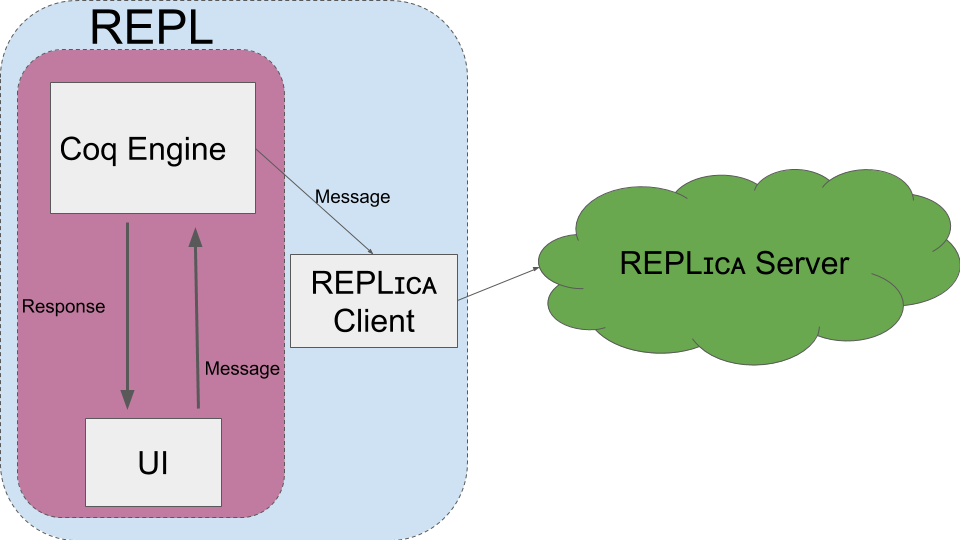
\includegraphics[width=0.8\columnwidth]{maintenance/fig/architecture.png}
\caption{\toolname design. The \toolname client listens to the REPL
and sends data to the \toolname server.}
\label{fig:design}
\end{figure}

\paragraph{From User Behavior to the State Machine}
When the user runs a command or tactic in Coq, the UI first adds
a new state corresponding to the command or tactic.
Adding a state to the state machine does not actually execute the
command or tactic;
to do that, the UI must execute the new state.
In other words, in state machine terms, each addition follows a transition,
but only returns the state number.
To get the state information, the UI must call \textit{Exec}.

Using this mechanism, the UI can group state machine statements and execute them
all at once. %, without interacting with the intermediate states.
For example, stepping down past 3 definitions at once in an IDE
manifests as 3 additions followed by a constant
number of executions, and successfully compiling a file manifests as 
many additions followed by a constant number of 
executions.\footnote{Some UIs send Coq multiple executions for each
group of additions.} 

When the user steps up in the UI, or attempts to run a tactic or command
that fails, the UI backs up to an existing state in the state machine.
Sending the state machine a cancellation statement is not the only way to back up to
an existing state; cancellations can also take the form of state machine
\textit{additions} of \lstinline{Cancel} or \lstinline{BackTo} commands
in Coq's vernacular. In either form, cancellations take a state ID
as an argument to specify the state to back up to.
%% Trying a statement that fails manifests as a cancellation,
%% and stepping up in an IDE manifests as a cancellation
%% followed by an IDE signature;
%% Section~\ref{sec:discussion} discusses distinguishing between these.

\paragraph{An Example: Defining and Extending an Inductive Type}
To see how user behavior corresponds to state machine statements,
consider an example from User 1, Session 41, simplified for readability.
In this session, User 1 stepped past
the definition of an inductive type \lstinline{Alpha}. Later, User 1
stepped above \lstinline{Alpha}, imported list notations,
then stepped down to add a new constructor to \lstinline{Alpha}
using those notations.

When User 1 first stepped down below \lstinline{Alpha},
Coq received a state machine addition (denoted
\lstinline{Add}, following SerAPI~\cite{GallegoArias2016SerAPI})
of this definition (again simplified for readability):

\begin{lstlisting}
  (Add () "Inductive Alpha : $\ldots$ := $\ldots$")
\end{lstlisting}
at the state ID \lstinline{1}, producing state ID \lstinline{2}.
Since User 1 stepped down a single step, Coq also received
an execution (denoted \lstinline{Exec}) of the new state:

\begin{lstlisting}
  (Exec 2)
\end{lstlisting}
which did not produce a state with a new state ID, since only additions
produce states, and only states have state IDs.
When User 1 stepped up to above the definition of \lstinline{Alpha},
Coq received a cancellation (denoted \lstinline{Cancel}):

\begin{lstlisting}
  (Cancel 1)
\end{lstlisting}
taking the state machine to before the definition of \lstinline{Alpha}.
When User 1 added the import, Coq
received an addition at state ID \lstinline{1}, producing state ID
\lstinline{3}, followed by an execution:

\begin{lstlisting}
  (Add () "Import Coq.Lists.List.ListNotations. ")
  (Exec 3)
\end{lstlisting}
Finally, when User 1 added the new constructor to \lstinline{Alpha}
and stepped down past it,
Coq received an addition of \lstinline{Alpha} with the new
constructor at state ID  \lstinline{3} producing state ID \lstinline{4}, followed by an execution:

\begin{lstlisting}
  (Add () "Inductive Alpha : $\ldots$ := $\ldots$
             | alpha_rec_mt : $\ldots$")
  (Exec 4)
\end{lstlisting}

The data that \toolname received provided us with enough
information to visualize these changes as a sequence of
diffs for later analysis (Section~\ref{sec:q2}).
As a consequence, we were able to find this pattern of development
of incrementally extending inductive types for four of our users
(Section~\ref{sec:pat1}).

\subsection{User-Client Interaction}
\label{sec:client}

The \toolname client records all of the additions, executions,
and cancellations that the proof engineer's UI or compiler sends.
To use it, the proof engineer installs the client,
then adds a line to the Coq requirements file~\cite{coqrc} so that
Coq always loads it.
On the first build, \toolname asks the proof engineer for consent and
for demographic information for the study.
From then on, the proof engineer uses Coq normally.

The implementation of the client is a Coq plugin.
Coq's plugin system makes it possible to extend
Coq without compromising trust in the Coq core.
\toolname does not include new commands or tactics; it simply attaches
to Coq's REPL and listens for messages that the proof engineer sends to Coq.

The hooks in the plugin API that allow plugins to listen to the REPL
were not initially present in Coq;
we worked with one of the Coq developers
to add this to Coq 8.10.\footnote{\url{http://github.com/coq/coq/pull/8768}}
We also developed backported branches of Coq 8.8 and 8.9 that include
this API, so that users whose projects depended on those
versions of Coq could participate in our study. This API is now available in all
versions of Coq going forward. %so that other study and plugin authors
%can use it.

\subsection{Client-Server Interaction}
\label{sec:server}

To record a history of user behavior,
the \toolname client sends a record of each state machine addition,
execution, and cancellation to the \toolname server.
The server then collects this data into a format suitable for analysis.

The message that the client sends to the server includes both the
state machine statement and additional metadata.
\iffalse
For example, a full message to the server for the simplified example
from Section~\ref{sec:repl} looks like this:

\begin{lstlisting}
((time 1567665712.25)
 (id 2)
 (user 1)
 (session-module gamma_completeness_implies_ec_assoc)
 (session 1567665710.63)
 (Control
   (Add () "Inductive Alpha : $\ldots$ := $\ldots$")))
\end{lstlisting}
where \lstinline{time} is the time the state change occurred,
\lstinline{id} is the state of the addition,
\lstinline{user} is the user ID,
\lstinline{session-module} is the Coq module in which the statements
were executed,
\lstinline{session} is the start time of the session,
and the body of the messages beginning with \lstinline{Control}
is the addition to the state machine.
%\todo{what do we do about our off-by-one errors?}
\fi

\begin{figure*} % Talia: For good table placement
\begin{minipage}{0.67\textwidth}
\small
\centering
\begin{tabular}{ |l|l|l|l|l|l|l| }
 \hline
  \textbf{User} & \textbf{Years} & \textbf{Expertise} & \textbf{Purpose} & \textbf{Frequency} & \textbf{UI} & \textbf{Version} \\
\hline
  \textbf{0} & 2-4 & $\circ$ $\circ$ $\circ$ $\circ$ $\circ$ & Verification & Daily & Proof General & Master \\
  \textbf{1} & 2-4 & $\circ$ $\circ$ $\circ$ & Mathematics & Monthly & Proof General & 8.10 \\
  \textbf{2} & > 4 & $\circ$ $\circ$ $\circ$ $\circ$ & Verification & Daily & Proof General & 8.10 \\
  \textbf{3} & > 4 & $\circ$ $\circ$ $\circ$ $\circ$ $\circ$ & Verification & Weekly & Proof General & Master \\
  \textbf{4} & > 4 & $\circ$ $\circ$ $\circ$ $\circ$ & Verification & Daily & coqtop & Master \\
  \textbf{5} & 2-4 & $\circ$ $\circ$ $\circ$ & Verification & Monthly & Custom & 8.10 \\
  \textbf{6} & 2-4 & $\circ$ $\circ$ $\circ$ $\circ$ & Mathematics & Daily & Proof General & Master \\
  \textbf{7} & 2-4 & $\circ$ $\circ$ $\circ$ $\circ$ & Mathematics & Weekly & Proof General & 8.10 \\
  \textbf{8} & > 4 & $\circ$ $\circ$ $\circ$ $\circ$ $\circ$ & Verification & Daily & Proof General & 8.8 \\
  \textbf{9} & > 4 & $\circ$ $\circ$ $\circ$ $\circ$ $\circ$ & Verification & Monthly & Proof General & 8.9 \\
  \textbf{10} & > 4 & $\circ$ $\circ$ $\circ$ & Verification & Daily & Proof General & 8.8 \\
  \textbf{11} & > 4 & $\circ$ $\circ$ $\circ$ & Mathematics & Daily & Proof General & 8.9 \\
\hline
\end{tabular}
\caption{User profiles of Coq development
background: experience in years, self-assessed expertise (beginner, novice, intermediate, knowledgeable, or expert, represented by circles), purpose of use, frequency of use, UI, and current version.}
\label{tab:users}
\end{minipage}
\hfill
\begin{minipage}{0.31\textwidth}
\small
\centering
\begin{tabular}{ |l|l|l|l| }
 \hline
  \textbf{User} & \textbf{Total} & \textbf{Interactive} & \textbf{Proof}\\
\hline
  \textbf{0} & 6 &  0 & 0 \\
  \textbf{1} & 42 & 10 & 4 \\
  \textbf{2} & 7 & 3 & 0 \\
  \textbf{3} & 11495 & 101 & 8 \\
  \textbf{4} & 1 & 0 & 0 \\
  \textbf{5} & 41 & 15 & 16 \\
  \textbf{6} & 1 & 0 & 0 \\
  \textbf{7} & 229 & 183 & 241 \\
  \textbf{8} & 162 & 27 & 10 \\
  \textbf{9} & 5 & 0 & 0 \\
  \textbf{10} & 23 & 15 & 0 \\
  \textbf{11} & 17 & 8 & 0 \\
\hline
\end{tabular}
\caption{Number of total sessions, interactive sessions,
  and interactive proof subsessions per user.}
\label{tab:sessions}
\end{minipage}
\end{figure*}

\paragraph{Metadata for Two Challenges}
The metadata beyond the state ID and the state machine
statement exists to handle two challenges:
The first challenge is that state machine interactions alone
are not enough to reconstruct a per-user history,
nor to group the user's interaction into discrete sessions
for a particular project or module.
The second challenge is that the network can be slow or unreliable at times,
causing messages to be received by the server out of order,
and slowing down the UI if not handled properly.

To handle the first challenge, \toolname labels each message with
a module name, user ID, and session ID.
The module name comes from the Coq plugin API.
The user ID is generated by the server and stored on the user's machine.
\iffalse
When a user builds the client for the first time, it contacts the server
and receives a unique user ID, which is stored locally on the
user's machine.
\fi
The session ID, in contrast, is generated by the client:
When the user loads the client, upon opening any new file,
the client records the start time of the session.
This start time is then used to identify the session.

To handle the second challenge, \toolname{} labels each message
with two pieces of metadata: the time at which the state machine message was sent to Coq (to order messages)
and the state ID (to detect missing states).
TCP alone is not enough to address these issues since each invocation
of the plugin creates a separate network stream
(so the server may receive messages out of order),
and since the user can disable the plugin
(so the client may never send some 
messages).\footnote{The consent form allowed users to temporarily disable
the plugin if necessary, as long as they informed us of this.} 
In addition to this metadata,
%instead of sending messages as soon as they are ready,
\toolname{} sends messages in batches.
If the network is not available, \toolname{} logs messages locally,
then sends those logs to the server the next time
the network is available.


%\section{Deploying \toolname}
\label{sec:deployment}

We set out to answer the following questions:

\begin{itemize}
\item \textbf{Q1}: What kinds of mistakes do users make in interactive proofs, and how do they fix them? (Section~\ref{sec:q1})
\item \textbf{Q2}: What kinds of changes to programs and specifications do users
make often, and do those changes reveal patterns amenable to automation? (Section~\ref{sec:q2})
\end{itemize}
To answer these questions, we recruited 12 proof
engineers to install \toolname and use Coq normally for
a month (Section~\ref{sec:recruiting}).
We received a month's worth of data containing granular detail on
Coq development for 8 of 12 of those users
(Section~\ref{sec:collection}).
After a month, we shut down the server, closed the study,
and visualized and analyzed the data (Section~\ref{sec:analysis}).

\subsection{Recruiting}
\label{sec:recruiting}

We recruited proof engineers by distributing a promotional video
and study description.
\iffalse
 to the \lstinline{coq-club} email list, on Twitter,
and directly to professors at universities with many Coq users.
\fi
All potential users went through a screening process, ensuring that they are
at least 18 years old, fluent in English, and have at least a year of experience using Coq.
Upon installation of the plugin, users filled out a consent form.
Users then filled out a questionnaire about Coq background and usage,
the results of which are in Figure~\ref{tab:users}.

All users reported more than 2 years of experience;
7 reported more than 4.
Self-assessed expertise was evenly distributed between intermediate,
knowledgeable, and expert; no beginners or novices participated.
4 users reported that they use Coq for writing mathematical proofs,
while the other 8 reported that they use Coq for verifying software.
7 users said that they use Coq every day, 2 a few times per week,
and 3 a few times per month.
10 users reported using Proof General, while 1 user reported using
\lstinline{coqtop}, and 1 user reported using a custom UI.
4 users installed the plugin with the master branch of Coq,
while 4 users used Coq 8.10, 2 users used Coq 8.9,
and 2 users used Coq 8.8.

\subsection{Collection}
\label{sec:collection}

The study period lasted one month, during which users agreed to develop
Coq code with the plugin enabled whenever possible, or otherwise let us know
why this was not possible.
All of the data collected within this time period
has been made publicly available with the consent of the users.\footnote{\url{http://github.com/uwplse/analytics-data}}

Figure~\ref{tab:sessions} shows the number of sessions by user.
Every time the plugin was loaded, either inside of a compiled file
or inside of a file open in a UI, this began a new session.
For both Q1 and Q2, our analyses looked for changes only within
sessions that involved some combination of failure
and stepping up and then back down in a UI;
we call these \textit{interactive sessions}.

We marked a session as interactive if it contained at least
one cancellation followed by other changes in
state. This did not capture any compilation passes
because Coq disallows cancellations outside of interactive mode.
For example, User 3 logged 11495 total sessions, only 101
of which were interactive. 
The remainder of User 3's sessions were, for the most part,
compilation passes over large sets of dependencies (one session per dependency).
In total, across all users, there were 362 interactive sessions.

Within these interactive sessions, the analysis for Q1 looked for 
fixes to failing tactics only inside of spans of time spent 
\emph{inside proofs} that involved some combination of failure and
stepping up and then back down in a UI;
we call these \textit{interactive proof subsessions}.
There could be zero, one, or multiple of these within an interactive session.
We detected these similarly to how we detected
interactive sessions.
There were 279 interactive proof subsessions.

\toolname logged interactive sessions for only 8 of the 12 users.
Section~\ref{sec:discussion} discusses possible causes of, implications of,
and remedies for this.
%We speculate as to why, consider the implications,
%and discuss how to reach more users in Section~\ref{sec:discussion}.

\subsection{Analysis}
\label{sec:analysis}

Once we had collected this data, we analyzed it to answer Q1 and Q2.
To answer these questions, we developed a small Python
codebase to analyze the data.
The scripts used information about cancellations
to build visualizations to aid in analysis.
For Q1, we built this cancellation information into a search tree for
each proof, and produced visualizations of each tree
(see \Cref{fig:search-tree}).
For Q2, we used this cancellation
information to reconstruct a sequence of diffs, and used Git tooling
to manually inspect these diffs (see \Cref{fig:ex-diff}).

The scripts, visualizations, and results for Q1 and Q2 can
be found alongside the data in the public data repository. 

\section{Q1: Mistakes In and Fixes to Proofs}
\label{sec:q1}

Q1 asked what mistakes proof engineers
make in proofs, and how they fix those mistakes.
This data may inform the development of tools
that help users write proofs
by suggesting next steps and changes to existing tactics.

\paragraph{A1}
We found the following:

\begin{enumerate}
\item Most interactive proof subsessions ended
  in the user stepping up to an earlier definition.
This shows that writing definitions and proofs about those definitions was
usually a feedback loop. (Section~\ref{sec:feedback})
\item Within proofs, application of lemmas
was the main driver of proving. (Section~\ref{sec:tactics})
\item Within proofs, over half of fixes to tactic mistakes
fixed either an improper argument or wrong sequencing structure.
(Section~\ref{sec:fixes})
\end{enumerate}

\paragraph{Methodology}
Our analysis for Q1 looked within the 279 interactive proof subsessions.
We first counted the number of times each tactic was used, the number
of times it was stepped above, and the number of times its invocation
caused an error. Then, we constructed a search tree using the
cancellation structure, and for any state which had multiple out edges
(a proof state where multiple tactics were tried), we compared the
cancelled attempts to the final tactic used.

\subsection{Fixing Proofs by Fixing Definitions}
\label{sec:feedback}

Of the 279 interactive proof subsessions, 209 (over 75\%) began a proof,
only to step above the entire proof attempt and
return to make changes to earlier definitions or commands, for example
to change a specification to make the proof possible.
This suggests that tools that attempt to provide next steps to users writing proof
may also benefit from suggesting possible fixes to definitions used in the proof.
% ,as the proof often cannot be completed without first changing definitions.
% ^ Talia: We can't claim "often cannot," but I think it's OK to omit
\begin{displayquote}
  \textbf{Takeaway:}
  It may be beneficial to combine machine learning tools
  that automatically complete or suggest hints for
  proofs~\cite{proverbot9001, Komendantskaya2012, Nagashima2018, Gauthier2017b,
    Yang2019}
  with tools for repairing definitions~\cite{Ringer2018, robert2018}.
\end{displayquote}

We considered only the remaining 70 successful interactive proof subsessions
(made up of 1085 tactic invocations)
for the sake of analyzing behavior \textit{within} proofs that
ended in a successful proof.
The analysis for Q2 (Section~\ref{sec:q2}) reveals more about
how specifications and programs changed.

\begin{figure}
\small
  \begin{tabular}{|l|c|c|c|}
    \hline
    \textbf{Tactic} & \textbf{Used} & \textbf{Failed} & \textbf{Stepped Above} \\
    \hline
    apply& 156& 27& 13\\
    intros& 108& 16& 5\\
    destruct& 94& 24& 12\\
    rewrite& 61& 13& 12\\
    exists& 47& 9& 1\\
    unfold& 45& 2& 8\\
    simpl& 32& 6& 4\\
    reflexivity& 27& 1& 1\\
    simpl in& 25& 3& 7\\
    assumption& 24& 2& 1\\
    specialize& 19& 0& 1\\
    subst& 14& 1& 0\\
    split& 12& 0& 0\\
    eapply& 11& 0& 5\\
    dependent& 10& 0& 8\\
    inversion& 10& 0& 0\\
    constructor& 10& 3& 0\\
    eauto& 9& 0& 4\\
    assert& 9& 2& 0\\
    induction& 8& 0& 1\\
    validate& 8& 0& 5\\
    monoid& 7& 0& 2\\
    tauto& 7& 1& 0\\
    eassumption& 7& 0& 5\\
    repeat constructor& 7& 0& 5\\
    \hline
  \end{tabular}
  \caption{The top 25 most common tactics.}
\label{fig:tactics-table}
\end{figure}

\subsection{Tactics Used and Cancelled}
\label{sec:tactics}

\begin{figure*}
  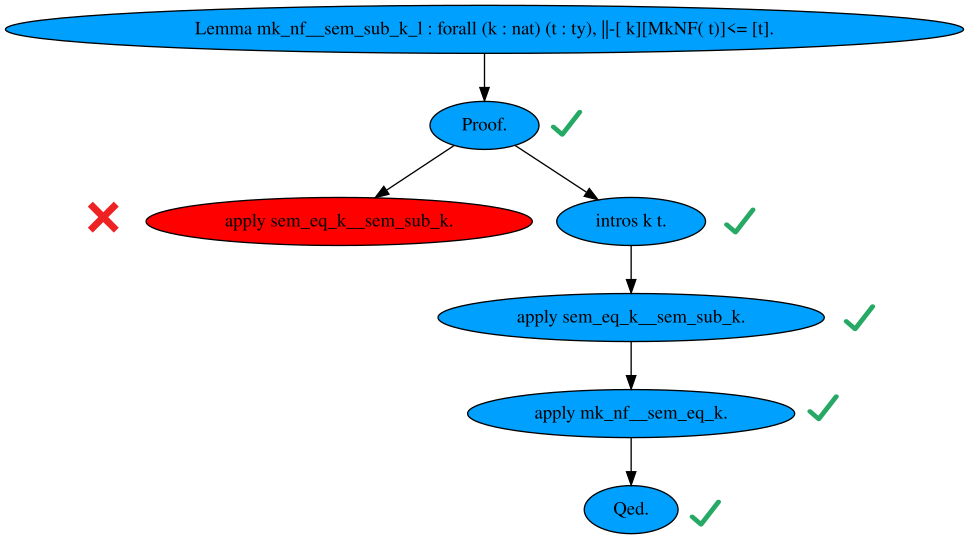
\includegraphics[width=0.70\textwidth]{maintenance/fig/example-graph.png}
  \caption{An example search tree, generated from the collected data
    by \toolname. It shows the user attempting to apply a lemma, which
    fails until they first run the \lstinline{intros} tactic.}
  \label{fig:search-tree}
\end{figure*}

\Cref{fig:tactics-table} shows the counts for each tactic
(regardless of arguments) in the 70 successful interactive proof subsessions.
%From this table, we can see that the
The distribution of tactics run was top-heavy; over 50\% of the tactics
invoked were either \lstinline{apply}, \lstinline{intros},
\lstinline{destruct}, \lstinline{rewrite}, \lstinline{exists}, \
\lstinline{unfold}, or \lstinline{simpl}.
The \lstinline{apply} tactic had a significant lead over other tactics
in invocations, but invocations of \lstinline{destruct} ended in
failure or stepping above them nearly as many times as invocations
of \lstinline{apply} did.

This data indicates two takeaways for proof tooling:
Firstly,
\begin{displayquote}
  \textbf{Takeaway:}
  Tools may be able to focus on understanding the behavior of
  and suggesting just a small number of tactics,
  and still benefit.
\end{displayquote}
And second, since lemma and hypothesis application was the main driver of proofs,
\begin{displayquote}
  \textbf{Takeaway:}
  Assessing which lemmas and hypotheses are useful would be one of the main tasks of
  a tool which suggests tactics to the user.
\end{displayquote}
The machine learning tool ML4PG~\cite{Komendantskaya2012} for Coq
already offers promising developments in this direction by understanding
and providing hints about similar lemmas,
as does the proof automation tool CoqHammer~\cite{coqhammer};
similar functionality may help
improve the performance of tools that suggest tactics.

\subsection{Fixing Proofs by Fixing Tactics}
\label{sec:fixes}

%While the raw cancellation numbers are useful, they do not give a
The raw cancellation numbers do not give a
broader context to each cancellation, namely what tactic it was
cancelled in favor of. To address this, we built a search
graph and analyzed the tactic attempts at each branching node (see
\Cref{fig:search-tree}). Where there were more than 2 attempts, we
compared all non-final attempts to the final one separately.

In our 71 successful interactive proof subsessions, 96 tactics
were cancelled in favor of another tactic at the same state.
Of the 96 cancelled-tactic and final-tactic pairs: %, we found:
\begin{itemize}
\item 13 were semicolon clauses added after a tactic, like:
  \begin{lstlisting}
    destruct w. $\to$ destruct w; reflexivity.
  \end{lstlisting}
\item 4 were semicolon clauses removed from the end of a tactic, like:
  \begin{lstlisting}
    intros; reflexivity. $\to$ intros.
  \end{lstlisting}
\item 31 were the same tactic with modified arguments, like:
  \begin{lstlisting}
    intros k X t. $\to$ intros k X t Hfresh.
  \end{lstlisting}
\item 5 were similar, but a \lstinline{Search} or \lstinline{Check} command was first run
  before replacing the tactic, like:
  \begin{lstlisting}
    apply IdSetFacts.remove_3. $\to$ 
    Check IdSetFacts.remove_3. 
    apply IdSetFacts.remove_3 with Y.
  \end{lstlisting}
\item 43 changes did not fall into this categorization.
\end{itemize}

The proofs shown were complex, and users often made nontrivial
changes to attempted tactics, so not all changes could be
easily categorized or analyzed. However, over half of the changes
present could be categorized into simple changes, and potentially
synthesized by automated tools.

This data also shows us that for a large proportion of tactics, users
could correctly pick the tactic to invoke, even when they made
mistakes in its arguments. In addition, fixing these arguments took both
on average and in the worst case longer than fixing other kinds
of mistakes. Accordingly,
\begin{displayquote}
  \textbf{Takeaway:}
  Automated tooling that suggests actions to take
  based on tactics that were recently stepped above or failed
  may focus on predicting new arguments for the attempted tactic.
\end{displayquote}

\section{Q2: Changes to Terms}
\label{sec:q2}

Q2 asked what kinds of changes proof
engineers make to programs and specifications, and whether those
changes reveal patterns amenable to automation.
This information may be useful to ensure tools for proof evolution
support the features that help proof engineers.

\paragraph{A2}
We found that while no single change was dominant across
all users, users made related changes within and across sessions.
Analysis of these changes revealed four patterns:

\begin{enumerate}
\item Incremental development of inductive types
\item Repetitive refactoring of identifiers
\item Repetitive repair of specifications
\item Interactive discovery of programs and specifications
\end{enumerate}

\paragraph{Methodology}
To answer this question, we wrote a script to visualize changes over 
time as diffs on Github (see Figure~\ref{fig:ex-diff}).
The script reconstructed the state of the file up to 
each cancellation within a session, then committed that to the 
public data repository.
When possible (see Section~\ref{sec:wish2}), it augmented
each commit with information on whether the cancellation was a failure
or the user stepping up in an IDE.

We then manually analyzed the diffs that this visualization produced to 
build a classification of changes (Section~\ref{sec:class}), 
then classify changes that we found (Section~\ref{sec:changes}).
We did this for each of the 362 interactive sessions and, when relevant,
across sessions as well.
Finally, we looked at clusters of common changes for patterns.
For each of the four patterns we found
(Sections~\ref{sec:pat1},~\ref{sec:pat2},~\ref{sec:pat3}, and~\ref{sec:pat4}),
we identified benchmarks (examples of the pattern in our data)
and lessons for automation.

\subsection{Building a Classification}
\label{sec:class}

After running the visualization script, we did a manual analysis of the diffs
in order to build a classification of changes to Gallina terms.
This analysis was thorough in that it involved inspecting each
consecutive diff and, when relevant, diffs that spanned several commits
(when a user stepped up, changed something, and then later stepped back down)
or sessions (when a user modified the same file during two different sessions).
However, it did not necessarily capture all changes to terms;
Section~\ref{sec:wish2} discusses some of the challenges.

\paragraph{Classification}

We designed a classification that groups changes along three dimensions:

\begin{enumerate}
\item \textbf{Command}: vernacular command used to define the term in
                        which a subterm changed
\item \textbf{Operation}: how the subterm changed
\item \textbf{Location}: innermost subterm that changed
\end{enumerate}
with the following categories for \textbf{Operation}:

\begin{enumerate}
\item \textbf{Structure}:
\begin{enumerate}
\item \textbf{Add} or \textbf{Del}: add or delete information
\item \textbf{Mov}: move information
\end{enumerate}
\item \textbf{Content}:
\begin{enumerate}
\item \textbf{Pch} or \textbf{Uch}: patch or unpatch
\item \textbf{Cut} or \textbf{Uut}: cut or uncut
\item \textbf{Rpl}: replace
\end{enumerate}
\item \textbf{Syntax}:
\begin{enumerate}
\item \textbf{Rnm}: rename
\item \textbf{Qfy} or \textbf{Ufy}: qualify or unqualify
\end{enumerate}
\end{enumerate}
Changes listed together are inverse operations.
The \textbf{Structure} changes are straightforward.
Among the changes to \textbf{Content}, \textbf{Pch} is applying a function
to the old term to get a new term, \textbf{Cut} is defining a new term
or let-binding and then referring to that term inside of an existing term,
and \textbf{Rpl} is replacing contents in any other way.
Among the \textbf{Syntax} changes, \textbf{Qfy} is
qualifying a constant after changing an import.

For \textbf{Structure} changes, there are five \textbf{Location}s:

\begin{enumerate}
\item \textbf{Hyp}: hypothesis of anything that can take arguments
\item \textbf{Arg}: argument in an application
\item \textbf{Ctr}: constructor of an inductive type
\item \textbf{Cas}: case of a match statement
\item \textbf{Bod}: body of anything that can take arguments
\end{enumerate}

For \textbf{Content} changes, there are an additional two:

\begin{enumerate}
\setcounter{enumi}{5}
\item \textbf{Fun}: function in an application
\item \textbf{Typ}: type annotation
\end{enumerate}

For \textbf{Syntax} changes, there are only three:

\begin{enumerate}
\item \textbf{Bnd}: binding in the local environment
\item \textbf{Idn}: identifier in the global environment
\item \textbf{Con}: constant
\end{enumerate}

\paragraph{Design Considerations}

That classification that we designed considers changes only within
Gallina terms defined or stated using vernacular commands.
Since it is focused solely on changes to defined terms,
it does not consider other information like changes to vernacular commands,
hints, tactics, notations, scope annotations, inference information, or imports,
and it considers additions of new terms only in \textbf{Cut} changes.

In building this classification, we aimed to group
changes at a level of granularity narrow enough to inform the design of proof
engineering tools, but broad enough to capture patterns.
We suspect that within these categories, there are more granular
categories that can be useful for automation, like distinguishing among
hypotheses to set apart indices of inductive types, or classifying
a \textbf{Content} change as semantics-preserving.
We did not design a more granular classification because we did not
find it useful for describing our data.
%(we found no changes to indices of inductive types, for example).

\subsection{Classifying Changes}
\label{sec:changes}

Once we had designed this classification,
we used it to classify the changes that we had found.
We ignored intermediate changes that immediately failed to lex, parse, or type check.

\begin{figure*}
\small
\begin{tabular}{ |l|rrrr|l|l|l| }
\hline
     \textbf{User} &
     \multicolumn{4}{c|}{\textbf{Top Changes}} &
     \textbf{\# Changes} &
     \textbf{\# Interactive} &
     \textbf{Expertise}
\\
\hline
     \textbf{1} &
     \indpat{\textbf{Add} \textbf{Ctr} (23)} &
     \indpat{\textbf{Add} \textbf{Cas} (22)} &
     \refactorpat{\textbf{Qfy} \textbf{Con} \phantom{0}(6)} &
     &
     \phantom{0}69 &
     \phantom{0}10 &
     $\circ$ $\circ$ $\circ$
\\
%\hline
     \textbf{2} &
     \indpat{\textbf{Add} \textbf{Cas} \phantom{0}(4)} &
     &
     &
     &
     \phantom{0}10 &
     \phantom{00}3 &
     $\circ$ $\circ$ $\circ$ $\circ$
\\
%\hline
     \textbf{3} &
     \repairpat{\textbf{Pch} \textbf{Arg} (13)} &
     \pddpat{\textbf{Mov} \textbf{Arg} \phantom{0}(8)} &
     \textbf{Add} \textbf{Bod} \phantom{0}(7) &
     \textbf{Cut} \textbf{Arg} \phantom{0}(7) &
     \phantom{0}55 &
     101 &
     $\circ$ $\circ$ $\circ$ $\circ$ $\circ$
\\
%\hline
     \textbf{5} &
     \indpat{\textbf{Add} \textbf{Cas} (20)} &
     \indpat{\textbf{Add} \textbf{Ctr} (13)} &
     \indpat{\textbf{Add} \textbf{Hyp} (12)} &
     &
     \phantom{0}75 &
     \phantom{0}15 &
     $\circ$ $\circ$ $\circ$
\\
%\hline
     \textbf{7} &
     \refactorpat{\textbf{Rnm} \textbf{Idn} (42)} &
     \pddpat{\textbf{Mov} \textbf{Hyp} (18)} &
     \pddpat{\textbf{Add} \textbf{Hyp} (18)} &
     &
     151 &
     183 &
     $\circ$ $\circ$ $\circ$ $\circ$
\\
%\hline
     \textbf{8} &
     \repairpat{\textbf{Rpl} \textbf{Fun} (29)} &
     \pddpat{\textbf{Del} \textbf{Hyp} \phantom{0}(4)} &
     \pddpat{\textbf{Uch} \textbf{Arg} \phantom{0}(4)} &
     &
     \phantom{0}44 &
     \phantom{0}27 &
     $\circ$ $\circ$ $\circ$ $\circ$ $\circ$
\\
%\hline
     \textbf{10} &
     \pddpat{\textbf{Pch} \textbf{Arg} \phantom{0}(4)} &
     \textbf{Rpl} \textbf{Cas} \phantom{0}(3) &
     &
     &
     \phantom{0}15 &
     \phantom{0}15 &
     $\circ$ $\circ$ $\circ$
\\
%\hline
     \textbf{11} &
     \textbf{Pch} \textbf{Cas} \phantom{0}(3) &
     &
     &
     &
     \phantom{00}7 &
     \phantom{00}8 &
     $\circ$ $\circ$ $\circ$
\\
\hline
\end{tabular}
\caption{Top changes, by user.}
\label{tab:userchanges}
\end{figure*}
% TODO Talia: Check patterns in anything not highlighted
% TODO Talia: Check timestamps and integrate if interesting
% TODO!!! Check user 2 for some constructors.

\begin{figure*}
\begin{minipage}{0.41\textwidth}
\centering
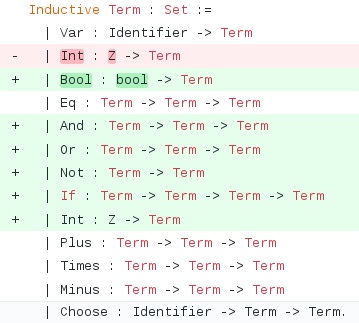
\includegraphics[width=0.7\textwidth]{maintenance/fig/diffs1.png}
\end{minipage}
\hfill
\begin{minipage}{0.57\textwidth}
\centering
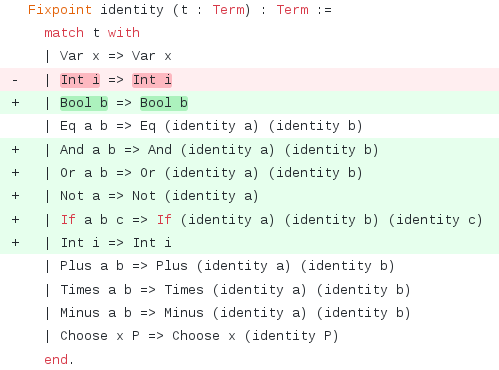
\includegraphics[width=0.7\textwidth]{maintenance/fig/diffs2.png}
\end{minipage}
\caption{A change to an inductive type (left) and corresponding change to a fixpoint (right) that User 5 made in Session 19.}
\label{fig:ex-diff}
\end{figure*}

Classifying changes revealed clusters of related changes.
Further inspection of those clusters revealed common development patterns.
Figure~\ref{tab:userchanges} lists, for each user, the top three changes
by \textbf{Operation} and \textbf{Location} 
(four if there was a tie, and ignoring changes that we found fewer than three times for the user),
the total number of changes that we found,
and the total number of  interactive sessions and self-rated expertise
for reference.
Changes for which more detailed inspection revealed patterns
are highlighted in corresponding colors:
\indpatt{blue} for incremental development,
\refactorpatt{orange} for refactoring, \repairpatt{pink} for
repair, and \pddpatt{grey} for discovery.

The remainder of this section discusses these patterns, complete
with an example, benchmarks, and lessons for automation 
for each.
The benchmarks and lessons for automation are mainly for tool designers:
The benchmarks point to changes in specific sessions, the partial or 
complete automation of which would have helped our users.
The lessons for automation are natural directions for improvements
to proof engineering tools given the patterns we have observed.

The public data repository contains a complete list of the changes
that we classified, as well as a detailed walkthrough of each benchmark.

\subsubsection{Incremental Development of Inductive Types}
\label{sec:pat1}

The most common changes for Users 1 and 5 were adding cases to match statements
(\textbf{Add} \textbf{Cas}) and adding constructors to inductive types
(\textbf{Add} \textbf{Ctr}).
These changes corresponded to incremental development of inductive types,
followed by corresponding extensions to match statements of functions
that destruct over them, or to inductive types that depend
on or relate to them.
This pattern sometimes spanned multiple sessions.
While this pattern was most prevalent for Users 1 and 5, it was also
present for Users 2 and 7.

The diffs in Figure~\ref{fig:ex-diff} show an example change to
an inductive type, along with a corresponding change to a fixpoint.
The change on the left adds five constructors and moves one constructor down.
The change on the right adds five corresponding cases and moves one
corresponding case down.

\paragraph{Benchmark 1}

The example change from \Cref{fig:ex-diff} came from
User 5, Sessions 18, 19, 27, 33, and 35.
There, over the course of three weeks, the user incrementally developed the inductive type \lstinline{Term}
along with a record \lstinline{EpsilonLogic} and fixpoints
\lstinline{simplify} (later renamed to \lstinline{identity}) and \lstinline{free_vars}.

\paragraph{Benchmark 2}

In Sessions 37 and 41, over two days,
User 1 incrementally developed similar inductive types
\lstinline{ST} and \lstinline{GT}, as well as fixpoints
\lstinline{Gamma}, \lstinline{Alpha}, and \lstinline{eq} 
that referred to them.

\paragraph{Lessons for Automation}

Given that several users show this pattern,
this is one use case for which better automation may help.
Automation may help proof engineers adapt other inductive types,
match statements, and proofs after extending inductive types
with new constructors.
We are not aware of any work on adapting related inductive types and 
match statements.
There is some work on adapting proof obligations to new
constructors~\cite{Boite2004},
and a proposed algorithm for generating proofs that satisfy those
obligations~\cite{Mulhern06proofweaving}, but nothing that exists for
a current version of Coq.

\begin{displayquote}
  \textbf{Takeaway}:
  Proof engineers could benefit from automation to help update proofs and definitions
  after adding constructors to inductive types.
  %% Up-to-date automation to help proof engineers adapt definitions
  %% and proofs after extending inductive types is an unaddressed
  %% opportunity make an impact.
\end{displayquote}

\subsubsection{Repetitive Refactoring of Identifiers}
\label{sec:pat2}

Users 1 and 7 showed a pattern of repetitive refactoring, through
qualifying constants after changing imports (\textbf{Qfy} \textbf{Con}),
and renaming identifiers (\textbf{Rnm} \textbf{Idn}) and the constants
that referred to them (\textbf{Rnm} \textbf{Con}), respectively.
This pattern sometimes spanned multiple sessions, and even simple refactorings
sometimes resulted in failures.

Figure~\ref{fig:refactor} shows an example renaming from the five
definitions at the top to the five definitions at the bottom.
The change renames the identifiers of these definitions to
follow the same convention, then makes the corresponding changes
to constants in the bodies of the last two definitions.  

\begin{figure}
  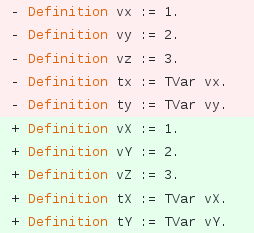
\includegraphics[width=0.19\textwidth]{maintenance/fig/refactor.png}
  \caption{Renaming of definitions in User 7, Session 93.}
  \label{fig:refactor}
\end{figure}

\paragraph{Benchmark 3}

The example from \Cref{fig:refactor} came from User 7, Session 93.
The definition of \lstinline{ty} failed, since User 7 had already
defined an inductive type with that name.
In response, User 7 renamed all of these
to follow the same convention.
This took four attempts, but only a few minutes.

\paragraph{Benchmark 4}

In Session 193, User 7 split the \lstinline{TVar} constructor
of the inductive type \lstinline{ty} into two constructors:
\lstinline{TBVar} and \lstinline{TFVar}. User 7 at the same time
split the fixpoint \lstinline{FV} into \lstinline{FFV} and
\lstinline{FBV}.
In Session 198, User 7 at the same time renamed the broken lemma
\lstinline{b_subst_var_eq} to \lstinline{b_subst_bvar_eq},
and substituted in \lstinline{TBVar} for \lstinline{TVar} in its body.

\paragraph{Benchmark 5}

User 1 imported the \lstinline{List} module in Session 37, commit 10.
After the import, \lstinline{In} referred to the list
membership predicate from the standard library, whereas previously it had
referred to \lstinline{Ensembles.In}. The 6 qualify constant changes that we
found for User 1 were changing \lstinline{In} to \lstinline{Ensembles.In}
inside of three existing definitions.
This took multiple tries per definition,
but only a few minutes in total.

\paragraph{Lessons for Automation}

Refactoring terms (rather than proof scripts) as in
RefactorAgda~\cite{wibergh2019} and Chick~\cite{robert2018}
would have helped our users, but few refactoring tools for
ITPs support this~\cite{PGL-045}, and neither of these are implemented
for Coq.
Supporting making similar changes throughout a program, like Chick does,
may be especially useful.
Semantics-aware refactoring support may take this even further:
A refactoring tool for Coq may, for example, determine that an import
shadows an identifier, compute what the identifier used to refer to,
and refactor appropriately.
Or, it may guide the user to rename terms that refer to other
recently renamed terms.
Both of these would have helped our users.

\begin{displayquote}
  \textbf{Takeaway}:
  Refactoring and renaming tools,
  similar to those available for programmers in languages like Java,
  could also help proof engineers,
  and could potentially be more powerful in ITPs.
%%   Proof refactoring tools should support term refactoring,
%% especially patterns of term refactoring that are informed by Coq's semantics.
\end{displayquote}

\iffalse
Hooking into the REPL, like \toolname does, may help refactoring tools
make these suggestions independently of the UI.
\fi

\subsubsection{Repetitive Repair of Specifications}
\label{sec:pat3}

The top changes that we found for Users 3 and 8 were 
patching arguments (\textbf{Pch} \textbf{Arg}) and replacing functions
(\textbf{Rpl} \textbf{Fun}), respectively.
These corresponded to a pattern of repetitive repair of specifications,
often over several sessions.
Sometimes these repairs were necessary in order for the specification to
type check or for existing tactics to succeed.
Sometimes, after repairing specifications, users also repaired their proofs.

\begin{figure}
  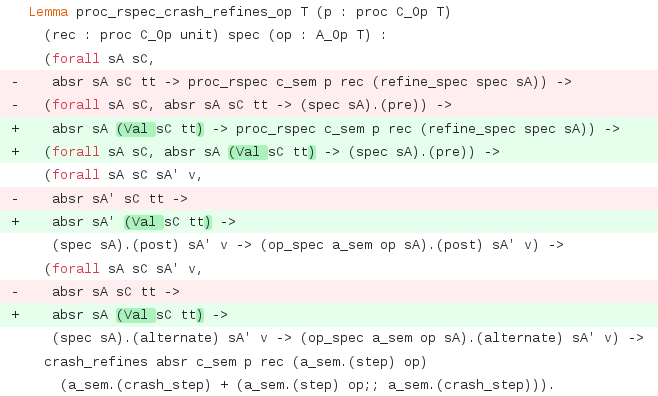
\includegraphics[width=0.47\textwidth]{maintenance/fig/patch.png}
  \caption{Patches to a lemma in User 3, Session 73.}
  \label{fig:patch}
\end{figure}

Figure~\ref{fig:patch} shows an example change patching the arguments
of a lemma. This change wraps two arguments into a single application
in three different hypotheses of a lemma.

\paragraph{Benchmark 6}

11 of the 13 patches to arguments that we found for User 3,
including the example in \Cref{fig:patch}, came from Session 73.
All of these changes similarly wrapped arguments into an application of
\lstinline{Val}.
We suspect that this was due to a change in the definition of \lstinline{absr},
but we were not able to confirm this since
the change in question occurred before the beginning of the study.
The user admitted or aborted the proofs of four of the five
changed lemmas.

\iffalse
For the same reason, we were not able to determine with certainty
that the changes to proofs in that session were corresponding
repairs to match the new specification.
\fi

\paragraph{Benchmark 7}

28 of the 29 replace function changes that we found for User 8
were changes from \lstinline{=} to \lstinline{==} over
the course of about a week in Sessions
2, 14, 37, 40, 65, 79, 108, 125, and 160.
The corresponding proof attempts suggest that while these terms were well-founded with \lstinline{=}, the changes to use \lstinline{==}
may have been necessary to make progress in proofs
using certain tactics.
Sometimes, after making these changes, User 8 also fixed tactics
that had worked before.

\paragraph{Lessons for Automation}

Automation may help with these sorts of repairs to theorems
and proofs. The proof repair tool \textsc{PUMPKIN PATCH} already handles some
repairs to proofs after changes to both
\textbf{Content}~\cite{Ringer2018} and \textbf{Structure}~\cite{Ringer2019}, but has support for repairing the theorem statement itself only in
the latter case, and only for a specific class of changes to inductive types.
These changes provide examples where changing the theorem type is also
desirable, and may make good benchmarks for further development
to support this.

\begin{displayquote}
  \textbf{Takeaway}:
  Proof repair tools should repair programs and specifications,
  not just proofs.
\end{displayquote}

\subsubsection{Interactive Discovery of Programs and Specifications}
\label{sec:pat4}

In Q1 (Section~\ref{sec:q1}), we found that users most often fixed
proofs by stepping up outside of proofs and changing other things.
Our observations from Q2 are consistent with this,
and give some insight into the details.
Changes from Users 3, 7, 8, and 10 all revealed a pattern of interactive
discovery of programs and specifications:
In some cases, these users discovered bugs in their programs during a
proof attempt or test.
In other cases, these users discovered that their specifications were
incorrect, too weak, or difficult to work with.
Users sometimes assigned temporary names to lemmas or theorems,
then renamed them only after finalizing their types.
Even experts made mistakes in programs and theorem statements
(perhaps they were the ones catching them most effectively).

\begin{figure}
  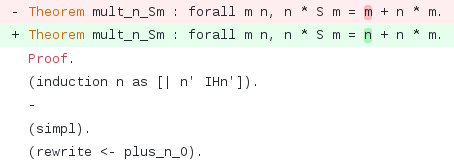
\includegraphics[width=0.35\textwidth]{maintenance/fig/bad.png}
  \caption{A partial attempt at proving and later correction to an incorrect theorem from User 3, Session 11377 (tactic formatting is not preserved in the data
that \toolname receives).}
  \label{fig:bad}
\end{figure}

Figure~\ref{fig:bad} shows an example of catching a bug in a specification
during an attempted proof attempt. The theorem
before the change is impossible (let \lstinline{m} be \lstinline{3} 
and \lstinline{n} be \lstinline{1}).
After attempting to prove it and reaching this goal:

\begin{lstlisting}
  m : nat
  --------
  0 = m
\end{lstlisting}
the user steps up and fixes the theorem statement by replacing an argument
(\textbf{Rpl} \textbf{Arg}), then later finishes the proof.

\paragraph{Benchmark 8}

The change from \Cref{fig:bad} can be found in User 3, Session 11377.
The same session contains changes to the same theorem by
moving arguments (\textbf{Mov} \textbf{Arg}).
The user succeeded at the proof after about three minutes.
%All of the changes moving arguments that we found for User 3
%corresponded to interactive discovery of fixpoints and theorems.

\paragraph{Benchmark 9}

In Session 13, commit 11, User 10 patched a case (\textbf{Pch} \textbf{Cas})
of a fixpoint \lstinline{fib'} after testing.
This took the user about thirty seconds.
The fixpoint \lstinline{fib'} itself may have been used to 
test a different function.

\paragraph{Benchmark 10}

User 7 mainly demonstrated this pattern through
adding and moving hypotheses (\textbf{Add} and \textbf{Mov} \textbf{Hyp}).
The latter most often
corresponded to generalizing the inductive hypothesis 
after a partial proof attempt by swapping theorem hypotheses,
in some cases in order to induct over a different hypothesis 
altogether.
We found such changes in Sessions 19, 56, 93, 94, 104, 110,
153, 159, and 176.
See, for example, \lstinline{match_ty__value_type_l} in Session 94,
commit 15.

\paragraph{Benchmark 11}

In Session 2, User 7 temporarily named a lemma
\lstinline{weird_trans}, then renamed it to \lstinline{sub_r_nf__trans}
by Session 10 after finalizing its type after several partial
proof attempts over the course of about a day and a half.

\paragraph{Lessons for Automation}

The effect of discovering bugs by attempting a proof accounts for some
of the benefits of verification~\cite{murraybp}.
It makes sense, then, to continue to build automation to support users
in finding and fixing those bugs.
One possible unexplored avenue for this is integrating repair tools
with QuickChick~\cite{Paraskevopoulou2015} for testing specifications,
or with the \lstinline{induct} tactic from FRAP~\cite{FRAPBook}
or the hypothesis renaming functionality from CoqPIE~\cite{Roe2016}
for simple generalization of inductive hypotheses.
Integrating tools for discovering lemma and theorem names~\cite{Aspinall2016b}
during the development process may help users who use temporary names.
Above all, repair is not just something that happens to stable proof
developments---change is everywhere in developing those programs and
proofs to begin with.

\begin{displayquote}
  \textbf{Takeaway}: Integrating tools for proof repair with tools
  for discovery and development of specifications
  is an unaddressed opportunity to support proof engineers.
\end{displayquote}


%\section{Conclusions \& Future Work}
\label{sec:discussion}

We built \toolname, a Coq plugin that remotely collects fine-grained
proof development data in a way that is decoupled from the UI.
Using \toolname, we collected data on changes to proofs, programs,
and specifications at a level of granularity not previously
seen for an ITP.
Visualization and analysis of this data revealed evidence in our study
population of development patterns, at times confirming folk knowledge---like 
that discovering  the correct program or specification was often a
conversation with the proof itself, even for experts---and providing
useful insights and benchmarks for tools.

The infrastructure that we have built and the data that we have collected
using it are publicly available.
We hope to see it used as benchmarks for the improvement of
proof engineering tools, and as data for future studies.
We hope to see the infrastructure that we have built reused or
adapted to other ITPs for future studies.

\paragraph{Three Wishes}
We would like for our experiences building and using \toolname
to help the community conduct more studies of proof development processes.
We thus conclude with three wishes, the fulfillment of which would help
address the challenges that we encountered along the way:

\begin{enumerate}
\item Better abstraction of user environments (Section~\ref{sec:wish1})
\item More information about user interaction (Section~\ref{sec:wish2})
\item More users (Section~\ref{sec:wish3})
\end{enumerate}
We discuss how to grant each wish both at the level of study design
and at the level of ITP design in order to facilitate future studies of 
this kind.

\subsection{Wish: Better Abstraction of User Environments}
\label{sec:wish1}

In order to cast as broad of a net as possible for potential users, we
designed \toolname to be independent of the UI, 
the version of Coq, and the build system. Coq's plugin infrastructure
and interaction model offered a promising avenue for this,
%Together with the Coq developers, we were able to extend the plugin API
%with a hook to listen to Coq's REPL.
and Coq's resource file infrastructure meant that users could load the plugin
universally with just one LOC in one location.
All of this gave us the impression of independence from the details of
the UI, ITP version, and build system.

We later found that, while this infrastructure was useful,
the impression of total independence was somewhat of an illusion; 
all of these details mattered.
In particular, while \toolname itself was UI-independent, the analyses
that we ran did not achieve full independence.
For example, we found that depending on the version of Coq and what
event triggers a cancellation, different UIs use different mechanisms
for cancellation (recall these mechanisms from Section~\ref{sec:plugin}). 
Our analyses had to deal with all of these mechanisms.

In addition, partway through the study, we received a bug 
report that noted that one common build system for Coq compiles files by
default using a flag that disables loading the Coq resource file.
This is one possible explanation for the lack of data that some users sent.
To remedy this, we must ask future users of \toolname
to compile all of their Coq projects without using this flag;
we have updated the \toolname documentation to account for this. 

\paragraph{The Study Designer} Without help from the ITP designer,
the study designer cannot achieve full abstraction from these details.
The study designer may, however, work around the lack of full abstraction.
We recommend testing the study infrastructure with 
many different environments for many different scenarios.
It may help to identify potential users early and survey their
development environments before even beginning to test,
covering likely scenarios in advance.
It may also help to build in a short trial period on the final users
before the final data collection begins, thereby
covering their particular development environments.
The latter has the additional benefit of giving the study designer
time to discover and discuss with users possible confounding
variables for analysis, like development style or project phase.

We had the foresight to test \toolname with \lstinline{coqtop}, 
Proof General, and CoqIDE, but we did not anticipate User 5's custom
UI, which treated failures differently from the others.
We also did not anticipate the behavior of different
build systems on Coq's resource file, since we tested only one
build configuration.
We could have avoided both of these issues with our recommendations.
Instead, we had to work around both issues after deployment.

\paragraph{The ITP Designer} 
Most of the power to grant this wish is in the hands of the ITP designer.
Full abstraction over development environments may not be possible, but the
ITP designer may design the interaction model with this as a goal.
The REPL and state machine already strive for this---and come
close to achieving it---but their current implementations in Coq fall short.
Improvements to abstraction here may be minimal, like
providing fewer mechanisms for UIs to accomplish the same thing,
or providing a way to guarantee that a plugin is always loaded for all
build systems.

For a more radical approach, the ITP designer may look to other 
interaction models.
For example, Isabelle/HOL has recently moved away from its REPL,
instead favoring the Prover IDE (PIDE)~\cite{Wenzel2012} framework
as its interaction model.
With PIDE, UIs and ITPs communicate using an asynchronous protocol to manage
versions of a document~\cite{Wenzel2014}, annotating the document with 
new information when it becomes available~\cite{Wenzel2012}.
Personal communication suggests that there is an ongoing attempt to 
to centralize functionality like the build system into PIDE.
While centralization may limit the potential for customization by different
UIs, it may make studies of fine-grained proof development data easier,
since the instrumentation may occur at a higher level,
guaranteeing more uniform interaction.

\subsection{Wish: More Information about User Interaction}
\label{sec:wish2}

By observing state machine messages through the plugin API,
we were able to log data at high enough granularity to reconstruct
hundreds of interactive sessions. This helped us identify incremental
changes to tactics and terms that are difficult to gather from other sources.

The hooks that we designed together with the Coq developers, however, 
were not perfect.
There was no way for us to use those hooks to listen to the messages
that Coq sent back to the UI.
Making this change would have required modifying Coq again, and by the time
we realized this, it was too late.
Listening to those responses would have given us more insight into user
behavior.
It would have also helped us distinguish between failures and stepping up.
Instead, we had to distinguish between these using IDE-specific heuristics,
which left us with no automatic way to distinguish failures from stepping up
for User 5's custom UI.

We also found that once we had collected granular data, 
analyzing it was sometimes difficult. 
For example, sometimes users defined a term, stepped up and changed
an earlier term, then stepped back down and changed the original term.
For such a change, our visualization script constructed 3 consecutive commits;
to determine that the original term had changed, we had to look at 
the difference between the 1st and the 3rd commits.
Sometimes, changes occurred over tens of commits, or over several sessions.
Thus, manual analysis of changes for Q2 was tedious, and involved
not only inspecting thousands of diffs but also understanding each 
session well enough to track term information over time.

We considered automating the analysis for Q2, but we found
automatically classifying changes in terms to be prohibitively difficult.
While part of this was due to the inherent difficulty of the problem,
part of this was also due to missing information:
When the UI backed up to an earlier state, we did not know what was below 
the command or tactic corresponding to that state in the file. 
So, when a user copied and pasted a term and then modified both versions,
or made several changes at once to a term before stepping 
down below it, even manually deciding whether it was the same term 
that had changed or a new term entirely proved to be difficult.

\paragraph{The Study Designer}
To grant this wish, we recommend that the study designer run a beta test, complete with analysis, as we did---and that they do so early,
as we did not.
That way, there is enough time to address needs discovered during testing,
for example by communicating with ITP designers.
It may also help to use multiple methods for data collection,
for example by augmenting the collected data with information from the IDE
to track the state of definitions in the file below the location to
which the user has stepped.

The beta testing phase was extremely useful to us; as a result we
reworked our server infrastructure to receive and easily
analyze larger amounts of data, and we tested data backup
infrastructure and network failure resilience code. 
We also discovered and reported a 
bug\footnote{\url{http://github.com/coq/coq/issues/8989}} in CoqIDE and 
Proof General that had made it impossible for us to tell which 
sessions corresponded to which files; the fix was marked as critical 
and backported to Coq 8.9, so only the analyses for Users 5 (custom UI), 8 (Coq 8.8), and 10 (Coq 8.8) were impacted.
However, while we discovered the lack of response information in the plugin hooks
during this period, we did not have enough time to coordinate with Coq developers on
changes to the hooks. 
Leaving more time between testing and the final study would have helped us.

\paragraph{The ITP Designer} 
By implementing hooks like the one that we helped implement for Coq,
the ITP designer can make it easier for researchers to study 
proof development processes. 
To grant this wish, we recommend that these hooks expose not just 
request information, but also response information, 
especially error information.

Augmenting the interaction model with more information
about the file may also help.
For example,
the interaction model could expose a simple and uniform way for UIs
to track that a definition in a new state corresponds to a definition 
in a previous state (that is, that the user did not remove that
definition from the file and replace it with something entirely new). 
This could make it much simpler for an analysis to track changes to a definition over time,
and to choose the granularity with which to inspect changes.
There is some tension between this and the wish for abstraction from
Section~\ref{sec:wish1}, but it may be worth weighing the tradeoffs.

\subsection{Wish: More Users}
\label{sec:wish3}

We attempted to recruit a large and representative sample of Coq proof
engineers.
In our attempts to recruit users, we contacted programming
languages groups at several universities that were known to be working
with Coq, and emailed \lstinline{coq-club} with our project
pitch. We included a promotional video in the hopes of
attracting as many users as possible.

In the end, however, we were able to recruit only 12 users,
all of whom were intermediate through expert users with at least two years
of Coq experience. We received interactive sessions for just 8 of 12
of these users. While this data was rich and granular, with just 8 users,
we were not able to reach broad conclusions about proof engineers more generally.

Part of this was likely due to the demographics of the
community: Compared to other programming environments,
Coq has only a small number of users,
many of whom have or are pursuing graduate degrees.
However, part of this may have been due to
deterrents in our screening process, or poor incentives for our users.

\paragraph{The Study Designer}
The study designer may fulfill this in part by casting as broad of a net
as possible, carefully considering any deterrents in screening criteria.
It may help to use welcoming language to encourage potential users
who are unsure if they qualify.
To reach beginner users, it may help to recruit students.
To reach a more international audience, it may help to distribute
promotional materials and consent forms in multiple languages.
It may also help to consider incentives that appeal to proof engineers.
However, until the ITP user community grows significantly, it will continue 
to be difficult to conduct large-scale studies of proof engineering.

We reached users from different institutions, but
most of our users had similar levels of expertise. We suspect that this was
in part because we asked for users to have at least a year of 
experience using Coq, so as to avoid mixing in data from
users learning Coq for the first time.
We also required fluency in English to ensure that users understood
the consent forms.
Both of these may have deterred users.
One potential user who did not participate noted that we did not make
it clear in our recruitment materials that data from occasional rather
than frequent Coq users was still useful to us.
The same potential user noted that we could have engaged more
with community leaders, thereby giving others in the community
more incentive to participate.
We considered monetary incentives, but ultimately decided they were less
tempting to the community than appeals to improving tools.
Perhaps this was misguided or attracted a more advanced population,
and perhaps we could have considered a different incentive.

\paragraph{The ITP Designer}
The ITP designer may help reduce the costs of participating in these studies. 
We suspect that the primary gains here will come from continuing to 
break down barriers to using plugins and other outside tooling. 
Some examples of this include reducing the brittleness of plugin APIs 
over time, improving build and distribution systems, making it possible 
to prove that a plugin does not interact with a kernel in a way that 
could compromise soundness of the system, 
and providing more support for users who port proof developments
and tools between ITP versions.

Of course, continuing to improve the ITP itself may continue 
to expand the community to reach more users. 
This may cause a positive feedback loop, helping to collect more data 
in order to drive further improvements to the ITP, in turn continuing to help
the community grow.




%\chapter{Related Work}

% TODO whatever else isn't here yet, and some of this might be factored out or partially factored out---all papers, including survey, plus generals

\section{Programs}

\subsection*{Program Refactoring} 

Refactoring~\cite{Mens:2004:SSR:972215.972286}.

\subsection*{Program Repair} 

% From PUMPKIN PATCH, unchanged

Adapting proofs to changes is essentially program repair
for dependently typed languages. 
Program repair tools for 
languages with non-dependent type 
systems~\cite{Pei:2014:APR:2731750.2731779, Long:2016:APG:2837614.2837617, Le:2017:SSS:3106237.3106309, Mechtaev:2016:ASM:2884781.2884807, Monperrus2015} 
may have applications in the context of a dependently typed language.
Similarly, our work may have applications within program repair in these languages:
Future applications of our approach may repurpose it to repair programs for functional languages.

\subsection*{Ornaments}

% From PUMPKIN PATCH, unchanged

Ornaments~\cite{Dagand17jfp, Williams:2014:OP:2633628.2633631}
separate the computational and logical components of a datatype, and may
make proofs more resilient to datatype changes.

\subsection*{Programming by Example}

% From PUMPKIN PATCH, unchanged

Our approach generalizes an example that the programmer provides.
This is similar to programming by example, a subfield of 
program synthesis~\cite{DBLP:journals/ftpl/GulwaniPS17}. 
This field addresses different challenges in different logics,
but may drive solutions to similar problems in a dependently typed language.

\subsection*{Differencing \& Incremental Computation}

% From PUMPKIN PATCH, unchanged

Existing work in differencing and incremental computation may help 
improve our semantic differencing component.
Type-directed diffing~\cite{Miraldo:2017:TDS:3122975.3122976}
finds differences in algebraic data types.
Semantics-based change impact analysis~\cite{Autexier:2010:SCI:1860559.1860580} models semantic differences
between documents.
Differential assertion checking~\cite{differential-assertion-checking-2} analyzes different
versions of a program for relative correctness with respect to a specification.
Incremental $\lambda$-calculus~\cite{Cai:2014:TCH:2594291.2594304} introduces a general model for program changes.
All of these may be useful for improving semantic differencing.

\section{Proofs}

\subsection*{Proof Reuse}

% From PUMPKIN PATCH, unchanged

Our approach reimagines the problem of proof reuse in the context of proof automation.
While we focus on changes that occur over time, traditional proof reuse techniques can help
improve our approach.
Existing work in proof reuse focuses on transferring proofs between isomorphisms,
either through extending the type system~\cite{Barthe:2001:TIP:646793.704711} or through an automatic method~\cite{Magaud2002}.
This is later generalized and implemented in Isabelle~\cite{Huffman2013} and Coq~\cite{ZimmermannH15, tabareau:hal-01559073};
later methods can also handle implications. 
%Transfer tactics apply these functions but do not infer them, while our approach
%infers these functions but does not apply them.
Integrating a transfer tactic with a proof patch finding tool will create an end-to-end
tool that can both find patches and apply them automatically.

Proof reuse for extended inductive types~\cite{Boite2004} adapts proof obligations
to structural changes in inductive types. Later work~\cite{Mulhern06proofweaving} proposes a method
to generate proofs for new constructors. These approaches may be useful when extending the differencing
component to handle structural changes. Existing work in theorem reuse and proof generalization~\cite{Felty1994, pons00, Johnsen2004} abstracts existing proofs for reusability, and may be useful
for improving the abstraction component.
Our work focuses on the components critical to searching for patches; these complementary approaches
can drive improvements to the components.

\subsection*{Proof Evolution}

% From PUMPKIN PATCH, unchanged

There is a small body of work on change and dependency management for verification,
both to evaluate impact of potential changes and maximize reuse~\cite{873647, Autexier:2010:CMH:1986659.1986663}
and to optimize build performance~\cite{Celik:2017:IRP:3155562.3155588}.
These approaches may help isolate changes, which is necessary to identify future benchmarks, integrate
with CI systems, and fully support version updates.

\subsection*{Proof Refactoring}

\subsection*{Proof Repair}

\subsection*{Proof Design}

% From PUMPKIN PATCH, unchanged:

Existing proof engineering work addresses brittleness
by planning for changes~\cite{proof-eng} and designing theorems and proofs that make maintenance less of an issue.
Design principles for specific domains (such as formal metatheory~\cite{Aydemir2008, Delaware2013POPL, Delaware2013ICFP})
can make verification more tractable. CertiKOS~\cite{certikos} introduces the idea of a deep specification to
ease verification of large systems.
These design principles and frameworks are complementary to our approach.
Even when programmers use informed design principles,
changes outside of the programmer's control can break proofs;
our approach addresses these changes.

\subsection*{Proof Automation}

% From PUMPKIN PATCH, unchanged:

We address a missed opportunity in proof automation for ITP: searching
for patches that can fix broken proofs.
This is complementary to existing automation techniques. Nonetheless, there is a wealth
of work in proof automation that makes proofs more resilient to change.
Powerful tactics like \lstinline{crush}~\cite{chlipala:cpdt} can make
proofs more resilient to changes. 
Hammers like Isabelle's sledgehammer~\cite{Blanchette2013} can make proofs agnostic to some low-level changes.
Recent work~\cite{coqhammer} paves the way for a hammer in Coq.
Even the most powerful tactics cannot address all changes;
our hope is to open more possibilities for automation.

Powerful project-specific tactics~\cite{chlipala:cpdt, Chlipala2013} can help prevent low-level maintenance tasks.
Writing these tactics requires good engineering~\cite{Gonthier2011} and domain-specific knowledge,
and these tactics still sometimes break in the face of change.
A future patching tool may be able to repair tactics; the debugging process
for adapting a tactic is not too dissimilar to providing an example to a tool.

Rippling~\cite{rippling} is a technique for automating inductive proofs that uses restricted rewrite rules to
guide the inductive hypothesis toward the conclusion; this may guide improvements to the
differencing, abstraction, and specialization components.
The abstraction and factoring components address specific classes of unification problems;
recent developments to higher-order unification~\cite{Miller:2012:PHL:2331097} may help
improve these components.
Lean~\cite{selsam:lean} introduces the first congruence closure algorithm for dependent type theory that
relies only on the Uniqueness of Identity Proofs (UIP) axiom. While UIP is not fundamental to Coq,
it is frequently assumed as an axiom; when it is, it may be tractable to use a similar algorithm to improve the tool.

GALILEO~\cite{bundyreasoning} repairs faulty physics theories
in the context of a classical higher-order logic (HOL); there is preliminary work extending this
style of repair to mathematical proofs. 
Knowledge-sharing methods~\cite{tgck-cicm14} can adapt some proofs across different representations of HOL.
These complementary approaches may guide extensions to support decidable domains and classical logics.

\subsection*{Transport}

\subsection*{Parametricity}

\subsection*{Refinement}





\section{Proof Repair}
\label{sec:mot-rep}

Name inspired by program repair, but quite different as we'll soon see.

Recall thesis: Changes in programs, specifications, and proofs carry information that a tool can extract, generalize, and apply to fix other proofs broken by the same change. A tool that automates this can save work for proof engineers relative to reference manual repairs in practical use cases.

Proof repair accomplishes this using a combination of differencing and program transformations.

Differencing extracts the information from the change in program, specification, or proof.

The transformations then generalize that information to a more general fix for other proofs broken by the same change.

The details of applying the fix vary by the kind of fix, as we'll soon see.

Crucially, all of this happens over the proof terms in this rich language we saw in the Development section. This is kind of the key insight that makes it all work.

This is great because this language gives us so much information and certainty. This helps us with two of the biggest challenges from program repair. (generals related work)

But it's also challenging because this language is so unforgiving. Plus, in the end, we need these tactic proofs, not just proof terms. So we can't just reuse program repair tools. (generals related work)

So next two chapters will show two tools in our tool suite that work this way, how they handle these challenges, and how they save work.



\section{Approach}

In the example from Section~\ref{sec:patch-motivating}, the example change in one proof carries enough information
to fix other proofs broken by the same change (namely the rewrite by \lstinline{INR\_IPR}).
So a tool can extract that, generalize it, and use it to fix other proofs broken by the same change.
\sysname takes advantage of this more generally.

To use \sysname (Section~\ref{sec:pumpkin-workflow}), the proof engineer modifies a single proof script to provide an \textit{example} of how to adapt a proof to a change.
\sysname extracts that information into a \textit{patch candidate}---which is localized to the context of the example, but not enough to fix other proofs broken by the change.
It then generalizes that candidate into a \textit{reusable patch}: a function
that can be used to fix other broken proofs broken by the same change, which \sysname defines as a Coq term.
In other words, looking back to the thesis statement, the information shows up in the difference between versions of the example patched proof.
\sysname can extract and generalize that information.

\sysname focuses in particular on searching for patches to proofs that break in response changes in the \textit{content}, but not the \textit{structure}
of programs and specifications (Section~\ref{sec:pumpkin-scope}).
As mentioned earlier, \sysname does this using a combination of semantic differencing and proof term transformations.
Differencing (Section~\ref{sec:pumpkin-spec-diff} looks at the difference between versions of the example patched proof for this information, and finds the candidate.
Then, proof term transformations (Section~\ref{pumpkin-spec-trans}) modify that candidate to produce the reusable proof patch.
And of course all of this happens over proof terms, since tactics might hide necessary information
(example before didn't show this, but example here will).
For now, support for both proof scripts and patch application is simple (see Section~\ref{sec:TODO}), though both of these are addressed in Chapter~\ref{sec:TODO}.

\subsection{Workflow: Patching by Example}
\label{sec:pumpkin-workflow}

\begin{figure}
%\begin{algorithm}
\begin{algorithmic}
\renewcommand{\thealgorithm}{}
\footnotesize
\caption{\footnotesize{find\_patch(term, term', direction)}}
    \STATE \diff{\textit{diff} types of term and term' for goals}
    \STATE \diff{\textit{diff} term and term' for candidates}
    \IF{there are candidates}
      \STATE \diff{\textit{factor}, \textit{abstract}, \textit{specialize}, and/or \textit{invert} candidates}
      \IFRETURN{there are patches}{patches}
    \ENDIF
    \RETURN failure
\end{algorithmic}
%\end{algorithm}
\caption{Search procedure for a reusable proof patch in \sysname.}
\label{alg:patching}	
\end{figure}

\sysname exposes a \lstinline{Patch Proof} command that invokes the proof patch search procedure in Figure~\ref{alg:patching}.
\lstinline{Patch Proof} takes as input the old and new version of an example proof patched in response to some breaking change.
When succesful, it returns the reusable proof patch as a function, and defines it in Coq.
There are some limitations in scope described partially here and partially in the repository.
The \sysname repository also contains a detailed user guide.
Options described in the implementation section make it possible to automate application to some degree as well if desired,
and the implementation describes a lot more, too.

% New (outline for now), plus parts of PUMPKIN PATCH Motivating the Core

\begin{figure*}
\begin{minipage}{0.50\textwidth}
\lstset{language=coq, aboveskip=0pt, belowskip=0pt}
\lstinputlisting[firstline=1, lastline=1]{repair/introex.tex}
\lstinputlisting[backgroundcolor=\color{orange!35},firstline=2,lastline=2]{repair/introex.tex}
\lstinputlisting[firstline=3, lastline=8]{repair/introex.tex}
\lstinputlisting[firstline=1, lastline=4]{repair/introexterm.tex}
\lstinputlisting[backgroundcolor=\color{orange!35},firstline=5,lastline=5]{repair/introexterm.tex}
\lstinputlisting[firstline=6, lastline=9]{repair/introexterm.tex}
\end{minipage}
\hfill
\begin{minipage}{0.48\textwidth}
\lstset{language=coq, aboveskip=0pt, belowskip=0pt}
\lstinputlisting[firstline=9, lastline=9]{repair/introex.tex}
\lstinputlisting[backgroundcolor=\color{orange!35},firstline=10,lastline=10]{repair/introex.tex}
\lstinputlisting[firstline=11, lastline=16]{repair/introex.tex}
\lstinputlisting[firstline=11, lastline=14]{repair/introexterm.tex}
\lstinputlisting[backgroundcolor=\color{orange!35},firstline=15,lastline=15]{repair/introexterm.tex}
\lstinputlisting[firstline=16, lastline=19]{repair/introexterm.tex}
\end{minipage}
\caption{Two proofs with different conclusions (top) and the
corresponding proof terms (bottom) with relevant type information. We highlight the change in theorem conclusion and
the difference in terms that corresponds to a patch.}
\label{fig:example}
\end{figure*}

% TODO list of configurations supported?
The specifics of this procedure vary by the particular class of change.
\sysname infers a \textit{configuration} from the example change.
This configuration customizes the highlighted lines for an entire class of changes:
It determines what to diff on lines 1 and 2,
and what transformations to run to achieve what goal on line 4.
There are four transformations that turn patch candidates into reusable proof patches:

\begin{enumerate}
\item \textit{Patch specialization} to arguments
\item \textit{Patch abstraction} of arguments or functions
\item \textit{Patch inversion} to reverse a patch
\item \textit{Lemma factoring} to break a term into parts
\end{enumerate}
The configuration chooses among these strategically based on the structure of the proof term.

To motivate this workflow, consider using \sysname to search the proofs in
Figure~\ref{fig:example} for a patch between conclusions.
Except we will show a place where the lemma is actually applied.
Note that the tactics don't change even though the terms do---and even though the change could break other proofs.

So what do we do?
We invoke the plugin using \lstinline{old} and \lstinline{new} as the example change:

\begin{lstlisting}[language=ml4]
  Patch Proof old new as patch.
\end{lstlisting}

The first thing that \sysname does is determine the configuration.
Here, it uses the configuration for changes in conclusions of two proofs
that induct over the same hypothesis. Given two such
proofs:

%We describe one
%such procedure in this section; we descibe three more
%in Section~\ref{sec:case}.
\begin{lstlisting}[language=coq]
  (@\ltacforall@) x, H x $\rightarrow$ (@\diff{P}@) x(@\vspace{-0.1cm}@)
  (@\ltacforall@) x, H x $\rightarrow$ (@\diff{P'}@) x
\end{lstlisting}
\sysname searches for a patch with this type:

\begin{lstlisting}[language=coq]
  (@\ltacforall@) x, H x $\rightarrow$ (@\diff{P'}@) x $\rightarrow$ (@\diff{P}@) x
\end{lstlisting}
using this configuration:

\begin{algorithm}
\footnotesize
\begin{algorithmic}[1]
%  Is it really necessary to say that an algorithm might do initialization?
%  \STATE Build trees for search
  %\STATE build trees for proofs
  %\REPEAT
    \STATE \textit{diff} conclusion types for goals
    \STATE \textit{diff} conclusion terms for candidates
    \STATE \textbf{if} there are candidates \textbf{then}
    \STATE \hspace*{1em} \textit{abstract} and then \textit{specialize} candidates
\end{algorithmic}
\end{algorithm}

When it runs the procedure,
\sysname first determines the type that a patch from \lstinline{new} to \lstinline{old} should have.
To determine this, it semantically \textit{diffs} the types and finds this goal type:

\begin{lstlisting}[language=coq]
  (@\ltacforall@) n m p, n <= m $\rightarrow$ m <= p $\rightarrow$ (@\diff{n <= p}@) $\rightarrow$ (@\diff{n <= p + 1}@)
\end{lstlisting}
It then breaks each inductive proof into cases and determines an intermediate goal type for the candidate.
%recursively searches each case for a candidate.
In the base case, for example, it \textit{diffs} the types and determines that a candidate
between the base cases of \lstinline{new} and \lstinline{old} should have this type (lines 11 and 12):

\begin{lstlisting}
  (@\diff{(fun p0 => n <= p0)}@) m $\rightarrow$ (@\diff{(fun p0 => n <= p0 + 1)}@) m
\end{lstlisting}
It then \textit{diffs} the terms (line 13) for such a candidate:

\begin{lstlisting}
  fun n m p H0 H1 =>(@\vspace{-0.04cm}@)
    (fun (H : n <= m) => (@\diff{le\_plus\_trans n m 1}@) H)(@\vspace{-0.04cm}@)
  : (@\ltacforall@) n m p, n <= m -> m <= p -> (@\diff{n <= m}@) -> (@\diff{n <= m + 1}@)
\end{lstlisting}

This candidate is close, but it is not yet a patch. This candidate
maps base case to base case (it is applied to \lstinline{m}); the patch should map conclusion to conclusion (it should
be applied to \lstinline{p}).

Here, \sysname \textit{abstracts} this candidate by \lstinline{m} (line 11), which lifts it out of the base case:

\begin{lstlisting}
  fun (@\diff{n0}@) n m p H0 H1 =>(@\vspace{-0.04cm}@)
    (fun (H : n <= (@\diff{n0}@)) => le_plus_trans n (@\diff{n0}@) 1 H)(@\vspace{-0.04cm}@)
  : (@\ltacforall@) (@\diff{n0}@) n m p, n <= m -> m <= p -> n <= (@\diff{n0}@) -> n <= (@\diff{n0}@) + 1
\end{lstlisting}
\sysname then \textit{specializes} this candidate to \lstinline{p} (line 16), the argument
to the conclusion of \lstinline{le_ind}. This produces a patch:

\begin{lstlisting}
  patch n m p H0 H1 := (@\vspace{-0.04cm}@)
    (fun (H : n <= (@\diff{p}@)) => le_plus_trans n (@\diff{p}@) 1 H)(@\vspace{-0.04cm}@)
  : (@\ltacforall@) n m p, n <= m $\rightarrow$ m <= p $\rightarrow$ n <= (@\diff{p}@) -> n <= (@\diff{p}@) + 1
\end{lstlisting}
The user can then use \lstinline{patch} to fix other broken proofs.
For example, given a proof that applies \lstinline{old}, the user can use \lstinline{patch} to prove the same conclusion
by applying \lstinline{new}:

\begin{lstlisting}[language=coq]
  (@\succeeds{apply old.}@)(@\vspace{-0.1cm}@)
  (@\diff{apply patch.}@) (@\succeeds{apply new.}@)
\end{lstlisting}
This can happen automatically through hint databases.

This simple example uses only two transformations. The other transformations help turn candidates
into patches in similar ways. We discuss all of this in detail later.
Later we will see real-world examples that demonstrate more configurations, too.
For now let's talk about the scope more.

\subsection{Scope: Changes in Content}
\label{sec:pumpkin-scope}

% TODO somewhere distinguish between prototype and suite of tools meaningfully
The 2018 \sysname prototype searches for patches to proofs broken by changes in the content of programs and specifications.
The corresponding differencing algorithms run in response to a breaking change in the content of a program or specification. % TODO clarify ``certain''?
They focus in particular on changes that do not add, remove, or rearrange any assumptions.
Chapter~\ref{TODO} explains an extension to \sysname that supports a broad class of
changes in datatypes that may change in those ways.

Basically the main barrier here is that this produces a function that the user must apply.
Thus it can't handle changes that move things around, as these need to be transformed directly.
Mention the particular configurations implemented here honestly, but then note that general approach is cool when it produces a function.

\subsection{Differencing: Candidates from Examples}
\label{sec:pumpkin-spec-diff}

Differencing takes as inputs $\ldots$ and returns $\ldots$:

\begin{itemize}
\item \textbf{Inputs}: $\ldots$, assuming:
\begin{itemize}
\item $\ldots$
\end{itemize}
\item \textbf{Outputs}: $\ldots$, guaranteeing:
\begin{itemize}
\item $\ldots$
\end{itemize}
\end{itemize}

other details like what is proven or whatever (here, maybe the list of differencing procedures actually supported?)

\iffalse
\paragraph{Input: Example Patched Proof}
They look at the difference between the old and new versions of a single example patched proof in response to that change.
Old and new version of example patched proof.
%\sysname is a proof-of-concept and does not yet handle some kinds of proofs.
%In each scenario, we made minor modifications to proofs so that we could use \sysname (for example,
%using induction instead of destruction).

\paragraph{Output: Patch Candidates}
Functions that map back and forth between the old and new versions
of the example patch proof in a particular context, but do not yet generalize to other contexts.
\fi

\subsection{Transformations: Patches from Candidates}
\label{sec:pumpkin-spec-trans}

The transformations takes as inputs $\ldots$ and return $\ldots$:

\begin{itemize}
\item \textbf{Inputs}: $\ldots$, assuming:
\begin{itemize}
\item $\ldots$
\end{itemize}
\item \textbf{Outputs}: $\ldots$, guaranteeing:
\begin{itemize}
\item $\ldots$
\end{itemize}
\end{itemize}

other details like what is proven or whatever

\iffalse
\paragraph{Input: Patch Candidates}
They come from differencing.

\paragraph{Output: Reusable Proof Patch}
The corresponding proof term transformations then try to transform each of those candidate patch functions to a more general \textit{reusable proof patch}:
a function that can be applied with traditional proof automation to fix other proofs broken by the same change.
\fi



\section{Differencing}
\label{sec:pi-diff}

% TODO explain how this fits into differencing, that differencing can be done by the human or by the tool, and so on

\begin{figure*}
\begin{minipage}{0.48\textwidth}
\begin{lstlisting}
DepConstr(0, list T) : list T := Constr((@\codediff{0}@), list T).(@\vspace{-0.04cm}@)
DepConstr(1, list T) t l : list T :=(@\vspace{-0.04cm}@)
  Constr ((@\codediff{1}@), list T) t l.(@\vspace{-0.04cm}@)
(@\vspace{-0.14cm}@)
DepElim(l, P) { p$_{\mathtt{nil}}$, p$_{\mathtt{cons}}$ } : P l :=(@\vspace{-0.04cm}@)
  Elim(l, P) { (@\codediff{p$_{\mathtt{nil}}$}@), (@\codediff{p$_{\mathtt{cons}}$}@) }.(@\vspace{-0.04cm}@)
\end{lstlisting}
\end{minipage}
\hfill
\begin{minipage}{0.48\textwidth}
\begin{lstlisting}
DepConstr(0, list T) : list T := Constr((@\codediff{1}@), list T).(@\vspace{-0.04cm}@)
DepConstr(1, list T) t l : list T :=(@\vspace{-0.04cm}@)
  Constr((@\codediff{0}@), list T) t l.(@\vspace{-0.04cm}@)
(@\vspace{-0.14cm}@)
DepElim(l, P) { p$_{\mathtt{nil}}$, p$_{\mathtt{cons}}$ } : P l :=(@\vspace{-0.04cm}@)
  Elim(l, P) { (@\codediff{p$_{\mathtt{cons}}$}@), (@\codediff{p$_{\mathtt{nil}}$}@) }.(@\vspace{-0.04cm}@)
\end{lstlisting}
\end{minipage}
\vspace{-0.3cm}
\caption{The dependent constructors and eliminators for old (left) and new (right) \lstinline{list}, with the difference in \codediff{orange}.}
\vspace{-0.1cm}
\label{fig:listconfig}
\end{figure*}

Differencing---whether done by the tool (automatic configuration) or by the proof engineer (manual configuration)---identifies 
and proves a type equivalence. But differening further decomposes that equivalence into a form called a \textit{configuration}. 
The configuration is the key to building a proof term transformation that implements transport in a way that is suitable for repair.

Each configuration corresponds to an equivalence \Aa $\simeq$ \B.
It deconstructs the equivalence into things that talk about \Aa, and things that talk about \B.
It does so in a way that hides details
specific to the equivalence, like the order or number of arguments to an induction principle or type.

At a high level, the configuration helps the transformation achieve two goals: 

\begin{enumerate}
\item preserve equality up to transport across the equivalence between \Aa and \B (Section~\ref{sec:pi-diff-equiv}), and 
\item produce well-typed terms (Section~\ref{sec:pi-diff-equal}).
\end{enumerate}
To differencing, this configuration is a pair of pairs of terms:

\begin{lstlisting}
  ((DepConstr, DepElim), (Eta, Iota))(@\vspace{-0.05cm}@)
\end{lstlisting}
each of which corresponds to one of the two goals:
\lstinline{DepConstr} and \lstinline{DepElim} define how to transform constructors and eliminators, thereby preserving the equivalence, and 
\lstinline{Eta} and \lstinline{Iota} define how to transform $\eta$-expansion and $\iota$-reduction of constructors and eliminators, thereby producing well-typed terms.

Formally, every correct configuration corresponds to an initial algebra of an endofunctor,
and correctness---that every configurations and equivalences are isomorphic---follows by Lambek's theorem (Section~\ref{sec:art}).\footnote{When I met with Michael Shulman over coffee in San Diego a few years ago, he at various points said that a preliminary version of this work ``feels like univalence,'' ``feels like coherence,'' and ``feels like an endofunctor.'' All three were correct! But I didn't understand the connection to endofunctors by way of Lambek's until a few months before writing this thesis.
Anders M\"{o}rtberg and Carlo Angiuli identified this connection, and Carlo explained it to me in great detail.
It is quite beautiful!}  % TODO
Each search procedure for automatic configuration produces both the configuration and the equivalence that it induces (Section~\ref{sec:proc}).
Manual configuration takes as input the configuration directly.
(Mention Section~\ref{sec:pi-diff-limits} somehow.)

All terms that I introduce in this section are in \kl{CIC$_{\omega}$} with \kl{primitive eliminators}. % TODO point to other conventions again
Section~\ref{sec:pi-diff-limits} describes the limitations, and Section~\ref{sec:pi-implementation} describes how I scale this from CIC$_{\omega}$ to Coq.

\subsection{Preserving the Equivalence}
\label{sec:pi-diff-equiv}

To preserve the equivalence, the configuration maps terms over \Aa to terms over \B by viewing each
term of type \B as if it were an \Aa.
This way, the transformation in Section~\ref{sec:pi-trans} can replace values of \Aa with values of \B, and
inductive proofs about \Aa with inductive proofs about \B, %, then recursively transform
%subterms 
all without changing the order or number of arguments.

The two configuration parts responsible for this are \lstinline{DepConstr}
and \lstinline{DepElim} (\textit{dependent constructors} and \textit{eliminators}).
These describe how to construct and eliminate \Aa and \B, wrapping the types with a common inductive structure.
The transformation requires the same number of dependent constructors and cases in dependent eliminators for \Aa and \B,
even if \Aa and \B are types with different numbers of constructors
(\Aa and \B need not even be inductive; see Sections~\ref{sec:art} and~\ref{sec:pi-results}).

For the \lstinline{list} change from Section~\ref{sec:overview},
the configuration that \toolnamec discovers uses the dependent constructors
and eliminators in Figure~\ref{fig:listconfig}. The dependent constructors for \lstinline{Old.list}
are the normal constructors with the order unchanged,
while the dependent constructors for \lstinline{New.list} swap constructors
back to the original order.
Similarly, the dependent eliminator for \lstinline{Old.list} is the normal eliminator for \lstinline{Old.list},
while the dependent eliminator for \lstinline{New.list} swaps cases.

As the name hints, these constructors and eliminators can be dependent.
Consider the type of vectors of some length:

\begin{lstlisting}
packed_vect T := $\Sigma$(n : nat).vector T n.(@\vspace{-0.05cm}@)
\end{lstlisting}
\toolnamec can port proofs across the equivalence between this type and \lstinline{list T}~\href{https://github.com/uwplse/pumpkin-pi/blob/v2.0.0/plugin/coq/examples/Example.v}{\circled{3}}. % Example.v
The dependent constructors \toolnamec discovers pack the index into an existential, like:

\begin{lstlisting}
DepConstr(0, packed_vect) : packed_vect T :=(@\vspace{-0.04cm}@)
  $\exists$ (Constr(0, nat)) (Constr(0, vector T)).(@\vspace{-0.05cm}@)
\end{lstlisting}
and the eliminator it discovers eliminates the projections:

\begin{lstlisting}
DepElim(s, P) { f$_0$ f$_1$ } : P ($\exists$ ($\pi_l$ s) ($\pi_r$ s)) :=(@\vspace{-0.04cm}@)
  Elim($\pi_r$ s, $\lambda$(n : nat)(v : vector T n).P ($\exists$ n v)) {(@\vspace{-0.04cm}@)
    f$_0$,(@\vspace{-0.04cm}@)
    ($\lambda$(t : T)(n : nat)(v : vector T n).f$_1$ t ($\exists$ n v))(@\vspace{-0.04cm}@)
  }.(@\vspace{-0.05cm}@) 
\end{lstlisting}

In both these examples, the interesting work moves into the configuration:
the configuration for the first swaps constructors and cases,
and the configuration for the second maps constructors and cases over \lstinline{list} to constructors and cases over \lstinline{packed_vect}. %packs constructors and eliminates projections.
That way, the transformation need not add, drop, or reorder arguments---it can truly be generic over type equivalences.
%In essence, all of the difficult work moves into the configuration.
Furthermore, both examples use automatic configuration, so differencing in \toolnamec's \textbf{Configure} component
discovers \lstinline{DepConstr} and \lstinline{DepElim} from just the types \Aa and \B, taking care of even the difficult work.

\subsection{Producing Well-Typed Terms}
\label{sec:pi-diff-equal}

The other configuration parts \lstinline{Eta} and \lstinline{Iota} deal with producing well-typed terms,
in particular by transporting equalities.
CIC$_{\omega}$ distinguishes between two important kinds of equality: those that hold by reduction (\textit{definitional} equality), and those that hold by proof (\textit{propositional} equality).
That is, two terms \lstinline{t} and \lstinline{t'} of type \lstinline{T} are definitionally equal if they reduce to the same normal form,
and propositionally equal if there is a proof that \lstinline{t = t'} using the inductive
equality type \lstinline{=} at type \lstinline{T}. Definitionally equal terms are necessarily propositionally equal, but 
the converse is not in general true. % TODO this should probably go into an earlier section

When a datatype changes, sometimes, definitional equalities defined over the old version of that type must become propositional.
A naive proof term transformation may fail to generate well-typed terms if it does not account for this.
Otherwise, if the transformation transforms a term \lstinline{t : T} to some \lstinline{t' : T'}, it does not necessarily
transform \lstinline{T} to \lstinline{T'}~\cite{tabareau2019marriage}.

\lstinline{Eta} and \lstinline{Iota} describe how to transport equalities.
More formally, they define $\eta$-expansion and $\iota$-reduction of \Aa and \B,
which may be propositional rather than definitional,
and so must be explicit in the transformation.
$\eta$-expansion describes how to expand a term to apply a constructor to an eliminator in a way that preserves propositional equality,
and is important for defining dependent eliminators~\cite{nlab:eta-conversion}.
$\iota$-reduction ($\beta$-reduction for inductive types) describes how to reduce an elimination of a constructor~\cite{nlab:beta-reduction}.

The configuration for the change from \lstinline{list} to \lstinline{packed_vect} has propositional \lstinline{Eta}.
It uses $\eta$-expansion for $\Sigma$:

\begin{lstlisting}
  Eta(packed_vect) := $\lambda$(s:packed_vect).$\exists$ ($\pi_l$ s) ($\pi_r$ s).(@\vspace{-0.05cm}@)
\end{lstlisting}
which is propositional and not definitional in Coq.
Thanks to this, we can forego the assumption that our language has primitive projections (definitional $\eta$ for $\Sigma$).

\begin{figure}
\begin{minipage}{0.44\columnwidth}
   \lstinputlisting[firstline=1, lastline=8]{often/nattobin.tex}
\end{minipage}
\hfill
\begin{minipage}{0.54\columnwidth}
   \lstinputlisting[firstline=10, lastline=17]{often/nattobin.tex}
\end{minipage}
\vspace{-0.2cm}
\caption{A unary natural number \lstinline{nat} (left) is either zero (\lstinline{0}) or the successor of some other natural number (\lstinline{S}).
A binary natural number \lstinline{N} (right) is either zero (\lstinline{N0}) or a positive binary number (\lstinline{Npos}), where a positive binary number is either 1 (\lstinline{xH}), or the result of shifting left and adding 1 (\lstinline{xI}) or
0 (\lstinline{xO}). Unary and binary natural numbers are equivalent, but have different inductive structures.
Consequentially, definitional equalities over \lstinline{nat} may become propositional over \lstinline{N}.}
\vspace{-0.2cm}
\label{fig:nattobin}
\end{figure}

Each \lstinline{Iota}---one per constructor---describes and proves the $\iota$-reduction behavior
of \lstinline{DepElim} on the corresponding case.
This is needed, for example, to port proofs about unary numbers \lstinline{nat} to
proofs about binary numbers \lstinline{N} (Figure~\ref{fig:nattobin}).
While we can define \lstinline{DepConstr} and \lstinline{DepElim} to induce an equivalence
between them~\href{https://github.com/uwplse/pumpkin-pi/blob/v2.0.0/plugin/coq/nonorn.v}{\circled{5}}, % nonorn.v (TODO update links throughout)
we run into trouble reasoning about applications of \lstinline{DepElim},
since proofs about \lstinline{nat} that hold by reflexivity do not necessarily hold by reflexivity over \lstinline{N}. 
For example, in Coq, while \lstinline{S (n + m)  = S n + m} holds by reflexivity over \lstinline{nat},
when we define \lstinline{+} with \lstinline{DepElim} over \lstinline{N},
the corresponding theorem over \lstinline{N} does not hold by reflexivity.

To transform proofs about \lstinline{nat} to proofs about \lstinline{N}, we must transform \textit{definitional} $\iota$-reduction over \lstinline{nat} to \textit{propositional} $\iota$-reduction over \lstinline{N}.
For our choice of \lstinline{DepConstr} and \lstinline{DepElim},
$\iota$-reduction is definitional over \lstinline{nat}, since a proof of:

\begin{lstlisting}
  $\forall$ P p$_\texttt{0}$ p$_\texttt{S}$ n,(@\vspace{-0.04cm}@)
    DepElim((@\codediff{DepConstr(1, nat) n}@), P) { p$_\texttt{0}$, p$_\texttt{S}$ } =(@\vspace{-0.04cm}@)
    (@\codediff{p$_\texttt{S}$}@) n (DepElim(n, P) { p$_\texttt{0}$, p$_\texttt{S}$ }).(@\vspace{-0.05cm}@)
\end{lstlisting}
holds by reflexivity.
\lstinline{Iota} for \lstinline{nat} in the \lstinline{S} case is a rewrite by that proof by reflexivity~\href{https://github.com/uwplse/pumpkin-pi/blob/v2.0.0/plugin/coq/nonorn.v}{\circled{5}},
with type:

\begin{lstlisting}
  $\forall$ P p$_\texttt{0}$ p$_\texttt{S}$ n (Q: P (DepConstr(1, nat) n) $\rightarrow$ s),(@\vspace{-0.04cm}@)
    Iota(1, nat, Q) :(@\vspace{-0.04cm}@)
      Q ((@\codediff{p$_\texttt{S}$}@) n (DepElim(n, P) { p$_\texttt{0}$, p$_\texttt{S}$ })) $\rightarrow$(@\vspace{-0.04cm}@)
      Q (DepElim((@\codediff{DepConstr(1, nat) n}@), P) { p$_\texttt{0}$, p$_\texttt{S}$ }).(@\vspace{-0.05cm}@)
\end{lstlisting}
In contrast, $\iota$ for \lstinline{N} is propositional, since the 
theorem: %over \lstinline{N}:

\begin{lstlisting}
  $\forall$ P p$_\texttt{0}$ p$_\texttt{S}$ n,(@\vspace{-0.04cm}@)
    DepElim((@\codediff{DepConstr(1, N) n}@), P) { p$_\texttt{0}$, p$_\texttt{S}$ } =(@\vspace{-0.04cm}@)
    (@\codediff{p$_\texttt{S}$}@) n (DepElim(n, P) { p$_\texttt{0}$, p$_\texttt{S}$ }).(@\vspace{-0.05cm}@)
\end{lstlisting}
no longer holds by reflexivity.
\lstinline{Iota} for \lstinline{N} is a rewrite by the propositional equality that proves this theorem~\href{https://github.com/uwplse/pumpkin-pi/blob/v2.0.0/plugin/coq/nonorn.v}{\circled{5}},
with type:

\begin{lstlisting}
  $\forall$ P p$_\texttt{0}$ p$_\texttt{S}$ n (Q: P (DepConstr(1, N) n) $\rightarrow$ s),(@\vspace{-0.04cm}@)
    Iota(1, N, Q) :(@\vspace{-0.04cm}@)
      Q ((@\codediff{p$_\texttt{S}$}@) n (DepElim(n, P) { p$_\texttt{0}$, p$_\texttt{S}$ })) $\rightarrow$(@\vspace{-0.04cm}@)
      Q (DepElim((@\codediff{DepConstr(1, N) n}@), P) { p$_\texttt{0}$, p$_\texttt{S}$ }).(@\vspace{-0.05cm}@)
\end{lstlisting}
By replacing \lstinline{Iota} over \lstinline{nat} with \lstinline{Iota} over \lstinline{N},
the transformation replaces rewrites by reflexivity over \lstinline{nat} to rewrites by propositional equalities over \lstinline{N}.
That way, \lstinline{DepElim} behaves the same over \lstinline{nat} and \lstinline{N}.

Taken together over both \Aa and \B, \lstinline{Iota} describes how the inductive structures of \Aa and \B differ.
The transformation requires that \lstinline{DepElim} over \Aa and over \B have the same structure
as each other, so if \Aa and \B \textit{themselves} have the same 
inductive structure (if they are \textit{ornaments}~\cite{mcbride}),
then if $\iota$ is definitional for \Aa, it will be possible to choose
\lstinline{DepElim} with definitional $\iota$ for \B.
Otherwise, if \Aa and \B (like \lstinline{nat} and \lstinline{N}) have different inductive structures,
then definitional $\iota$ over one would become propositional $\iota$ over the other.

\subsection{Configurations as Initial Algebras}
\label{sec:art}

\begin{figure*}
\begin{minipage}{0.43\textwidth}
\begin{lstlisting}
section: $\forall$ (a : A), g (f a) = a.(@\vspace{-0.04cm}@)
retraction: $\forall$ (b : B), f (g b) = b.(@\vspace{-0.04cm}@)
(@\vspace{-0.14cm}@)
constr_ok: $\forall$ $j$ $\vec{x_A}$ $\vec{x_B}$, $\vec{x_A}$ $\equiv_{A \simeq B}$ $\vec{x_B}$ $\rightarrow$(@\vspace{-0.04cm}@)
  DepConstr($j$, A) $\vec{x_A}$ $\equiv_{A \simeq B}$ DepConstr(j, B) $\vec{x_B}$.(@\vspace{-0.04cm}@)
(@\vspace{-0.14cm}@)
elim_ok: $\forall$ a b P$_A$ P$_B$ $\vec{f_A}$ $\vec{f_B}$,(@\vspace{-0.04cm}@)
  a $\equiv_{A \simeq B}$ b $\rightarrow$(@\vspace{-0.04cm}@)
  P$_A$ $\equiv_{(A \rightarrow s) \simeq (B \rightarrow s)}$ P$_B$ $\rightarrow$(@\vspace{-0.04cm}@)
  $\forall$ $j$, $\vec{f_A}$[j] $\equiv_{\xi (A, P_A, j) \simeq \xi (B, P_B, j)}$ $\vec{f_B}$[j]$\rightarrow$(@\vspace{-0.04cm}@)
  DepElim(a, P$_A$) $\vec{f_A}$ $\equiv_{(P a) \simeq (P b)}$ DepElim(b, P$_B$) $\vec{f_A}$.(@\vspace{-0.04cm}@)
\end{lstlisting}
\end{minipage}
\hfill
\begin{minipage}{0.56\textwidth}
\begin{lstlisting}
elim_eta(A): $\forall$ a P $\vec{f}$, DepElim(a, P) $\vec{f}$ : P (Eta(A) a).(@\vspace{-0.04cm}@)
eta_ok(A): $\forall$ (a : A), Eta(A) a = a.(@\vspace{-0.04cm}@)
(@\vspace{-0.14cm}@)
(@\phantom{constr\_ok: $\forall$ $j$ $\vec{x_A}$ $\vec{x_B}$,}@)(@\vspace{-0.04cm}@)
(@\phantom{  DepConstr($j$, A) $\vec{x_A}$ $\equiv_{A \simeq B}$ DepConstr(j, B) $\vec{x_B}$.}@)(@\vspace{-0.04cm}@)
(@\vspace{-0.14cm}@)
iota_ok(A): $\forall$ $j$ P $\vec{f}$ $\vec{x}$ (Q: P(Eta(A) (DepConstr($j$, A) $\vec{x}$)) $\rightarrow$ s),(@\vspace{-0.04cm}@)
  Iota(A, j, Q) : (@\vspace{-0.04cm}@)
    Q (DepElim(DepConstr(j, A) $\vec{x}$, P) $\vec{f}$) $\rightarrow$ (@\vspace{-0.04cm}@)
    Q (rew $\leftarrow$ eta_ok(A) (DepConstr(j, A) $\vec{x}$) in(@\vspace{-0.04cm}@)
      ($\vec{f}$[j]$\ldots$(DepElim(IH$_0$, P) $\vec{f}$)$\ldots$(DepElim(IH$_n$, P) $\vec{f}$)$\ldots$)).(@\vspace{-0.04cm}@)
\end{lstlisting}
\end{minipage}
\vspace{-0.2cm}
\caption{Correctness criteria for a configuration to ensure that the transformation
preserves equivalence (left) coherently with equality (right, shown for \Aa; \B is similar). \lstinline{f} and \lstinline{g} are defined in text. $s$, $\vec{f}$, $\vec{x}$, and $\vec{\mathtt{IH}}$ represent
sorts, eliminator cases, constructor arguments, and inductive hypotheses. $\xi$ $(A,$ $P,$ $j)$ is the type 
of \lstinline{DepElim(A, P)} at \lstinline{DepConstr(j, A)} (similarly for \B).} %, respectively.}
\label{fig:spec}
\end{figure*}

(Carlo theory will be integrated into here when I have time: basically the names aren't coincidences, it's because this corresponds
to an initial algebra, so it's more natural when you have inductive types but more general than that.
Draw diagram, explain what each part corresponds to. Explain that correctness is just Lambek's!)

Choosing a configuration necessarily depends in some way on the proof engineer's intentions:
there can be infinitely many equivalences that correspond to a 
change, only some of which are useful (for example~\href{https://github.com/uwplse/pumpkin-pi/blob/v2.0.0/plugin/coq/playground/refine_unit.v}{\circled{7}}, any \Aa is equivalent to \lstinline{unit} refined by \Aa). % refine_unit.v
And there can be many configurations that correspond
to an equivalence, some of which will produce terms that are more useful or efficient than others
(consider \lstinline{DepElim} converting through several intermediate types).

While we cannot control for intentions, we \textit{can} specify what it means for a chosen configuration to be correct:
Fix a configuration. Let \lstinline{f} be the function that uses \lstinline{DepElim} to eliminate \Aa and \lstinline{DepConstr} to construct \B,
and let \lstinline{g} be similar.
Figure~\ref{fig:spec} specifies the correctness criteria for the configuration.
These criteria relate \lstinline{DepConstr}, \lstinline{DepElim}, \lstinline{Eta}, and \lstinline{Iota}
in a way that preserves equivalence coherently with equality.

\paragraph{Equivalence}
To preserve the equivalence (Figure~\ref{fig:spec}, left), \lstinline{DepConstr} and \lstinline{DepElim} must form an equivalence
(\lstinline{section} and \lstinline{retraction} must hold for \lstinline{f} and \lstinline{g}).
\lstinline{DepConstr} over \Aa and \B must be equal up to transport across that equivalence (\lstinline{constr_ok}), 
and similarly for \lstinline{DepElim} (\lstinline{elim_ok}).
Intuitively, \lstinline{constr_ok} and \lstinline{elim_ok} guarantee that the transformation
correctly transports dependent constructors and dependent eliminators,
as doing so will preserve equality up to transport for those subterms.
This makes it possible for the transformation
to avoid applying \lstinline{f} and \lstinline{g}, instead porting terms from \Aa directly to \B.

\paragraph{Equality}
To ensure coherence with equality (Figure~\ref{fig:spec}, right),
\lstinline{Eta} and \lstinline{Iota} must prove $\eta$ and $\iota$.
That is, \lstinline{Eta} must have the same definitional behavior as the dependent eliminator (\lstinline{elim_eta}),
and must behave like identity (\lstinline{eta_ok}).
Each \lstinline{Iota} must prove and rewrite along the simplification (\textit{refolding}~\cite{boutillier:tel-01054723}) behavior that corresponds to a case of the dependent eliminator (\lstinline{iota_ok}).
This makes it possible for the transformation to
avoid applying \lstinline{section} and \lstinline{retraction}.

\paragraph{Correctness}
With these correctness criteria for a configuration, we get the completeness result (proven in Coq~\href{https://github.com/uwplse/pumpkin-pi/blob/v2.0.0/plugin/coq/playground/arbitrary.v}{\circled{8}}) that every equivalence induces a configuration. % arbitrary.v
We also obtain an algorithm for the soundness result that every configuration induces an equivalence.

The algorithm to prove \lstinline{section} is as follows (\lstinline{retraction} is similar):
replace \lstinline{a} with \lstinline{Eta(A) a} by \lstinline{eta_ok(A)}.
Then, induct using \lstinline{DepElim} over \Aa.
For each case $i$, the proof obligation is to show that \lstinline{g (f a)} is equal to \lstinline{a},
where \lstinline{a} is \lstinline{DepConstr(A, i)} applied to the non-inductive arguments (by \lstinline{elim_eta(A)}).
Expand the right-hand side using \lstinline{Iota(A, i)}, then expand it again using \lstinline{Iota(B, i)}
(destructing over each \lstinline{eta_ok} to apply the corresponding \lstinline{Iota}).
The result follows by definition of \lstinline{g} and \lstinline{f}, and by reflexivity.

\paragraph{Equivalences from Configurations}
The algorithm above is essentially what differencing uses for each search procedure to generate functions \lstinline{f} and \lstinline{g} for the automatic configurations~\href{https://github.com/uwplse/pumpkin-pi/blob/v2.0.0/plugin/src/automation/search/search.ml}{\circled{9}}, % search.ml
and also generate proofs \lstinline{section} and \lstinline{retraction} that these functions form an equivalence~\href{https://github.com/uwplse/pumpkin-pi/blob/v2.0.0/plugin/src/automation/search/equivalence.ml}{\circled{10}}. % equivalence.ml
To minimize dependencies, \toolnamec does not produce proofs of \lstinline{constr_ok} and \lstinline{elim_ok} directly,
as stating these theorems cleanly would require either a special framework~\cite{tabareau2017equivalences}
or a univalent type theory~\cite{univalent2013homotopy}.
If the proof engineer wishes, it is possible to prove these in individual cases~\href{https://github.com/uwplse/pumpkin-pi/blob/v2.0.0/plugin/coq/playground/arbitrary.v}{\circled{8}}, % arbitray.v
but this is not necessary in order to use \toolnamec. %---they simply need to hold.
% TODO not quite true

\subsection{Search Procedures}
\label{sec:proc}

\toolnamec implements four search procedures for automatic configuration~\href{https://github.com/uwplse/pumpkin-pi/blob/v2.0.0/plugin/src/automation/lift/liftconfig.ml}{\circled{6}}:

\begin{enumerate}
\item algebraic ornaments,
\item unpacking $\Sigma$ types,
\item swapping constructors, and
\item moving between nested pairs and records.
\end{enumerate}
I detail the first of these in Section~\ref{sec:alg-orn},
then briefly describe how the rest differ in Section~\ref{sec:other}.
I explain how these are implemented in Section~\ref{sec:pi-implementation}.

% DEVOID 3.1 unchanged (needs to talk about configuration now, and the A and B thing will be confusing here, and needs refactoring and merging and so on)

\subsection{Algebraic Ornaments}
\label{sec:alg-orn}

% TODO somewhere, mention how to unpack sigma types

The first search procedure discovers equivalences that correspond to \intro{algebraic ornaments}.
An algebraic ornament relates an inductive type to an indexed version of that type,
where the new index is fully determined by a unique fold over \Aa. 
For example, \lstinline{vector} is exactly \lstinline{list} with a new index of type \lstinline{nat},
where the new index is fully determined by the \lstinline{length} function (recall Figure~\ref{fig:listtovect} on page~\pageref{fig:listtovect}).
The equivalence that we already saw in Section~\ref{sec:pi-scope} follows from this:

\begin{lstlisting}
  $\Sigma$(l : list T).length l = n $\equiv$ vector T n
\end{lstlisting}
Alternatively, we can say that a list is equivalent to a vector of \textit{some} length:

\begin{lstlisting}
  list T $\equiv$ $\Sigma$(n : nat).vector T n
\end{lstlisting}
As usual, this equivalence is made up of two functions \lstinline{f} and \lstinline{g}, along with proofs \lstinline{section} and \lstinline{retraction}.
In addition, for algebraic ornaments, there is a proof of this theorem:

\begin{lstlisting}
  $\forall$ (l : list T), length l = $\pi_{l}$ (f l)
\end{lstlisting}
which states that the \lstinline{length} function is coherent with this equivalence.

In Section~\ref{sec:pi-results}, I will show you a case study of porting functions and proofs from lists to length-indexed vectors.
Nominally this works by porting the functions and proofs along the equivalence from Section~\ref{sec:pi-scope},
but in practice this works by chaining two different automatic configurations with some human input.
The first configuration uses a search procedure that discovers the equivalence between lists and vectors of some length above,
as well as the proof of coherence.
The second configuration uses a search procedure that discovers how to unpack vectors of some length to vectors of a \textit{particular} length.

The first configuration nicely demonstrates how differencing works, so let us look at this in detail.
Assume the existence of inductive types \Aa and \AI, related by an algebraic ornament with the index of type \I.
In the scope of this thesis, further assume that \Aa and \I are not indexed types.\footnote{The original paper that this is from lets all of \Aa,
\AI, and \I be \textit{indexed} inductive types, with the new index of type \I appearing anywhere within the list of indices of \AI;
the implementation makes the same decision.
I felt that this was very important to show in detail when I wrote that paper, since indices are often omitted,
even though handling them is one of the trickiest parts of implementing an algorithm like this.
In this thesis, however, I decided to simplify the presentation and assume the types are not indexed,
and so the new index is the only index of \AI.
I do recommend checking out the original paper if you would really like to implement something like this over indexed types---it is formalized
those who are \textit{sufficiently fanatical}.}
Then there is a type equivalence:

\begin{lstlisting}
  $A\ \simeq\ \Sigma (i : I).A_I\ i$
\end{lstlisting}
In addition, there is an indexer, which is a unique fold:

\begin{lstlisting}
  indexer : $A\ \rightarrow\ I$.
\end{lstlisting}
which projects the promoted index:
\begin{lstlisting}
  coherence : $\forall (a : A),\ $indexer$\ a = \pi_{l}\ ($f$\ a)$.
\end{lstlisting}
Following existing work, I call this equivalence the \textit{ornamental promotion isomorphism}~\cite{ko2016programming}; 
when it holds and the indexer exists, I say that \AI is an algebraic ornament of \Aa.

In their original form, ornaments are a programming mechanism: given a type \Aa, an ornament determines
some new type \AI. Differencing inverts this process for algebraic ornaments: given types \Aa\ and \AI, 
it searches for the configuration that induces the ornamental promotion isomorphism between them.
This is possible for algebraic ornaments precisely because the indexer is extensionally unique.
For example, all possible indexers for \lstinline{list} and \lstinline{vector} must compute
the length of a list; if we were to try doubling the length instead, we would not be able to satisfy the equivalence.

% DEVOID 4.1 mostly unchanged

\subparagraph*{Common Definitions.}
The algorithm assumes a function \lstinline{new} that determines whether a hypothesis in a case of the eliminator type of \AI\ is new.
Figure~\ref{fig:common} contains other common definitions, the names for which are reserved:
Input type \Aa\ expands to an inductive type with constructors
\smallmath{$\{\mathrm{C}_{A_1}, \ldots, \mathrm{C}_{A_n}\}$}.
\smallmath{$\mathrm{P}_A$} denotes the type of the motive of the eliminator of \Aa,
and each \smallmath{$\mathrm{E}_{A_j}$} denotes the type of the eliminator for the $j$th constructor of \Aa.
Analogous names are also reserved for input type \AI.

\begin{figure}
\begin{lstlisting}
$A$ := $\mathrm{Ind} (\mathit{Ty}_A : \mathrm{s}_A)\{\mathrm{C}_{A_1}, \ldots, \mathrm{C}_{A_n}\}$
$A_I$ := $\mathrm{Ind} (\mathit{Ty}_{A_I} : (\Pi (i : I). \mathrm{s}_{A_I}))\{\mathrm{C}_{A_{I_1}}, \ldots, \mathrm{C}_{A_{I_n}}\}$

$\mathrm{P}_A$ := $\Pi (a : A) . \mathrm{s}_A$
$\mathrm{P}_{A_I}$ := $\Pi (i : I) (a_i : A_I\ i) . \mathrm{s}_{A_I}$

$\forall 1 \le i \le n,$
  $\mathrm{E}_{A_j}\ (p_A : \mathrm{P}_A)$ := $\xi(A,\ p_A,\ \mathrm{Constr}(i,\ A),\ C_{A_j})$
  $\mathrm{E}_{B_j}\ (p_{A_I} : \mathrm{P}_{A_I})$ := $\xi(A_I,\ p_{A_I},\ \mathrm{Constr}(i,\ A_I),\ C_{A_{I_j}})$
\end{lstlisting}
\vspace{-0.3cm}
\caption{Common definitions.}
\label{fig:common}
\end{figure}

% TODO note code produces equivalence directly for historical reasons I guess? Maybe in implementation section?
The differencing starts by generating the \lstinline{indexer} (Figure~\ref{fig:searchindexer}),
then uses that to generate each of the configuration parts (Figure~\ref{searchconfig}).

\paragraph{Differencing for the Indexer}
Then differencing generates the \lstinline{indexer} by traversing the types of the eliminators for \Aa\ and \AI\ in parallel using the algorithm from Figure~\ref{fig:searchindexer},
which consists of three judgments: one to generate the motive, one to generate each case,
and one to compose the motive and cases.

\begin{figure}
\begin{mathpar}
%\begin{minipage}{0.45\textwidth}
\mprset{flushleft} 
\small
\hfill\fbox{$\Gamma$ $\vdash$ $(T_A,\ T_{A_I}) \Downarrow_{i_{m}} t$ }\vspace{-0.55cm}\\

\inferrule[Index-Motive] 
  { \\ }
  { \Gamma \vdash (A, A_I) \Downarrow_{i_{m}} \lambda (a : A) . I }\\

\hfill\phantom{woooooooooooooooooooooooooooooooooooooooooooooooo}\fbox{$\Gamma$ $\vdash$ $(T_A,\ T_{A_I}) \Downarrow_{i_{c}} t$ }\vspace{-0.4cm}\\

\inferrule[Index-Conclusion]
  { \\ }
  { \Gamma \vdash (p_A\ a,\ p_{A_I}\ i\ a_i) \Downarrow_{i_{c}} i } 

\inferrule[Index-Hypothesis] % new hypothesis for index
  { \mathrm{new}\ n_{A_I}\ b_{A_I} \\\\ \Gamma,\ n_{A_I} : t_{A_I} \vdash (\Pi (n_A : t_A) . b_A,\ b_{A_I}) \Downarrow_{i_{c}} t }
  {  \Gamma \vdash (\Pi (n_A : t_A) . b_A,\ \Pi (n_{A_I} : t_{A_I}) . b_{A_I}) \Downarrow_{i_{c}} t}

\inferrule[Index-IH] % inductive hypothesis
  { \Gamma \vdash (A, A_I) \Downarrow_{i_{m}} p \\
    \Gamma,\ n_A : p\ a \vdash (b_A,\ b_{A_I} [n_A / i]) \Downarrow_{i_{c}} t }
  { \Gamma \vdash (\Pi (n_A : p_A\ a) . b_A,\ \Pi (n_{A_I} : p_{A_I}\ i\ b) . b_{A_I}) \Downarrow_{i_{c}} \lambda (n_A : p\ a) . t }

\inferrule[Index-Prod] % otherwise, unchanged (when we get rid of the gross fall-through thing, needs not new, and needs to check t_A and t_B not IHs)
  { \Gamma,\ n_A : t_A \vdash (b_A,\ b_{A_I} [n_A / n_{A_I}]) \Downarrow_{i_{c}} t }
  { \Gamma \vdash (\Pi (n_A : t_A) . b_A,\ \Pi (n_{A_I} : t_{A_I}) . b_{A_I}) \Downarrow_{i_{c}} \lambda (n_A : t_A) . t }\\

\hfill\phantom{woooooooooooooooooooooooooooooooooooooooooooooooo}\fbox{$\Gamma$ $\vdash$ $(T_A,\ T_{A_I}) \Downarrow_{i} t$ }\vspace{-0.5cm}\\

\inferrule[Index-Ind] 
  { \Gamma \vdash (A,\ A_I) \Downarrow_{i_{m}} p \\
    \Gamma,\ p_A : \mathrm{P}_A,\ p_{A_I} : \mathrm{P}_{A_I} \vdash \{ (\mathrm{E}_{A_1}\ p_A,\ \mathrm{E}_{A_{I_1}}\ p_{A_I}),\ldots,(\mathrm{E}_{A_n}\ p_A,\ \mathrm{E}_{A_{I_n}}\ p_{A_I}) \} \Downarrow_{i_{c}} \vec{f} } 
  { \Gamma \vdash (A,\ A_I) \Downarrow_{i} \lambda (a : A) . \mathrm{Elim}(a, p) \vec{f}}
\end{mathpar}	
\vspace{-0.5cm}
\caption{Differencing for the indexer function.}
\label{fig:searchindexer}
\end{figure}

\subparagraph*{Generating the Motive.}
The \smallmath{$(T_A,\ T_{A_I}) \Downarrow_{i_{m}} t$} judgment consists of only the derivation \textsc{Index-Motive},
which computes the indexer motive from the types \Aa\ and \AI\ (expanded in Figure~\ref{fig:common}).
It does this by constructing a function from \Aa to \I.
Consider \lstinline{list} and \lstinline{vector}:
\begin{lstlisting}
  list T := Ind (Ty$_A$ : Type) {$\ldots$} $\phantom{sep}$ vector T := Ind (Ty$_B$ : $\Pi$(@\codediff{(n : nat)}@).Type) {$\ldots$}
\end{lstlisting}
For these types, \textsc{Index-Motive} computes the motive:
\begin{lstlisting}
  (@\codeauto{$\lambda$ (l : list T) . nat}@)
\end{lstlisting} 

\subparagraph*{Generating Each Case.}
The \smallmath{$\Gamma$ $\vdash$ $(T_A,\ T_{A_I}) \Downarrow_{i_{c}} t$} judgment generates each case of the indexer
by traversing in parallel the corresponding cases of the eliminator types for \Aa\ and \AI.
It consists of four derivations:
\textsc{Index-Conclusion} handles base cases and conclusions of inductive cases,
while \textsc{Index-Hypothesis}, \textsc{Index-IH}, and \textsc{Index-Prod} recurse into
products.

\textsc{Index-Hypothesis} handles each new hypothesis that corresponds to a new index in an inductive hypothesis
of an inductive case of the eliminator type for \AI. It adds the new index to the environment, then recurses into the body of only the
type for which the index already exists. For example, in the inductive case of \lstinline{list} and \lstinline{vector},
\lstinline{new} determines that \lstinline{n} is the new hypothesis.
\textsc{Index-Hypothesis} then recurses into the body of only the \lstinline{vector} case:
\begin{lstlisting}
  $\Pi$ (t$_l$:T) (l : list T) (IH$_l$ : p$_A$ l), $\ldots$ $\phantom{sep}$ $\Pi$ (t$_v$ : T) (v : vector T n) (IH$_v$ : p$_{A_I}$ (@\codediff{n}@) v), $\ldots$
\end{lstlisting}
\textsc{Index-Prod} is next. It recurses into product types when the hypothesis is neither a new index nor an inductive hypothesis. Here, it runs twice, recursing into the body and substituting names %appropriately
until it hits the inductive hypothesis for both types:
\begin{lstlisting}
  $\Pi$ (IH$_l$ : p$_A$ l), p$_A$ (cons t$_l$ l) $\phantom{separation}$ $\Pi$ (IH$_v$ : p$_{A_I}$ (@\codediff{n}@) l),  p$_{A_I}$ (@\codediff{(S n)}@) (consV (@\codediff{n}@) t$_l$ l)
\end{lstlisting}
\textsc{Index-IH} then takes over. It substitutes the new motive in the inductive hypothesis, then recurses into both bodies, 
substituting the new inductive hypothesis for the index in the eliminator type for \AI.
Here, it substitutes the new motive
for \smallmath{$\mathrm{p}_A$} in the type of \lstinline{IH$_l$}, extends the environment with \lstinline{IH$_l$}, then 
substitutes \lstinline{IH$_l$} for \lstinline{n}, so that it recurses on these types:
\begin{lstlisting}
  p$_A$ (cons t$_l$ l) $\phantom{separationseparationsepara}$ p$_{A_I}$ (@\codediff{(S IH$_l$)}@) (consV (@\codediff{IH$_l$}@) t$_l$ l)
\end{lstlisting}
Finally, \textsc{Index-Conclusion} computes the conclusion by taking the new index of the application of the motive \smallmath{$p_{A_I}$},
here \lstinline{S IH$_l$}.
In total, this produces a function 
that computes the length of \lstinline{cons t l}:
\begin{lstlisting}
  (@\codeauto{$\lambda$ (t$_l$ : T) (l : list T) (IH$_l$ : ($\lambda$ (l : list T) . nat) l) . S IH$_l$}@)
\end{lstlisting}

\subparagraph*{Composing the Result.}
The \smallmath{$\Gamma$ $\vdash$ $(T_A,\ T_{A_I}) \Downarrow_{i} t$} judgment consists of only \textsc{Index-Ind}, which 
identifies the motive and each case using the other two judgments, then composes the result. In the case of \lstinline{list} and \lstinline{vector},
this produces a function that computes the length of a list:
\begin{lstlisting}
  (@\codeauto{$\lambda$ (l : list T).}@)(@\codeauto{Elim(l, $\lambda$ (l : list T) . nat)}@) 
    (@\codeauto{\{0, $\lambda$ (t$_l$ : T) (l : list T) (IH$_l$ : ($\lambda$ (l : list T) . nat) l) . S IH$_l$\}}@)
\end{lstlisting}

\begin{figure}
\begin{mathpar}
\mprset{flushleft}  
\small
\hfill\phantom{woooooooooooooooooooooooooooooooooooooooooooooooo}\fbox{$\Gamma$ $\vdash$ $(T_A,\ T_{A_I}) \Downarrow_{D_C} \{ (t_{A_1}, t_{A_{I_1}}) \ldots (t_{A_n}, t_{A_{I_n}}) \} $ }\\

\inferrule[TODO] 
  { \\ } 
  { \\ }

\hfill\phantom{woooooooooooooooooooooooooooooooooooooooooooooooo}\fbox{$\Gamma$ $\vdash$ $(T_A,\ T_{A_I}) \Downarrow_{D_E} \{ (t_{A_1}, t_{A_{I_1}}) \ldots (t_{A_n}, t_{A_{I_n}}) \} $ }\\

\inferrule[TODO] 
  { \\ } 
  { \\ }

\hfill\phantom{woooooooooooooooooooooooooooooooooooooooooooooooo}\fbox{$\Gamma$ $\vdash$ $(T_A,\ T_{A_I}) \Downarrow_{\eta} \vec{t}$ }\\

\inferrule[TODO] 
  { \\ } 
  { \\ }

\hfill\phantom{woooooooooooooooooooooooooooooooooooooooooooooooo}\fbox{$\Gamma$ $\vdash$ $(T_A,\ T_{A_I}) \Downarrow_{\iota} \{ (t_{A_1}, t_{A_{I_1}}) \ldots (t_{A_n}, t_{A_{I_n}}) \} $ }\\

\inferrule[TODO] 
  { \\ } 
  { \\ }

\hfill\phantom{woooooooooooooooooooooooooooooooooooooooooooooooo}\fbox{$\Gamma$ $\vdash$ $(T_A,\ T_{A_I}) \Downarrow_c c$ }\\

\inferrule[Config] 
  { \Gamma \vdash (A,\ A_I) \Downarrow_{D_C} \vec{D_C} \\
    \Gamma \vdash (A,\ A_I) \Downarrow_{D_E} \vec{D_E} \\\\
    \Gamma \vdash (A,\ A_I) \Downarrow_{\eta} \eta \\
    \Gamma \vdash (A,\ A_I) \Downarrow_{\iota} \vec{\iota} }
  { \Gamma \vdash (A,\ A_I) \Downarrow_{c} ((\vec{D_C}, \vec{D_E}), (\eta, \vec{\iota}))}
\end{mathpar}	
\vspace{-0.5cm}
\caption{Differencing for the configuration.}
\label{fig:searchconfig}
\end{figure}

\paragraph{Differencing for the Configuration}
Figure~\ref{fig:searchconfig} shows the derivations for the judgment \smallmath{$(T_A,\ T_{A_I}) \Downarrow_c c$}
that differences the two types for the configuration.
This consists of four judgments: one for each configuration part.

\subparagraph*{Differencing for \lstinline{DepConstr}.}

\subparagraph*{Differencing for \lstinline{DepElim}.}

\subparagraph*{Differencing for \lstinline{Eta}.}

\subparagraph*{Differencing for \lstinline{Iota}.}

\subparagraph*{Composing the Result.}
The core differencing algorithm produces the configuration parts, then composes them into a tuple.
In addition, it saves \lstinline{indexer}, and uses the algorithm shown earlier to discover
\lstinline{f} and \lstinline{g} from the configuration, and prove \lstinline{section} and \lstinline{retraction}
hold for \lstinline{f} and \lstinline{g}.
For algebraic ornaments, it additional proves coherence by reflexivity.

\iffalse
that searches for \lstinline{promote}:
\textsc{Promote-Motive} identifies the motive 
as \B\ with a new index (which it computes using \lstinline{indexer}, denoted by metavariable \smallmath{$\pi$}).
When \textsc{Promote-IH} recurses, it substitutes the inductive hypothesis for the term rather than
for its index, and it substitutes the new index (which it also computes using \lstinline{indexer}) inside of that term.
\textsc{Promote-Conclusion} returns the entire term, rather than its index.
Finally, \textsc{Promote-Ind} not only recurses into each case, but also packs the result.

%The differencing algorithm is in Figure~\ref{searchconfig}.
%It builds on five intermediate steps: one to generate \lstinline{indexer} (Figure~\ref{fig:searchindexer}),
%and one to generate each of the configuration parts (Figures~\ref{searchconstr}, \ref{searchelim}, \ref{searcheta}, and~\ref{searchiota}).

\begin{figure}
\begin{mathpar}
\mprset{flushleft}  
\small
\hfill\fbox{$\Gamma$ $\vdash$ $(T_A,\ T_B) \Downarrow_{p_{m}} t$ }\vspace{-0.55cm}\\

\inferrule[Promote-Motive]
  { \Gamma \vdash (A,\ B) \Downarrow_{i} \pi }
  { \Gamma \vdash (A,\ B) \Downarrow_{p_{m}} \lambda (\vec{i_a} : \vec{\mathrm{X}_A}) (a : A\ \vec{i_a}) . B\ (\mathrm{index}\ (\pi\ \vec{i_a}\ a)\ \vec{i_a}) }\\

\hfill\phantom{sorrysorrysorrysorrysorrysorrysorrysorrysorrysorrysorrysorrysorrysor}\fbox{$\Gamma$ $\vdash$ $(T_A,\ T_B) \Downarrow_{p_{c}} t$ }\vspace{-0.4cm}\\

\inferrule[Promote-Conclusion]
  { \\ }
  { \Gamma \vdash (p_A\ \vec{i_A}\ a,\ p_B\ \vec{i_B}\ b) \Downarrow_{p_{c}} b }

\inferrule[Promote-IH] % inductive hypothesis
  { \Gamma \vdash (A,\ B) \Downarrow_{i} \pi \\
    \Gamma \vdash (A,\ B) \Downarrow_{p_{m}} p \\\\
    \Gamma,\ n_A : p\ \vec{i_A}\ a \vdash (b_A,\ b_B [n_A / b] [\pi\ \vec{i_A}\ a / \vec{i_B}[\mathrm{off}\ A\ B]]) \Downarrow_{p_{c}} t }
  { \Gamma \vdash (\Pi (n_A : p_A\ \vec{i_A}\ a) . b_A,\ \Pi (n_B : p_B\ \vec{i_B}\ b) . b_B) \\\\
    \phantom{\Gamma} \Downarrow_{p_{c}}  \lambda (n_A : p\ \vec{i_A}\ a) . t }

\hfill\phantom{sorrysorrysorrysorrysorrysorrysorrysorrysorrysorrysorrysorrysorrysor}\fbox{$\Gamma$ $\vdash$ $(T_A,\ T_B) \Downarrow_{p} t$ }\vspace{-0.5cm}\\

\inferrule[Promote-Ind] 
  { \Gamma \vdash (A,\ B) \Downarrow_{i} \pi \\
    \Gamma \vdash (A,\ B) \Downarrow_{p_{m}} p \\\\
    \Gamma,\ p_A : \mathrm{P}_A,\ p_B : \mathrm{P}_B \vdash \{ (\mathrm{E}_{A_1}\ p_A,\ \mathrm{E}_{B_1}\ p_B),\ldots,(\mathrm{E}_{A_n}\ p_A,\ \mathrm{E}_{B_n}\ p_B) \} \Downarrow_{p_{c}} \vec{f} } 
  { \Gamma \vdash (A,\ B) \Downarrow_{p} \lambda (\vec{i_A} : \vec{\mathrm{X}_A}) (a : A\ \vec{i_A}) . \exists\ (\pi\ \vec{i_A}\ a)\ (\mathrm{Elim}(a, p) \vec{f})}
\end{mathpar}	
\vspace{-0.5cm}
\caption{Identifying the promotion function.}
\label{fig:searchpromote}
\end{figure}

\begin{figure}
\begin{mathpar}
%\begin{minipage}{0.45\textwidth}
\mprset{flushleft} 
\small
\hfill\fbox{$\Gamma$ $\vdash$ $(T_A,\ T_{A_I}) \Downarrow_{i_{m}} t$ }\vspace{-0.55cm}\\

\inferrule[Index-Motive] 
  { \\ }
  { \Gamma \vdash (A, A_I) \Downarrow_{i_{m}} \lambda (a : A) . I }\\

\hfill\phantom{woooooooooooooooooooooooooooooooooooooooooooooooo}\fbox{$\Gamma$ $\vdash$ $(T_A,\ T_{A_I}) \Downarrow_{i_{c}} t$ }\vspace{-0.4cm}\\

\inferrule[Index-Conclusion]
  { \\ }
  { \Gamma \vdash (p_A\ a,\ p_{A_I}\ i\ a_i) \Downarrow_{i_{c}} i } 

\inferrule[Index-Hypothesis] % new hypothesis for index
  { \mathrm{new}\ n_{A_I}\ b_{A_I} \\\\ \Gamma,\ n_{A_I} : t_{A_I} \vdash (\Pi (n_A : t_A) . b_A,\ b_{A_I}) \Downarrow_{i_{c}} t }
  {  \Gamma \vdash (\Pi (n_A : t_A) . b_A,\ \Pi (n_{A_I} : t_{A_I}) . b_{A_I}) \Downarrow_{i_{c}} t}

\inferrule[Index-IH] % inductive hypothesis
  { \Gamma \vdash (A, A_I) \Downarrow_{i_{m}} p \\
    \Gamma,\ n_A : p\ a \vdash (b_A,\ b_{A_I} [n_A / i]) \Downarrow_{i_{c}} t }
  { \Gamma \vdash (\Pi (n_A : p_A\ a) . b_A,\ \Pi (n_{A_I} : p_{A_I}\ i\ b) . b_{A_I}) \Downarrow_{i_{c}} \lambda (n_A : p\ a) . t }

\inferrule[Index-Prod] % otherwise, unchanged (when we get rid of the gross fall-through thing, needs not new, and needs to check t_A and t_B not IHs)
  { \Gamma,\ n_A : t_A \vdash (b_A,\ b_{A_I} [n_A / n_{A_I}]) \Downarrow_{i_{c}} t }
  { \Gamma \vdash (\Pi (n_A : t_A) . b_A,\ \Pi (n_{A_I} : t_{A_I}) . b_{A_I}) \Downarrow_{i_{c}} \lambda (n_A : t_A) . t }\\

\hfill\phantom{woooooooooooooooooooooooooooooooooooooooooooooooo}\fbox{$\Gamma$ $\vdash$ $(T_A,\ T_{A_I}) \Downarrow_{i} t$ }\vspace{-0.5cm}\\

\inferrule[Index-Ind] 
  { \Gamma \vdash (A,\ A_I) \Downarrow_{i_{m}} p \\
    \Gamma,\ p_A : \mathrm{P}_A,\ p_{A_I} : \mathrm{P}_{A_I} \vdash \{ (\mathrm{E}_{A_1}\ p_A,\ \mathrm{E}_{A_{I_1}}\ p_{A_I}),\ldots,(\mathrm{E}_{A_n}\ p_A,\ \mathrm{E}_{A_{I_n}}\ p_{A_I}) \} \Downarrow_{i_{c}} \vec{f} } 
  { \Gamma \vdash (A,\ A_I) \Downarrow_{i} \lambda (a : A) . \mathrm{Elim}(a, p) \vec{f}}
\end{mathpar}	
\vspace{-0.5cm}
\caption{Differencing for the indexer function.}
\label{fig:searchindexer}
\end{figure}

The omitted derivations to search for \lstinline{forget} are similar,
except that the domain and range are switched. Consequentially, \lstinline{indexer} is never needed;
\textsc{Forget-Motive} removes the index rather than inserting it, and \textsc{Forget-IH} no longer substitutes the index.
Additionally, \textsc{Forget-Hypothesis} adds the hypothesis for the new index
rather than skipping it, and \textsc{Forget-Ind} eliminates over the projection rather than packing the result. %of applying the eliminator.
\fi

\subsubsection{Other Search Procedures}
\label{sec:other}

(Brief explanation of these and how differencing works for them in detail based on algebraic ornaments
Designing new Search Procedures:
How hard, how useful.)

\subsection{Limitations}
\label{sec:pi-diff-limits}

(Limitations and whether they're addressed in other tools yet or not.)

\paragraph{Something} Basically syntactic restrictions on inputs for automatic differencing, documented in \toolnamec.

\begin{itemize}
\item \textbf{Inputs}: Inductive types \Aa\ and \B, assuming:
\begin{itemize}
\item \B\ is an algebraic ornament of \Aa,
\item \B\ has the same number of constructors in the same order as \Aa,
\item \Aa\ and \B\ do not contain recursive references to themselves under products, and
\item for every recursive reference to \Aa\ in \Aa, there is exactly one new hypothesis in \B, which is exactly the new index of the corresponding recursive reference in \B.
\end{itemize}
\item \textbf{Outputs}: Functions \lstinline{promote}, \lstinline{forget}, and \lstinline{indexer}, guaranteeing:
\begin{itemize}
\item the outputs form the ornamental promotion isomorphism between the inputs.
\end{itemize}
\end{itemize}



\section{Transformation}
\label{sec:pumpkin-trans}

The \kl{proof term transformations} together transform a \kl{patch candidate} into a \kl{reusable proof patch}.
At a high level, these transformations adapt the candidate to the context of the goal type that \sysname infers.
As with differencing, the transformations are aware of and guided by the semantics of Gallina's type theory CIC$_{\omega}$.
This section describes the design of these transformations.
Section~\ref{sec:pumpkin-impl-trans} describes the implementation.

% TODO could write more probably
% TODO honestly this should go in spec then? both of these in each section? and just say we don't show too much here since prototype?
The transformations together recurse over the structure of each term in the list of candidates $\vec{t}$ in an environment $\Gamma$,
and adapt that candidate to some new context in a goal-directed manner.
In the end, if successful, they produce a reusable proof patch $p$ with type $G$, where $G$ is the inferred goal type.
That is, we can view the high-level composition of transformations as a single judgment
$\Gamma\ \vdash\ (\vec{t},\ G)\ \Downarrow_{t} p$, where in the end, $\Gamma \vdash p : G$. 
The details vary by transformation,
and the details of which transformations run at all and in what order to reach the goal vary by the instance
of the search procedure.

% From Motivating the Core and Implementation

\paragraph{Specialization}
Sometimes, patch candidates are too general.
\kl{Specialization} takes a candidate that is too general,
and specializes it to particular arguments as determined by the difference in terms.
To find a patch for Figure~\ref{fig:example}, for example, \sysname
specialized the candidate to \lstinline{p}.

Specialization takes a single patch candidate, some arguments, and a reduction strategy, and returns a new candidate.
It first applies the function to the argument, then applies the reduction strategy on the result.
The default reducer, for example, uses $\beta\iota$-reduction in Coq---two of the \kl{definitional equality} reductions.\footnote{$\iota$-reduction is basically $\beta$-reduction for inductive types.}
Section~\ref{sec:pumpkin-impl-trans} describes other reducers.
The only requirement for a reducer is that the end result should be definitionally equal to the original.

Depending on the procedure instance and the step in the process, the transformed candidate may be the reusable patch,
or it may just be an intermediate candidate.
It is the job of the patch finding procedure to provide both the candidate and the arguments,
and to determine which transformation to run next, if applicable.

\iffalse
It works by combining application with reduction, with just one derivation:

\begin{mathpar}
\small
\hfill\fbox{$\Gamma$ $\vdash$ $(t,\ \vec{a},\ \Downarrow{r}) \Downarrow_{s} t'$ }\\

\inferrule[Specialize]
  { \Gamma \vdash t\ \vec{a} \Downarrow_{r} t'}
  { \Gamma \vdash (t,\ \vec{a},\ \Downarrow_{r}) \Downarrow_{s} t'}
\end{mathpar}
There is just one super weird thing I do not even know if I am allowed to do here:
the reduction strategy $\Downarrow_{r}$ is itself a transformation that reduces a term in an arbitrary way.
\fi

\paragraph{Generalization} In other cases, a patch candidate is too specific.
\kl{Generalization} takes a candidate that is too specific and generalizes it.
We saw this for the example in Figure~\ref{fig:example} as well:
to go from the candidate that \sysname found in the base case to the eventual reusable patch,
\sysname generalized the candidate by \lstinline{m} (before applying \kl{specialization}).

There are two kinds of generalization.
The first generalizes candidates that map between types that share a common argument, like: % TODO need to explain the arrow syntax and assume we can do it for CIC somewhere

\begin{lstlisting}[language=coq]
  $Q\ t\ \rightarrow P\ t$
\end{lstlisting}
by the common argument:

\begin{lstlisting}[language=coq]
  $\Pi (t' : T),\ Q\ t' \rightarrow P\ t'$
\end{lstlisting}
where $T$ is the type of $t$.
The second generalizes candidates that map between types that share a common function, like:

\begin{lstlisting}[language=coq]
  $P\ t'\ \rightarrow P\ t$
\end{lstlisting}
by the common function:

\begin{lstlisting}[language=coq]
  $\Pi\ (Q : T),\ Q\ t' \rightarrow Q\ t$
\end{lstlisting}
where $T$ is the type of $Q$.

Generalization takes a patch candidate, the goal type, and the function arguments or function by which to generalize.
It first wraps the candidate inside of a lambda from the type of the term by which to generalize.
Then, it substitutes terms inside the body with the generalized term.
It continues to do this until there is nothing left to generalize, then filters results by the goal type.

Consider, for example, generalizing the candidate from Figure~\ref{fig:example} by $m$ (represented in CIC$_{\omega}$ syntax this time,
but using shorthand for Gallina constants that were defined in the example): % TODO note it's from the thing

\begin{lstlisting}[language=coq]
  $\lambda$ (H : le n m) . le_plus_trans n m (S O) H
  : le n m $\rightarrow$
    le n (plus m (S O)).
\end{lstlisting}
where \lstinline{le} is an inductive type, and \lstinline{le_plus_trans} and \lstinline{plus} are both functions in the current context.
The first step wraps this in a lambda from some \lstinline{nat}, the type of \lstinline{m}:

\begin{lstlisting}[language=coq]
  $\lambda$ (n$_0$ : nat) (H : le n m) . le_plus_trans n m (S O) H
  : (@\diff{$\Pi$ (n$_0$ : nat),}@)
      le n m $\rightarrow$
      le n (plus m (S O)).
\end{lstlisting}
The second step substitutes \lstinline{n}$_0$ for \lstinline{m}:

\begin{lstlisting}[language=coq]
  $\lambda$ (n$_0$ : nat) (H : le n n$_0$) . le_plus_trans n n$_0$ (S O) H
  : $\Pi$ (n$_0$ : nat),
      le n (@\diff{n$_0$}@) $\rightarrow$
      le n (plus (@\diff{n$_0$}@) (S O)).
\end{lstlisting}

In general, generalization is %a kind of anti-unification problem, % TODO cite and so on
undecidable,
as the terms and types may be reduced,
so that the common function or argument does not appear explicitly.
That is, generalization fundamentally relies on a kind of unification.
This poses a challenge for generalization in the second step---substitution.

To handle this challenge, generalization uses a list of \textit{substitution strategies}\footnote{I originally called these \textit{abstraction strategies}, but this is more accurate.}
to determine what subterms to substitute.
In this case, the simplest strategy works: the tool
replaces all terms that are convertible to the concrete argument \lstinline{m} with the generalized argument
\lstinline{n0}, which produces a single candidate. Type checking this candidate confirms that it is a patch.
In some cases, the simplest strategy is not sufficient, even when it is possible to generalize the term.
Section~\ref{sec:pumpkin-impl-trans} describes a sample of other strategies.

It is the job of the patch finding procedure to provide the candidate and the terms by which to generalize.
In addition, the implementation of each search procedure instance includes a list of strategies.
The instance for changes in conclusions, for example, starts with the simplest strategy,
and moves on to more complex strategies only if that strategy fails.
This design makes generalization simple to extend with new strategies and simple to call with different strategies
for different instances, or even as an optimization for the proof engineer.

\paragraph{Inversion} Sometimes, when two types are \kl{propositionally} equal,
candidate patches may appear in the wrong direction.
For example, consider two list lemmas:\footnote{It is too difficult to port this entire example, including the proof, to CIC$_{\omega}$ for demonstration.
So I leave it in Gallina and Ltac, but still use it to give intuition for inversion.}

\begin{lstlisting}[language=coq]
  old : (@\ltacforall@) l' l, length (l' ++ l) = length l' + length l.
  new : (@\ltacforall@) l' l, length (l' ++ l) = length l' + length (rev l).
\end{lstlisting} 
If \sysname searches the difference in proofs of these lemmas for a patch from the 
conclusion of \lstinline{new} to the conclusion of \lstinline{old},
it may find a candidate \emph{backwards}:

\begin{lstlisting}
  candidate l' l (H : (@\diff{old}@) l' l) :=
    eq_rect_r $\ldots$ (@\diff{(rev\_length l)}@)
  : (@\ltacforall@) l' l,
      (@\diff{old}@) l' l $\rightarrow$ (@\diff{new}@) l' l.
\end{lstlisting}
The component can \kl{invert} this to get the patch: %from \lstinline{new} to \lstinline{old}:

\begin{lstlisting}
  patch l' l (H : (@\diff{new}@) l' l) :=
    eq_rect_r $\ldots$ (@\diff{(eq\_sym (rev\_length l))}@)
  : (@\ltacforall@) l' l,
      (@\diff{new}@) l' l $\rightarrow$ (@\diff{old}@) l' l.
\end{lstlisting}
We can then use this patch to port proofs.
For example, if we add this patch to a hint database~\cite{hints},
we can port this proof:

\begin{lstlisting}
  Theorem app_rev_len : (@\ltacforall@) l l',
    length (rev (l' ++ l)) = length (rev l) + length (rev l').
  Proof.
    intros. rewrite rev_app_distr. (@\succeeds{apply old.}@)
  Defined.
\end{lstlisting}
to this proof:

\begin{lstlisting}
  Theorem app_rev_len : (@\ltacforall@) l l',
    length (rev (l' ++ l)) = length (rev l) + length (rev l').
  Proof.
    intros. rewrite rev_app_distr. (@\succeeds{apply new.}@)
  Defined.
\end{lstlisting}

Rewrites like \lstinline{candidate} are \textit{invertible}:
we can invert any rewrite in one direction by rewriting in the opposite direction.
In contrast, it is not possible to invert the patch \sysname
found for Figure~\ref{fig:example}.

When a candidate is invertible, patch inversion exploits symmetry to try to reverse the conclusions of a candidate patch.
It first \kl{factors} the candidate using the factoring component, then calls the primitive inversion
function on each factor, then finally folds the resulting list in reverse.
The primitive inversion function exploits symmetry. 
For example, propositional equality is symmetric, so the component can invert any application of the equality eliminators.
I will explain this more in Section~\ref{sec:pumpkin-impl-trans}.

\paragraph{Factoring} The other transformations sometimes need help breaking a large function into smaller subterms.
This can break other problems, like generalization, into smaller subproblems.
It is also necessary to invert certain terms, since the inverse of:

\begin{lstlisting}
  $g \circ f$ : $X \rightarrow Z$
\end{lstlisting}
where:

\begin{lstlisting}
  $g : Y \rightarrow Z$
  $f : X \rightarrow Y$
\end{lstlisting}
for arbitrary non-dependent types $X$, $Y$, and $Z$,
is of course:

\begin{lstlisting}
  $f\inv \circ g\inv$ : $Z \rightarrow X$ 
\end{lstlisting}
This shows up often for inverting sequences of rewrites, as I will show in Section~\ref{sec:pumpkin-impl-trans}.
To invert a term like this, \sysname identifies the factors \lstinline{[f; g]}, 
inverts each factor to \lstinline{[f}$\inv$\lstinline{; g}$\inv$\lstinline{]}, 
then folds and applies the inverse factors in the opposite direction.

The \kl{factoring} transformation looks within a term for its factors.
For the term above, it returns both factors: \lstinline{f} and \lstinline{g}.
In this case, factoring takes the composite term and \lstinline{X} as arguments.
It first searches as deep as possible for a term of type \lstinline{X} $\rightarrow$ \lstinline{Y} for some \lstinline{Y}.
If it finds such a term, then it recursively searches for a term with type \lstinline{Y} $\rightarrow$ \lstinline{Z}. 
It maintains all possible 
paths of factors along the way, discarding any paths that cannot reach \lstinline{Z}.
It does not yet support paths where \lstinline{Y} depends on \lstinline{X}.

Factoring will necessarily sometimes fail, as the general problem of finding all possible nontrivial factors of a function is undecidable:
there are always infinitely many factors if factors can compose to identity.
Determining all possible \textit{nontrivial} factors---those that contain no subsets of factors
that compose to identity---reduces to detecting whether an arbitrary function is extensionally equal
to the identity function at a fixed but arbitrary type,
which is itself undecidable.\footnote{\kl{Edward Z. Yang} wrote a cute proof of this \href{https://twitter.com/ezyang/status/1391546552989241346}{on Twitter}: Let the function be an arbitrary Turing complete program parameterized by fuel, returning
the number of steps taken when it does not terminate within that number of steps, or otherwise returning zero when it does terminate.
Then determining whether or not the function is extensionally equal to identity reduces to determining whether or not
the program terminates.}
Factoring, like generalization, relies on a kind of unification to attempt this problem in spite of undecidability.



\section{Implementation}
\label{sec:pumpkin-impl}

parts of PUMPKIN PATCH Inside the Core, plus more

\subsection{Tool Details}

% from Inside the Core
% Some of this may be better placed in earlier sections

While our system is a very early prototype under active development, we have made the source code available on Github.\footnote{\url{http://github.com/uwplse/PUMPKIN-PATCH/tree/cpp18}}
The interested reader can follow along in the repository. % This link is old, and it is no longer a prototype, so adjust
Our prototype has no impact on the trusted computing base (Section~\ref{sec:tcb}).

\subsubsection{Semantic Differencing} We implement semantic differencing over \emph{trees}:
\sysname compiles each proof term into a tree (\lstinline{evaluation.ml}). In these trees,
every node is a type context, and every edge is an extension to that type context with a 
new term.\footnote{These trees are inspired by categorical models of dependent type theory~\cite{Hofmann97}.}
Correspondingly, type differencing (to identify goal types) compares nodes, 
and term differencing (to find candidates) compares edges. 

The component (\lstinline{differencing.ml}) uses these nodes and edges to prioritize semantically
relevant differences. At the lowest level, it calls a primitive differencing function 
which checks if it can substitute one term within another term to find a function between their types.

The key benefit to this model is that it gives us a natural way to express inductive proofs, so
that differencing can efficiently identify good candidates.
Consider, for example, searching for a patch between conclusions of two inductive proofs of theorems about the natural numbers:

\begin{lstlisting}[language=coq]
  nat_ind (@\diff{P}@) ... (fun (IH : (@\diff{P}@) n) => ...) : (@\ltacforall@) n, (@\diff{P}@) n(@\vspace{-0.08cm}@)
  nat_ind (@\diff{P'}@) ... (fun (IH : (@\diff{P'}@) n) => ...) : (@\ltacforall@) n, (@\diff{P'}@) n
\end{lstlisting}
In each case, the component diffs the terms in the dotted edges of the tree for \lstinline{nat_ind} (Figure~\ref{fig:cattree}) to
try to find a term that maps between conclusions of that case:

\begin{lstlisting}[language=coq]
  P' (@\diff{0}@) -> P (@\diff{0}@)           (* base case candidate *)(@\vspace{-0.08cm}@)
  P' (@\diff{(S n)}@) -> P (@\diff{(S n)}@) (* inductive case candidate *)
\end{lstlisting}
The component also knows that the change in the type of \lstinline{IH} is inconsequential (it occurs for any change in conclusion).
Furthermore, it knows that \lstinline{IH} cannot show up as a hypothesis in the patch,
so it attempts to remove any occurrences of \lstinline{IH} in any candidate.

When the component finds a candidate, it knows \lstinline{P'} and \lstinline{P}
as well as the arguments \lstinline{0} or \lstinline{(S n)}. This makes it simple
to query abstraction for the final patch:

\begin{lstlisting}[language=coq]
  (@\ltacforall@) (@\diff{n}@), P' (@\diff{n}@) -> P (@\diff{n}@)
\end{lstlisting}
The differencing component is \textit{lazy}: it compiles terms into trees one step at a time.
It then \emph{expands} each tree as needed to find candidates (\lstinline{expansion.ml}).
For example, consider searching two functions for a patch between conclusions:
%For example, suppose both terms are functions that take an argument of the same type:

\begin{lstlisting}
  fun (t : T) => b(@\vspace{-0.08cm}@)
  fun (t' : T) => b'
\end{lstlisting}
Differencing introduces a single term of type \lstinline{T} to a common environment,
then expands and recursively diffs the bodies \lstinline{b} and \lstinline{b'} in that environment.

The tool always maintains pointers to easily switch between the tree and AST representations of the terms.
This representation enables extensibility.

\begin{figure}[t]
\begin{center}
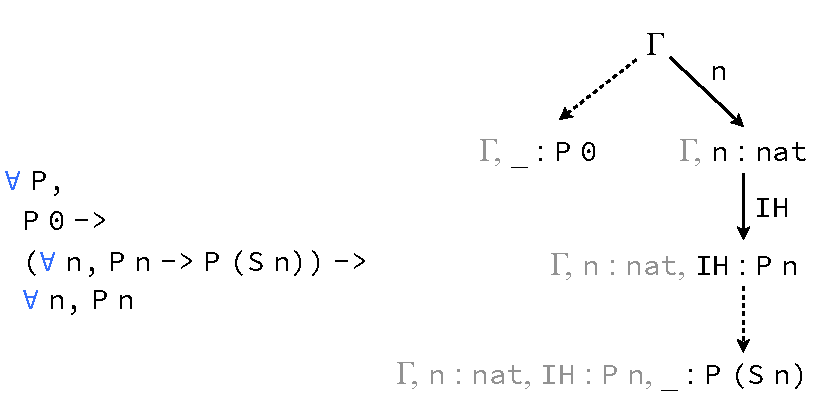
\includegraphics[scale=0.55]{repair/nat_ind}
\end{center}
\caption{The type of (left) and tree for (right) the induction principle \lstinline{nat_ind}. The solid edges represent hypotheses, and the dotted edges represent the proof obligations for each case in an inductive proof.}
\label{fig:cattree}
\end{figure}

\subsubsection{Transformations}

\paragraph{Patch Specialization} Specialization (\lstinline{specialize.ml}) takes a patch candidate and some arguments,
all of which are Coq terms.
It applies the candidate to the arguments, then it $\beta\iota$-reduces~\cite{equality} the result using Coq's
\lstinline{Reduction.nf_betaiota} function. It is the job of the 
patch finding procedure to provide both the candidate and the arguments.

\paragraph{Patch Abstraction} Abstraction (\lstinline{abstraction.ml}) takes a patch candidate, 
the goal type, and the function arguments or function to abstract.
It first generalizes the candidate, wrapping it inside of a lambda from the type of the term to abstract.
Then, it substitutes terms inside the body with the abstract term.
It continues to do this until there is nothing left to abstract, then filters results by the goal type.
Consider, for example, abstracting this candidate by \lstinline{m}:

\begin{lstlisting}[language=coq]
  fun (H : n <= m) => le_plus_trans n m 1 H(@\vspace{-0.04cm}@)
  : n <= m -> n <= m + 1
\end{lstlisting}
The generalization step wraps this in a lambda from some \lstinline{nat}, the type of \lstinline{m}:

\begin{lstlisting}[language=coq]
  fun ((@\diff{n0}@) : nat) =>(@\vspace{-0.04cm}@)
    (fun (H : n <= m) => le_plus_trans n m 1 H)(@\vspace{-0.04cm}@)
  : (@\ltacforall@) (@\diff{n0}@), n <= m -> n <= m + 1
\end{lstlisting}
The substitution step replaces \lstinline{m} with \lstinline{n0}:

\begin{lstlisting}[language=coq]
  fun ((@\diff{n0}@) : nat) =>(@\vspace{-0.04cm}@)
    (fun (H : n <= (@\diff{n0}@)) => le_plus_trans n (@\diff{n0}@) 1 H)(@\vspace{-0.04cm}@)
  : (@\ltacforall@) (@\diff{n0}@), n <= (@\diff{n0}@) -> n <= (@\diff{n0}@) + 1
\end{lstlisting}

Abstraction uses a list of \textit{abstraction strategies} to determine what subterms
to substitute. In this case, the simplest strategy works: The tool
replaces all terms that are convertible to the concrete argument \lstinline{m} with the abstract argument
\lstinline{n0}, which produces a single candidate. Type-checking this candidate confirms that it is a patch.

In some cases, the simplest strategy is not sufficient, even when it is possible to abstract the term.
It may be possible to produce a patch only by abstracting \emph{some} of the subterms
convertible to the argument or function (we show an example of this in Section~\ref{sec:fail}),
or the term may not contain any subterms convertible to the argument or function at all.
We implement several strategies to account for this. The combinations strategy, for example,
tries all combinations of substituting only some of the convertible subterms with the abstract argument. 
The pattern-based strategy substitutes subterms that match a certain pattern
with a term that corresponds to that pattern.

It is the job of the patch finding procedure to provide the candidate and the terms to abstract.
In addition, each configuration includes a list of strategies.
The configuration for changes in conclusions, for example, starts with the simplest strategy,
and moves on to more complex strategies only if that strategy fails.
This design makes abstraction simple to extend with new strategies and simple to call with different strategies
for different classes of changes.

\paragraph{Patch Inversion} Patch inversion (\lstinline{inverting.ml}) exploits symmetry to try to reverse the conclusions of a 
candidate patch.
It first factors the candidate using the factoring component, then calls the primitive inversion
function on each factor, then finally folds the resulting list in reverse.
The primitive inversion function exploits symmetry. 
For example, equality is symmetric, so the component can invert any application of \lstinline{eq_ind} or \lstinline{eq_ind_r}
(any rewrite). Indeed, \lstinline{eq_ind} and \lstinline{eq_ind_r} are inverses, and are related by symmetry:

\begin{lstlisting}[language=coq]
  (@\diff{eq\_ind\_r}@) A x P (H : P x) y (H0 : y = x) :=(@\vspace{-0.04cm}@)
    (@\diff{eq\_ind}@) x (fun y0 : A => P y0) H y ((@\diff{eq\_sym}@) H0)	
\end{lstlisting}
If inversion does not recognize that the type is symmetric, it
swaps subterms and type-checks the result to see if it is an inverse.

\paragraph{Lemma Factoring} The lemma factoring component (\lstinline{factoring.ml}) searches within a term
for its factors. For example,
if the term composes two functions, it returns both factors:

\begin{lstlisting}[language=coq]
  t : (@\diff{X}@) -> (@\diff{Z}@)                (* term *)(@\vspace{-0.04cm}@)
 [f : (@\diff{X}@) -> (@\diff{Y}@); g : (@\diff{Y}@) -> (@\diff{Z}@)] (* factors *)
\end{lstlisting}
In this case, the component takes the composite term and \lstinline{X} as arguments.
It first searches as deep as possible for a term of type \lstinline{X -> Y} for some \lstinline{Y}.
If it finds such a term, then it recursively searches for a term with type \lstinline{Y -> Z}. 
It maintains all possible 
paths of factors along the way, and it discards any paths that cannot reach \lstinline{Z}.

The current implementation can handle paths
with more than two factors, but it fails when \lstinline{Y} depends on \lstinline{X}.
Other components may benefit from dependent factoring; we leave this to future work.

\subsubsection{Inside the Procedure}
\label{sec:algimpl}

The implementation (\lstinline{patcher.ml4}) of the procedure from Section~\ref{sec:composeintro} starts with a
preprocessing step which compiles the proof terms to trees (like the tree in Figure~\ref{fig:cattree}).
It then searches for candidates one step at a time, expanding the trees when necessary.

The \sysname prototype exposes the patch finding procedure to users through the Coq 
command \lstinline{Patch Proof}. \sysname automatically
infers which configuration to use for the procedure from the example change. For example, to
find a patch for the case study in Section~\ref{sec:compcert}, we
used this command:

\begin{lstlisting}[language=ml4]
  Patch Proof Old.unsigned_range unsigned_range as patch.
\end{lstlisting}
\sysname analyzed both versions of \lstinline{unsigned_range} and determined 
that a constructor of the \lstinline{int} type changed (Figure~\ref{fig:int}),
so it initialized the configuration for changes in constructors.

Internally, \sysname represents configurations as sets of options,
which it passes to the procedure. The procedure uses these options to determine
how to compose components (for example, whether to abstract candidates) 
and how to customize components (for example, whether semantic differencing should look for an intermediate lemma).
To implement new configurations for different classes of changes, we simply tweak the options.

\subsection{Workflow Integration}

Needed: hints and so on, any work done since, the Git interface, whatever.

\subsubsection{Trusted Computing Base}
\label{sec:tcb}

A common concern for Coq plugins is an increase in the trusted computing base.
The Coq developers provide a safe plugin API in Coq 8.7 to address this~\cite{coq87news}.
Our prototype takes this into consideration:
While \sysname does not yet support Coq 8.7, it only calls the internal Coq functions that the 
developers plan to expose in the safe API~\cite{coqPR}.
Furthermore, Coq type-checks terms that plugins produce.
Since \sysname does not modify the type checker, it cannot produce an ill-typed term.


\section{Results}
\label{sec:pumpkin-results}

% TODO? Needed: key technical results (in intro though)

% below: case studies

To show how \sysname could \kl{save work for proof engineers on real proof developments}, I used the \sysname prototype to emulate three motivating scenarios from real-world code:

\begin{enumerate}
\item \textbf{Updating definitions} within a project \\
(CompCert, Section~\ref{sec:compcert})
\item \textbf{Porting definitions} between libraries \\
(Software Foundations, Section~\ref{sec:foundations})
\item \textbf{Updating proof assistant versions} \\
(Coq Standard Library, Section~\ref{sec:coq})
\end{enumerate}
The code I chose for these scenarios demonstrated different classes of changes.
For each case, I describe how \sysname configures the procedure to use differencing and transformations for that class of changes.
My experiences with these scenarios suggest that patches are useful and that both differencing and the transformations 
are effective and flexible.

\paragraph{Identifying Changes} I identified Git commits from popular Coq projects that
demonstrated each scenario.
These commits updated proofs in response to breaking changes.
I emulated each scenario as follows:

\begin{enumerate}
\item \textit{Replay} an example proof update for \sysname.
\item \textit{Search} the example for a patch using \sysname.
\item \textit{Apply} the patch to fix a different broken proof.
\end{enumerate}
My goal was to simulate incremental use of a repair tool,
at the level of a small change or a commit that follows best practices.
I favored commits with changes that I could isolate.
When isolating examples for \sysname, I replayed changes from the bottom up,
as if I was making the changes myself.
This means that I did not always make the same change as the user. For example,
the real change from Section~\ref{sec:compcert} updated multiple definitions;
I updated only one.

\sysname does not yet handle structural changes like adding constructors or parameters, 
so I focused on changes that preserve structure, like modifying constructors.
Chapter~\ref{chapt:pi} describes an extension to \sysnamelong that supports changes in structure.

\begin{figure*}
\begin{minipage}{0.49\textwidth}
\lstset{language=coq, aboveskip=0pt,belowskip=0pt}
\lstinputlisting[firstline=1, lastline=3]{repair/compcert.tex}
\lstinputlisting[backgroundcolor=\color{orange!35},firstline=4,lastline=4]{repair/compcert.tex}
\lstinputlisting[firstline=5, lastline=5]{repair/compcert.tex}
\end{minipage}
\hfill
\begin{minipage}{0.49\textwidth}
\lstset{language=coq, aboveskip=0pt,belowskip=0pt}
\lstinputlisting[firstline=7, lastline=9]{repair/compcert.tex}
\lstinputlisting[backgroundcolor=\color{orange!35},firstline=10,lastline=10]{repair/compcert.tex}
\lstinputlisting[firstline=11, lastline=11]{repair/compcert.tex}
\end{minipage}
\caption[Caption for LOF]{Old (left) and new (right) definitions of \lstinline{int} in CompCert.}
\label{fig:int}
\end{figure*}

\begin{figure*}
\begin{minipage}{0.49\textwidth}
\lstset{language=coq, aboveskip=0pt,belowskip=0pt} % blindFS / User A
\lstinputlisting[firstline=2, lastline=5]{repair/bintonat.tex}
\lstinputlisting[backgroundcolor=\color{orange!35},firstline=6,lastline=6]{repair/bintonat.tex}
\lstinputlisting[firstline=7, lastline=7]{repair/bintonat.tex}
\lstinputlisting[backgroundcolor=\color{orange!35},firstline=8,lastline=8]{repair/bintonat.tex}
\lstinputlisting[firstline=9, lastline=9]{repair/bintonat.tex}
\end{minipage}
\hfill
\begin{minipage}{0.49\textwidth}
\lstset{language=coq, aboveskip=0pt,belowskip=0pt}  % marshall / user B
\lstinputlisting[firstline=12, lastline=15]{repair/bintonat.tex}
\lstinputlisting[backgroundcolor=\color{orange!35},firstline=16,lastline=17]{repair/bintonat.tex}
\lstinputlisting[firstline=18, lastline=18]{repair/bintonat.tex}
\lstinputlisting[backgroundcolor=\color{orange!35},firstline=19,lastline=20]{repair/bintonat.tex}
\lstinputlisting[firstline=21, lastline=21]{repair/bintonat.tex}
\end{minipage}
\caption[Caption for LOF]{Definitions of \lstinline{bin_to_nat} for Users A (left) and B (right). Note that \lstinline{bin_to_nat} uses pattern matching and fixpoints
rather than \kl{primitive eliminators}, unlike most of the terms in this thesis.}
\label{fig:bintonat}
\end{figure*}

\lstset{language=coq, aboveskip=3pt,belowskip=3pt}

\subsection{Updating Definitions}
\label{sec:compcert}

Coq programmers sometimes make changes to definitions that break proofs
within the same project. To emulate this use case, 
I identified a CompCert commit~\cite{compcertcommit}
with a breaking change to \lstinline{int} (Figure~\ref{fig:int}). %The commit message notes that the new representation is more efficient.
I used \sysname to find a patch that corresponds to the change in \lstinline{int}.
The patch \sysname found fixed broken inductive proofs.

\paragraph{Replay} I used the proof of \lstinline{unsigned_range} as the example for \sysname.
The proof failed with the new \lstinline{int}:

\lstset{language=coq, aboveskip=3pt,belowskip=3pt}
\begin{lstlisting}[language=coq]
  Theorem unsigned_range:
    (@\ltacforall@)(i : int), 0 <= unsigned i < modulus.
  Proof.
    intros i. induction i using int_ind; auto(@\fails{.}@)
\end{lstlisting}
I replayed the change to \lstinline{unsigned_range}:

\begin{lstlisting}[language=coq]
    intros i. induction i using int_ind. (@\diff{simpl. omega}@)(@\succeeds{.}@)
\end{lstlisting}

\paragraph{Search} I used \sysname to search the example for a patch that corresponds to the change in \lstinline{int}. It found
a patch with this type:

\begin{lstlisting}[language=coq]
   (@\ltacforall@) z : Z, (@\diff{-1 < z < modulus}@) $\rightarrow$ (@\diff{0 <= z < modulus}@)
\end{lstlisting}

\paragraph{Apply} After changing the definition of \lstinline{int}, the proof of the
theorem \lstinline{repr_unsigned} failed on the last tactic:

\begin{lstlisting}[language=coq]
  Theorem repr_unsigned:
    (@\ltacforall@)(i : int), repr (unsigned i) = i.
  Proof.
    $\ldots$ apply Zmod_small; auto(@\fails{.}@)
\end{lstlisting}
Manually trying \lstinline{omega}---the tactic which helped us in the proof of \lstinline{unsigned_range}---did not
succeed.
I added the patch that \sysname found to a hint database.
The proof of the theorem \lstinline{repr_unsigned} then went through:

\begin{lstlisting}[language=coq]
  $\ldots$ apply Zmod_small; auto(@\succeeds{.}@)
\end{lstlisting}

\subsubsection{Instance}

This scenario used the search procedure instance for changes in constructors of an inductive type.
Given such a change:

\begin{lstlisting}[language=coq]
  Inductive (@\diff{T}@) := $\ldots$ | C : $\ldots$ $\rightarrow$ (@\diff{H}@) $\rightarrow$ T
  Inductive (@\diff{T'}@) := $\ldots$ | C : $\ldots$ $\rightarrow$ (@\diff{H'}@) $\rightarrow$ T'
\end{lstlisting}
\sysname searches in the difference between two inductive proofs of theorems:

\begin{lstlisting}[language=coq]
  (@\ltacforall@) (t : (@\diff{T}@)), P t
  (@\ltacforall@) (t : (@\diff{T'}@)), P t
\end{lstlisting}
for an isomorphism\footnote{If \sysname finds just one implication, it returns that.} between the constructors:

\begin{lstlisting}[language=coq]
  $\ldots$ $\rightarrow$ (@\diff{H}@) $\rightarrow$ (@\diff{H'}@)(@\vspace{-0.1cm}@)
  $\ldots$ $\rightarrow$ (@\diff{H'}@) $\rightarrow$ (@\diff{H}@)
\end{lstlisting}
The proof engineer can apply these patches within the inductive case that corresponds to the constructor \lstinline{C}
to fix other broken proofs that induct over the changed type. 
\sysname uses this search procedure instance for changes in constructors:

\begin{algorithm}
\footnotesize
\begin{algorithmic}[1]
    \STATE \textit{diff} inductive constructors for goals
    \STATE \textit{diff} and \textit{transform} to recursively search for changes in conclusions of the corresponding case of the proof
    \STATE \textbf{if} there are candidates \textbf{then}
    \STATE \hspace*{1em} try to \textit{invert} the patch to find an isomorphism 
\end{algorithmic}
\end{algorithm}

\subsection{Porting Definitions}
\label{sec:foundations}

Proof engineers sometimes port theorems and proofs to use definitions from different libraries.
To simulate this, I used \sysname to port two solutions~\cite{usera, userb}
to an exercise in Software Foundations to each use the other solution's definition of the fixpoint \lstinline{bin_to_nat} (Figure~\ref{fig:bintonat}).
I demonstrate one direction; the opposite was similar.

\paragraph{Replay} I used the proof of \lstinline{bin_to_nat_pres_incr} from User A as the example for \sysname.
User A cut an inline lemma in an inductive case and proved it using a rewrite:

\begin{lstlisting}[language=coq]
  assert ((@\ltacforall@)a, S (a + S (@\diff{(a + 0)}@)) = S (S (a + (@\diff{(a + 0)}@)))).
  (@\ltacba@) $\ldots$ (@\diff{rewrite $\leftarrow$ plus\_n\_O.}@) rewrite $\rightarrow$ plus_comm.
\end{lstlisting} % blindFS / user A
When I ported User A's solution to use User B's definition of \lstinline{bin_to_nat}, 
the application of this inline lemma failed. I changed the conclusion of the inline lemma 
and removed the corresponding rewrite:

\begin{lstlisting}[language=coq]
  assert ((@\ltacforall@)a, S (a + S a) = S (S (a + a))).
  (@\ltacba@) $\ldots$ rewrite $\rightarrow$ plus_comm.
\end{lstlisting} % blindFS / user A, adapted

\paragraph{Search} I used \sysname to search in the difference between the old and new versions of the example
patched proof for a patch that corresponds to the change in \lstinline{bin_to_nat}.
It found an isomorphism:

\begin{lstlisting}[language=coq]
  (@\ltacforall@)P b, P (@\diff{(bin\_to\_nat b)}@) $\rightarrow$ P (@\diff{(bin\_to\_nat b + 0)}@)(@\vspace{-0.08cm}@)
  (@\ltacforall@)P b, P (@\diff{(bin\_to\_nat b + 0)}@) $\rightarrow$ P (@\diff{(bin\_to\_nat b)}@)
\end{lstlisting}

\paragraph{Apply} After porting to User B's definition, a rewrite in the proof of the theorem
\lstinline{normalize_correctness} failed:

\begin{lstlisting}[language=coq]
  Theorem normalize_correctness:
    (@\ltacforall@)b, nat_to_bin (bin_to_nat b) = normalize b.
  Proof.
    $\ldots$ (@\fails{rewrite $\rightarrow$ plus\_0\_r.}@)
\end{lstlisting}
Attempting the obvious patch from the difference in tactics---rewriting by \lstinline{plus_n_O}---failed.
Applying the patch that \sysname found fixed the broken proof:

\begin{lstlisting}[language=coq]
   $\ldots$ (@\diff{apply patch\_inv.}@) (@\succeeds{rewrite $\rightarrow$ plus\_0\_r.}@)
\end{lstlisting}

In this case, since I ported User A's definition to a simpler 
definition,\footnote{User A uses \lstinline{*}; User B uses \lstinline{+}. 
For arbitrary \lstinline{n}, the term \lstinline{2 * n} reduces to \lstinline{n + (n + 0)}, which does not reduce any further.}
\sysname found a patch that was not the most natural patch.
The natural patch would be to remove the rewrite, just as I removed a different rewrite from the example proof.
This did not occur when I ported User B's definition,
which suggests that in the future, a patch finding tool may help inform novice users which definition is simpler:
It can factor the proof,  
then inform the user if two factors are inverses.
Tactic-level changes do not provide enough information to determine this; the tool must have a semantic
understanding of the terms.
My Magic tutorial plugin~\footnote{\url{https://github.com/uwplse/magic}} % TODO static link
implements a prototype of the functionality needed for this, based on lessons from this case study.

\subsubsection{Instance}

This scenario used the search procedure instance for changes in cases of a fixpoint.
Given such a change:

\begin{lstlisting}[language=coq]
  Fixpoint (@\diff{f}@) $\ldots$ := $\ldots$ | g (@\diff{x}@)(@\vspace{-0.1cm}@)
  Fixpoint (@\diff{f'}@) $\ldots$ := $\ldots$ | g (@\diff{x'}@)
\end{lstlisting}
\sysname searches in the difference between two versions of proofs of the theorems:

\begin{lstlisting}[language=coq]
  (@\ltacforall@) $\ldots$, P ((@\diff{f}@) $\ldots$)(@\vspace{-0.1cm}@)
  (@\ltacforall@) $\ldots$, P ((@\diff{f'}@) $\ldots$)
\end{lstlisting}
for an isomorphism that corresponds to the change:

\begin{lstlisting}[language=coq]
  (@\ltacforall@)P, P (@\diff{x}@) $\rightarrow$ P (@\diff{x'}@)(@\vspace{-0.1cm}@)
  (@\ltacforall@)P, P (@\diff{x'}@) $\rightarrow$ P (@\diff{x}@)
\end{lstlisting}
The proof engineer can apply these patches to fix other broken proofs about the fixpoint.

The key feature that differentiates these from the patches we have encountered so far is that
these patches hold for \emph{all} \lstinline{P}; for changes in fixpoint cases, the procedure generalizes
candidates by \lstinline{P}, not by its arguments.
\sysname uses this search procedure instance for changes in fixpoint cases:

\begin{algorithm}
\footnotesize
\begin{algorithmic}[1]
    \STATE \textit{diff} fixpoint cases for goals
    \STATE \textit{diff} and \textit{transform} to recursively search within an intermediate lemma for a change in conclusions
    \STATE \textbf{if} there are candidates \textbf{then}
    \STATE \hspace*{1em} \textit{specialize} and \textit{factor} the candidate \\
           \hspace*{1em} \textit{generalize} the factors by functions \\
           \hspace*{1em} try to \textit{invert} the patch to find an isomorphism 
\end{algorithmic}
\end{algorithm}

For the prototype, I require the user to cut the intermediate lemma explicitly and to 
pass its type and arguments.
In the future, an improved semantic differencing component
can infer both the intermediate lemma and the arguments: it can search
within the proof for some proof of a function that is applied
to the fixpoint.

\begin{figure*}
\begin{minipage}{0.48\textwidth}
\lstset{language=coq, aboveskip=0pt,belowskip=0pt}
\lstinputlisting[firstline=1, lastline=1]{repair/divide.tex}
\end{minipage}
\hfill
\begin{minipage}{0.48\textwidth}
\lstset{language=coq, aboveskip=0pt,belowskip=0pt}
\lstinputlisting[firstline=3, lastline=3]{repair/divide.tex}
\end{minipage}
\caption[Caption for LOF]{Old (left) and new (right) definitions of \lstinline{divide} in Coq.}
\label{fig:divide}
\end{figure*}

\lstset{language=coq, aboveskip=3pt,belowskip=3pt}

\subsection{Updating Proof Assistant Versions}
\label{sec:coq}

Coq sometimes makes changes to its standard library that break
backwards compatibility.
To test the plausibility of using a patch finding tool for proof assistant version updates,
I identified a breaking change in the Coq standard library~\cite{coq84commit}.
The commit changed the definition of \lstinline{divide} prior to the Coq 8.4 release (Figure~\ref{fig:divide}).
The change broke 46 proofs in the standard library.
I used \sysname to find an isomorphism that corresponds to the change in \lstinline{divide}.
The isomorphism \sysname found fixed broken proofs.

\paragraph{Replay} I used the proof of \lstinline{mod_divide} as the example for \sysname.
The proof broke with the new \lstinline{divide}:

\begin{lstlisting}[language=coq]
  Theorem mod_divide:
    (@\ltacforall@) a b, b~=0 $\rightarrow$ (a mod b == 0 $\leftrightarrow$ (divide b a)).
  Proof.
    $\ldots$ (@\fails{rewrite (div\_mod a b Hb) at 2.}@)
\end{lstlisting}
I replayed changes to \lstinline{mod_divide}:

\begin{lstlisting}[language=coq]
    $\ldots$ (@\diff{rewrite mul\_comm. symmetry.}@)
    (@\succeeds{rewrite (div\_mod a b Hb) at 2.}@)
\end{lstlisting}

\paragraph{Search} I used \sysname to search within the example patched proof for a patch
that corresponds to the change in \lstinline{divide}.
It found an isomorphism:

\begin{lstlisting}[language=coq]
   (@\ltacforall@)r p q, (@\diff{p * r = q}@) $\rightarrow$ (@\diff{q = r * p}@)(@\vspace{-0.08cm}@)
   (@\ltacforall@)r p q, (@\diff{q = r * p}@) $\rightarrow$ (@\diff{p * r = q}@)
\end{lstlisting}

\paragraph{Apply} The proof of the theorem \lstinline{Zmod_divides} broke after rewriting by the changed theorem \lstinline{mod_divide}:

\begin{lstlisting}[language=coq]
  Theorem Zmod_divides:
    (@\ltacforall@)a b, b<>0 $\rightarrow$ (a mod b = 0 $\leftrightarrow$ (@\ltacexists@)c, a = b * c).
  Proof.
    $\ldots$ split; intros (c,Hc); exists c; (@\fails{auto.}@)
\end{lstlisting}
Adding the patches \sysname found to a hint database made the proof go through:

\begin{lstlisting}[language=coq]
    $\ldots$ split; intros (c,Hc); exists c; (@\succeeds{auto.}@)
\end{lstlisting}

\subsubsection{Instance}

This scenario used the search procedure instance for changes in dependent arguments to constructors.
\sysname searches within the difference between two versions of a proof that apply the same constructor
to different dependent arguments:

\begin{lstlisting}[language=coq]
   $\ldots$ (C ((@\diff{P}@) x)) $\ldots$(@\vspace{-0.1cm}@)
   $\ldots$ (C ((@\diff{P'}@) x)) $\ldots$
\end{lstlisting}
for an isomorphism between the arguments:

\begin{lstlisting}[language=coq]
   (@\ltacforall@) x, (@\diff{P}@) x -> (@\diff{P'}@) x(@\vspace{-0.1cm}@)
   (@\ltacforall@) x, (@\diff{P'}@) x -> (@\diff{P}@) x
\end{lstlisting}
The proof engineer can apply these patches to patch proofs that apply the constructor (in this case study,
to fix broken proofs that instantiate \lstinline{divide} with some specific \lstinline{r}).

So far, we have encountered changes of this form as arguments to an 
induction principle; in this case, the change is an argument to a constructor.
A patch between arguments to an induction principle maps
directly between conclusions of the new and old theorem without
induction; a patch between constructors does not.
For example, for \lstinline{divide}, we can find a patch with this form:

\begin{lstlisting}[language=coq]
   (@\ltacforall@)x, (@\diff{P}@) x $\rightarrow$ (@\diff{P'}@) x
\end{lstlisting}
However, without using the induction principle for \lstinline{exists}, we can't use that patch to prove this:

\begin{lstlisting}[language=coq]
   ((@\ltacexists@)x, (@\diff{P}@) x) $\rightarrow$ ((@\ltacexists@) x, (@\diff{P'}@) x)
\end{lstlisting}
This changes the goal type that semantic differencing determines.

\sysname uses this search procedure instance for changes in constructor arguments:

\begin{algorithm}
\footnotesize
\begin{algorithmic}[1]
    \STATE \textit{diff} constructor arguments for goals
    \STATE \textit{diff} and \textit{transform} to recursively search within those arguments for changes in conclusions
    \STATE \textbf{if} there are candidates \textbf{then}
    \STATE \hspace*{1em} \textit{generalize} the candidate \\
           \hspace*{1em} \textit{factor} and try to \textit{invert} the patch to find an isomorphism
\end{algorithmic}
\end{algorithm}
For the prototype, the model of constructors for the semantic differencing component is limited,
so \sysname asks the user to provide the type of the change in argument (to guide line 2).
Extending semantic differencing may help remove this restriction.






\chapter{Conclusions \& Future Work}
\label{chapt:conclusions}

Through a combination of differencing and proof term transformations,
my proof repair tool suite can extract, generalize, and apply the information that a change carries to fix proofs broken by the same change.
Proof repair can save and in fact already has saved work for proof engineers relative to reference manual repairs in practical use cases.
And so proof repair is reason to believe that verifying a modified system should often, in practical use cases, be easier than verifying the original the first time around,
even when proof engineers do not follow good development processes,
or when change occurs outside of proof engineers' control.

Do not just take my word for it.
Consider a recent article by a proof engineer saying just this (emphasis mine): % TODO link: https://galois.com/blog/2020/12/proofs-should-repair-themselves/

\begin{quote}
We have \textit{reason to think} such proof repair is tractable. Rather than trying to synthesize a complete proof from nothing---a problem known to be immensely difficult---we 
start from a correct proof of fairly similar software. We will be attempting proof reconstruction \textit{within a known neighborhood}.
\end{quote}
The proof engineer credited my proof repair work on Twitter, % TODO link to Twitter
but noted that there ought to be much more work in this space.

I agree.
Actually, I want to take that a step further:
proof repair is just a small piece of what will carry us to the next era of proof engineering.
And that era will be one in which programmers of all skill levels across all domains can develop and maintain verified systems---the era of
\textit{proof engineering for all}.

\section*{The Next Era: Proof Engineering for All}

% 2030? could do decades for each of this lol. I guess only if energy
% Do just 2-3 sentences per project.

Proof engineering has come a long way, but it is still accessible mostly to experts, and perhaps the occasional practitioner.
Proof repair has made proof engineering easier for experts, and a bit easier for practitioners.
But there is a lot more that we as a community can do to bring proof engineering to all: not just experts and practitioners,
but also software engineers and potential users from in other domains.

I conclude with a discussion of 12 future project ideas building up to the next era of proof engineering for all.
If any of these ideas inspire you, please work with me to bring them to life.

\subsection*{Experts}

In the future, maintaining proofs ought to be seamless for expert proof engineers.
Ideally, this means technologies---like proof repair---that automate everything but the creative parts of maintenance tasks,
leaving the creativity to the experts.
But the maintenance technologies of the future ought to reach all proof assistants,
be much more powerful,
and produce natural proof scripts in the end.

\paragraph{All Proof Assistants}
Proof repair ought to be accessible across all proof assistants.
The techniques from this thesis should be simple to apply to proof assistants with similar foundations to Coq, like Agda,
and potentially Lean.\footnote{Lean assumes an axiom that is incompatible with univalence.
It is not quite clear to me what that assumption would mean for implementing the \toolnamec transformation in Lean.
Everything else should carry over.}
But Isabelle/HOL, for example, lacks proof terms and is based on a classical logic.
One path toward proof repair for Isabelle/HOL may be to reify proof terms using
Isabelle/HOL-Proofs, apply a transformation based on the Transfer~\cite{Huffman2013} package for proof reuse, and then (as in \toolnamec) decompile those terms to automation that does 
not apply Transfer or refer to the old datatype.
Similar approaches may work for other proof assistants.

\paragraph{More Power} 
Proof repair ought to be much more powerful than it is right now.
%For example, the repair tools of the present have only limited support for proof assistant version updates;
%the repair tools of the future ought to run automatically in response to version updates, and ought to support fundamental changes in the proof term
%or proof script language.
The repair tools of the future ought to run automatically in response to proof assistant version updates.
%, and ought to support
%fundamental changes in the proof term or proof script language.
They ought to break down large changes into smaller pieces---perhaps by drawing on work in change and 
dependency management~\cite{873647, Autexier:2010:CMH:1986659.1986663, Celik:2017:IRP:3155562.3155588} to identify changes, then use the factoring transformation
to break those changes into smaller parts.
And they ought to support an even broader and more practical class of changes than they do now,
like arbitrary relations.

\paragraph{Natural Proofs}
Proof repair tools ought to produce repaired proof scripts that are natural for expert proof engineers,
regardless of style.
Toward this end, I have just begun a promising project with \kl{RanDair} and some collaborators at UMass Amherst
on integrating the prototype decompiler with the machine learning proof synthesis tool TacTok~\cite{10.1145/3428299} to rank tactic hints.
Producing more natural proofs than the prototype decompiler using fixed training data seems feasible.
More difficult---but desirable---is to train the decompiler to produce scripts that match the style of the proof engineer using the tool.

\subsection*{Practitioners}

In the future, developing and maintaining proofs ought to be much easier for practitioners to use.
Proof engineering is just starting to reach practitioners, and my proof repair tools have been a small part of that.
Workflow integration has been central to that effort, but there is a long way to go.
The repair tools of the future ought to include much more automation,
integrate smoothly into IDEs and CI tools,
and continually improve in response to feeedback from user studies.

\paragraph{More Automation}
Proof repair tools ought to include much more automation.
They ought to elegantly support repair over large libraries when many changes occur at once,
while imposing little additional effort on the proof engineer.
They ought to be simple to extend with new optimizations, all while preserving correctness.
One promising path to these ends is integrating the \toolnamec transformation with \textit{e-graphs}~\cite{egraph1},
a data structure %that is used in the constraint solver and rewrite system communities 
for managing equivalences
built with these kinds of problems in mind.
E-graphs were recently adapted to express path equality in cubical~\cite{egraph6}---a perfect fit for the \toolnamec transformation.
E-graphs in other proof assistants, like those in Lean~\cite{selsam:lean}, could help with similar automation for repair tools for other proof assistants.

\paragraph{Smooth Integration}
Proof repair tools ought to integrate smoothly into IDEs like Proof General~\cite{proofgeneral},
or into continuous integration (CI) systems like Travis~\cite{travis}.
CI support hinges on the ability to break large changes into smaller pieces.
At the level of the IDE, recording changes during development may help circumvent this problem.
The infrastructure from the \textsc{REPLica} user study may be a good start for IDE integration.
Program repair tools like CatchUp!~\cite{Henkel:2005:CCR:1062455.1062512} with existing IDE integration may provide inspiration
for both infrastructure and user experience.

\paragraph{User Feedback} 
Proof repair tools ought to continually adapt to feedback from the proof engineers who use them.
This means user studies not just of proof engineers using proof assistants (like the \textsc{REPLica} user study),
but also of proof engineers using proof repair tools.
The same principle applies to other proof engineering tools.
The \textsc{REPLica} user study paper discusses many important challenges of and potential solutions to conducting user studies
of proof engineers, and can serve as inspiration for the design.

\subsection*{Software Engineers}

In the future, proof engineering ought to be accessible to software engineers.
Even with good proof engineering technologies, it is not always economically feasible or even desirable for software engineers to formally verify 
an entire system using a proof assistant.
This makes a strong case for \textit{mixed methods verification}:
verification using multiple techniques while guaranteeing that their composition preserves correctness.
I advocated for this in the survey paper~\cite{PGL-045}, and I implemented one case of this at Galois: using
\sysnamelong to help a proof engineer interoperate between a constraint solver and Coq.
The repair tools of the future ought to similarly integrate with tools familiar to software engineers,
help software engineers infer specifications,
and assist software engineers in redesiging code for verification.

\paragraph{Familiar Tools} A continuum from testing to verification, tools to help with that.

\paragraph{Specification Inference} Analysis to infer specs (TA1).

\paragraph{Tool-Assisted Redesign} Tool-assisted development to follow good design principles for verificattion (James Wilcox conversation, final REPLICA takeaway).

\subsection*{New Domains}

Unifying theme: collaboration, new abstractions for new domains). Some examples:

\paragraph{Machine Learning} Fairification \& other ML correctness properties. Some stuff here but more.

\paragraph{Cryptography} Lots of stuff here but not thinking broadly enough. What about cryptographic proof systems? ZK and beyond. Recall email thread.

\paragraph{Something Else} Look for more in survey paper, email, DARPA TAs, Twitter. Healthcare perhaps? % https://twitter.com/TaliaRinger/status/1373747841944883201



